\documentclass[12pt,a4paper,final,twoside,openright]{report}
\usepackage[utf8]{inputenc}
\usepackage[T1]{fontenc}
\usepackage[english]{babel}

\usepackage{hyperref}
\usepackage{url}

\usepackage{setspace}
\onehalfspacing

\usepackage{amsmath}
\usepackage{amssymb}
\usepackage{mathtools}
\usepackage{multirow}
\usepackage{graphicx}
\usepackage{caption}
\usepackage{subcaption}
\usepackage{framed}

\usepackage[ampersand]{easylist}

\usepackage{array}
\usepackage{multirow}
\usepackage{tabulary}

\usepackage{float}

\usepackage[left=2.5cm,right=2.5cm,top=2.5cm,bottom=2.5cm]{geometry}

\usepackage{appendix}

%\usepackage[nomain,acronym,toc]{glossaries}
% nomain, if you define glossaries in a file, and you use 
%\include{./Glossari/glossari}
%\makeglossaries

%Pendent el fer el glossari

\usepackage{imakeidx}
\makeindex

\usepackage{wrapfig}

%\usepackage{makeidx}
%\makeindex

\usepackage{fancyhdr}
\pagestyle{fancy}
\fancyhead{}
\fancyhead[RO,LE]{\thepage}
\fancyhead[RE,LO]{Grasping by Romeo robot using V4R}
\fancyfoot{}
\fancyfoot[RO,LE]{
\includegraphics[width=0.065\textwidth]{images/TU_small_logo.png}}

\usepackage{etoolbox}
\patchcmd{\chapter}{\thispagestyle{plain}}{\thispagestyle{fancy}}{}{}

\headheight = 15pt %Donava un warning sino

\textheight = 690pt %Col·locació de l'escut a distancia que quedi be
\footskip = 60pt

\usepackage[numbers]{natbib}
\bibliographystyle{plainnat} 
%Poso per ordre d'pració (així) o per ordre d'autors (plainnat)?

\title{Grasping by Romeo robot using V4R}
\author{Lluís Salord Quetglas\\
		\texttt{l.salord.quetglas@gmail.com}\\}
\date{Technischen Universität Wien (TU Wien)\\
Automation and Control Institute (ACIN)\\
\paragraph{} 
Master Thesis Project\\
\paragraph{}
\today} %NO FIXAR-SE AMB AIXÒ JA QUE LA PORTADA SERÀ LA DONADA PER L'ESCOLA

\usepackage{chngcntr}
\counterwithin{figure}{chapter}%Permet que el comptatge de les figures sigui segons capitol
\counterwithin{table}{chapter}
\counterwithin{equation}{chapter}
\counterwithin{footnote}{chapter}

%PLANTEJAR TEMA DE \autoref{} ja que així l'hiperenllaç es també per la paraula i no sols el numero.

\renewcommand{\thefigure}{\arabic{chapter}.\arabic{figure}}
\renewcommand{\thetable}{\arabic{chapter}.\arabic{table}}
\renewcommand{\theequation}{\arabic{chapter}.\arabic{equation}}
\renewcommand{\thefootnote}{\arabic{footnote}}

\usepackage{parskip}

\setlength{\parindent}{1em}
\usepackage{indentfirst}

\usepackage{color}

\usepackage[official]{eurosym}

\usepackage{epstopdf}

\usepackage{footnote}
\usepackage{cleveref}[2012/02/15]% v0.18.4; 
% 0.16.1 of May 2010 would be sufficient, but what is the exact day?

\crefformat{footnote}{#2\footnotemark[#1]#3}	
\usepackage{tikz}

% Make that a cell have a line break
\newcommand{\specialcell}[3][c]{%
	\begin{tabular}[#1]{@{}#2@{}}#3\end{tabular}
	}
\makeatletter
\def\z#14#2!!{\def\TY@classz{#17#2}}
\expandafter\z\TY@classz!!
\makeatother

\usepackage{listings} %To put code in the right way 
\lstset{
	basicstyle=\footnotesize,
    frame=single,
    breaklines=true,
    postbreak=\raisebox{0ex}[0ex][0ex]{\ensuremath{\color{red}\hookrightarrow\space}}
}
\lstdefinelanguage{ROS}{
    keywords = {
        rosrun, roslaunch, rostopic, rosparam
    },
    morekeywords = {command, ns, file}
}

% Used to make possible have matrix with format like [ccc|c]
\makeatletter
\renewcommand*\env@matrix[1][*\c@MaxMatrixCols c]{%
  \hskip -\arraycolsep
  \let\@ifnextchar\new@ifnextchar
  \array{#1}}
\makeatother

\begin{document}
\maketitle
\thispagestyle{empty}

\cleardoublepage

\pagenumbering{roman} % restart page numbers at one, now in roman style

\begin{abstract}
%\addcontentsline{toc}{chapter}{Abstract}

\end{abstract}

\tableofcontents
\newpage
\listoffigures
\newpage
\listoftables
\newpage

\chapter*{Acknowledgements}
\addcontentsline{toc}{chapter}{Acknowledgements}

%\chapter*{Preface}
%\addcontentsline{toc}{chapter}{Preface}

\chapter{Introduction}
\pagenumbering{arabic} % restart page numbers at one, now in arabic style

\section{Motivation}

A world with humanoids robots living with people is one of the dreams of any robotic researcher. Although, these robots should be able to do a wide range of tasks as humans or even better. However, a good interaction of robots with the surrounding environment, including humans, is so difficult to accomplish due to the complexity of it. There are several ways of interaction such as: (1) learning about the environment, (2) be able to move to wherever or (3) grasping all kind of object. All these fields are being studied in any robotic research institute but not all of them can implement it on real robots. Luckily for me, in the ACIN of the TU Wien, they have an humanoid robot, Romeo robot from Aldebaran Robotics, and I have chosen to use it focusing in the grasping process. Therefore, in this dissertation, it is made an approach of the grasping part using Romeo from Aldebaran Robotics. Moreover, before the grasp the robot should analyse the surroundings, recognise the object and then grasp it. Therefore, it should know how to recognise things, which is also a very important field.  

%\section{Definition of the project}

\section{Presentation of the problem}
%Proposit inicial de Romeo i perque necessita de fer un grasping

Romeo is an humanoid robot from Aldebaran Robotics company. Nao and Pepper are other humanoids from this company, these three belong to the Aldebaran's robot family, Figure \ref{fig:aldebaran_family}, with and specific aim for each robot. On one hand, Nao is targeted to investigation, programming and learning. On the other hand, Pepper is focused in social relations with clients or users. Finally, Romeo has the aim to help old people or people who has some kind of disability.	

\begin{wrapfigure}[10]{r}{0.4\textwidth}
	    \centering
		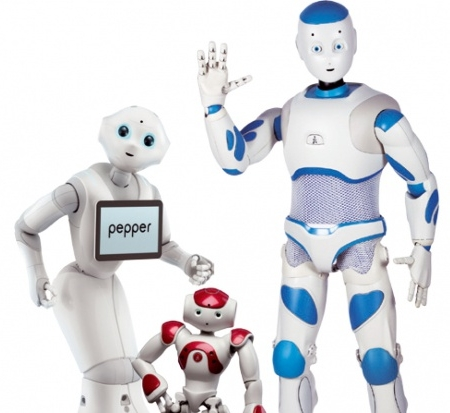
\includegraphics[width=0.35\textwidth]{images/romeo_nao_pepper.jpg}
         \caption{Aldebaran's robot family. Pepper on the left; Romeo on the right and Nao in the middle \cite{ParPaul}. \label{fig:aldebaran_family}}
\end{wrapfigure}

In order to be able to achieve this aim, Romeo has to be capable of doing several tasks, which a lot of them requires to recognize objects and grasping them. Therefore, recognition and grasp objects is a huge step forward for the development of Romeo. 

Currently, exists some approaches to grasp objects with several robots, but there is only one for Romeo  \cite{claudio:hal-01159882}, which is explained in Section \ref{sec:grasping_romeo_visual_servoing}, but it can not be used to achieve the main aim of Romeo. Therefore, it should be done a grasp approach in a way which consider this main goal.  

\section{Aim of the project}

The main goal of this project is to achieve that the Romeo robot can recognise some specific objects and, if they are inside its workspace, then grasp them. It is known that this task is difficult to accomplish, due to the wide range of parts that are involve, as recognition, movement of the robot, interaction with the environment, etc. So another goal is to discern from where it comes the main error and solve it or at least propose possible solutions. Moreover, another important goal of this project is to do the task of grasping in the way of the aim of Romeo. Therefore, it has to be coherent with the idea of helping people.

Furthermore, this task is not only important for Romeo, a wide range of robots need to achieve that. Therefore, share the code and make it open source could help other research programs, and other people could help to continue and improve our work. So this work is not over when the master thesis is done, but it can be continued with any restrictions. Moreover, the code of this project should be put in a package, which should be as flexible as possible to be complemented with any kind of packages. Finally, another main goal of this project is to be explained in a way that other people can understand perfectly how it works and then improve the code.

\section{Extent of project}

Due to the nature of the project itself there are some limitations or requirements that it should be accomplish. Firstly, it needs to be stated that this work is a first approach to make Romeo capable to recognize and grasp objects. Due to be a master thesis, which it should be done in only a few months, and it is required some time to get used with the robot, it is probably that the final result won't be totally perfect.

Furthermore, there are some software constraints which should be accomplished. On one hand, the use of an acknowledged software like ROS, explained in Section \ref{sec:ROS}, so it can be easily implemented with other packages and it is a perfect framework for a open-source robotic project. On the other hand, the use of the V4R software, explained in Section \ref{sec:V4R}, which is from our institute (ACIN), due to is a novel software for the recognition of objects. Finally, the packages from which this project depends should be used as they are officially. So if they need to be modify, the changes should be send to the maintainer of the package and updated.

\section{Repository}

One of the main ideas of this project is to be open source, so everybody can use and improve it. In order to accomplish this, all the code can be found in the following repository with also this document:

\url{https://github.com/lluissalord/romeo_grasper}

\section{Structure}

As the idea of this document is to help people, who want to use or improve the package, to understand all the parts, the document is structures as Chapter \ref{cha:pre_studies} explains some knowledge that should be known before to understand perfectly all the document. Chapter \ref{cha:design} is a brief summary of how it works the package and the most important if only wants to know how to use the package. Chapter \ref{ch:implementation} describes in detail all the parts of the package. In Chapter \ref{cha:experiments} are shown several experiments to see how precise is the package in any part. Chapter \ref{cha:discussion} explains the results from the previous chapter. Chapter \ref{cha:future_works} proposes several fields to improve the package. Finally, Chapter \ref{cha:conclusions} explains the conclusions of the project.

\chapter{Related works}
%TODO
%Posar una introduccio dels related works

%Aqui hauria de ser que trobes colcuna cosa d'altres robots que ja fan algo per l'estil.
%CERCAR ALGO A VEURE!!

\section{Grasping by Romeo with visual servoing}
\label{sec:grasping_romeo_visual_servoing}

Firstly, talk about a work previously done by another research group. The work \cite{claudio:hal-01159882} consist in grasping an object using visual servoing. The robot has to detect and to track with its gaze a box placed on a table in front of him, estimate the pose of the box with respect to one of its eye's camera, approach its arm near the box and then move the arm using visual feedback so that it is able to grasp the box accurately. Once this is achieved, it detects a human and delivers the box. A video demonstration can be found at \cite{InriaLagadicgroup}.

In order to know where is the hand with respect to the eye's camera, the hand have a QR-Code. So firstly it moves the arm in a close position to the box using odometry, then with the detection of the QR-Code compute the pose and finally using visual servoing get the arm closer to the box.

The approach proposed, grasping with visual servoing, is a good initial approach, but it is not appropriate to achieve the main Romeo's goal of helping old people or people who has some kind of disability. Firstly, it only can accomplish the grasp with one arm, and, in a complex environment, probably it should be necessary to use both arms. Secondly, to know where is the hand it needs a specific position for the head, looking at the hand, and then track it all the time. However, Romeo is supposed to have a good interaction with humans, but this features doesn't help it.

\section{MoveIt simple grasps}
\label{sec:moveit_simple_grasps}

On the ROS environment exists some packages with the aim of generate grasps, one of them and very useful to do a first approach to grasping is the \texttt{moveit\_simple\_grasps} package. This one is thought to be used with simple object as blocks or cylinders. The package generate a lot of potentials grasps taking as an input position and orientation of the object. Firstly, is needed a configuration file that describes the geometry of the robot's end effector. Currently the tested robots are Baxter and REEM, but there are some more of the mentioned configuration files for others robots such as Romeo, Pepper, Nao and Clam. For Romeo the configuration file is named \texttt{romeo\_grasp\_data.yaml}, but the most recent version of the file is in this repository \cite{gitNlyubovaGrasp}. It should be stated that this one has been designed to use the left arm to made a side grasp and the right arm for a top grasp.

Finally, the way of generate grasps for this package is trying all the directions, with a given resolution, in the plains made by the X-Z axis and by the Y-Z axis. The source of the official package with this and more information can be found at \cite{gitMoveitSimpleGrasp}.

%TODO
% Posar una imatge dels posibles grasps?

\section{AGILE grasp}
\label{sec:agile grasp}

\textit{AGILE} (\textbf{A}ntipodal \textbf{G}rasp \textbf{I}dentification and \textbf{LE}arning) grasp is a ROS package \cite{Pas} which localize antipodal grasps\footnote{In an antipodal grasp, the robot hand is able to apply opposite and co-linear forces at two points where the line connecting the contact points lies inside both friction cones \cite{DBLP:journals/corr/PasP15}.} in 3D point clouds. This work \cite{DBLP:journals/corr/PasP15} proposes a new approach to using machine learning to detect grasp poses on novel objects presented in clutter. The input to the algorithm is a point cloud and the geometric parameters of the robot hand. The output is a set of hand poses that are expected to be good grasps. According to \cite{DBLP:journals/corr/PasP15}, the grasp success rate with this algorithm is $87.8 \%$ for objects presented in isolation and $73 \%$ for objects presented in clutter. 

Firstly, it is used the geometry information to reduce the size of the sample space. In order to do that the grasps have to fulfil the condition of the hand must be collision -free and part of the object surface must be contained between the two fingers. Secondly, the geometry is also used to automatically label the training set. In order to label a subset of grasp hypotheses is used the condition of having an antipodal configuration. Therefore, a large amount of training data can be used and so improving the performance.

\section{Romeo MoveIt Config}
\label{sec:romeo_moveit_config}

At some point is necessary to use an interface and simulations to work with a robot. An option to do this, using the MoveIt platform, is the \texttt{romeo\_moveit\_config}. This package gives the necessary configuration files and launchers to use MoveIt with Romeo. Therefore, it allow to launch Rviz with a model of Romeo and interact with it. This model can represent a simulation or a real one which should be connected to ROS.

There are two main launch files: (1) \texttt{demo.launch}, which run Rviz with MoveIt and a Romeo model but executing a fake joint control, so doesn't move the real joints; (2) \texttt{moveit\_planner.launch}, the same as before but this time it moves the real joints. Inside both files it also launchs the \texttt{move\_group} class which allows to use a planner for the movements of some groups of links and joints. This class is explained with more details in the next section.

\section{Romeo MoveIt Actions}
\label{sec:romeo_moveit_actions}

%TODO
% Explicar que és el que he fet per millorar aquest package. MIRAR COMMIT GITHUB. Creació de la funció publishPlanInfo que du a terme el càlcul de la distancia entre l'últim punt de la trajectoria del pla i la posició objectiu a més de publicar la trajectoria final. També s'ha permes que de forma externa es puguin modificar els parametres de la classe un cop creada (posar parametres). També permet tenir un flag que determina si s'ha d'executar el pla o no en fer el reachAction i executeAction. Finalment correcció de petits falls del package

As the last one, the \texttt{romeo\_moveit\_action} package allow to use \texttt{moveit\_simple\_grasps} with Romeo. Moreover, it also use the \texttt{move\_group} class to make an easier use of high level commands such as reach to pose, pick or place at a pose, among others. In Figure \ref{fig:moveit_internal} can be seen the relation between these packages and their main functions. Therefore, the \texttt{romeo\_moveit\_action} package should allow the user to control Romeo to do tasks as picking or placing.

\begin{figure}[h]
\centering
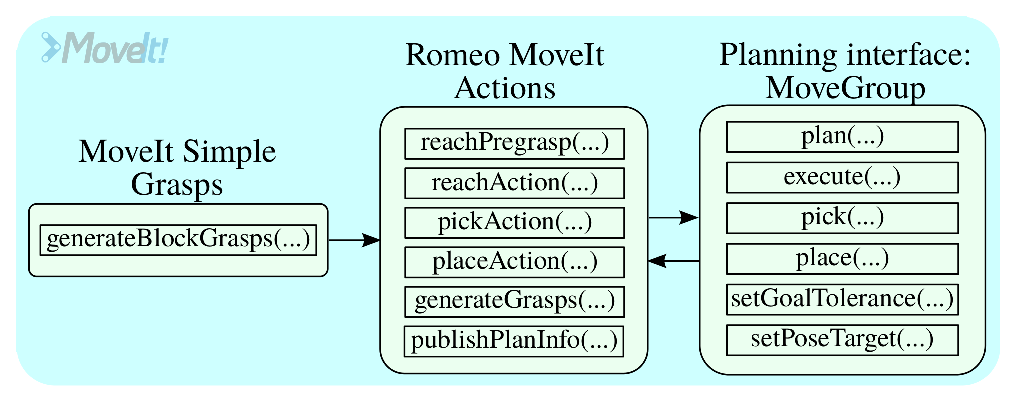
\includegraphics[width=0.8\textwidth]{images/moveit_internal.eps}
\caption{Main functions of the necessary packages for Romeo MoveIt Actions\label{fig:moveit_internal}}
\end{figure}

Firstly, before start to describe \texttt{romeo\_moveit\_action}, is necessary to explain a bit the \texttt{move\_group} class. This is the class in MoveIt that controls the current state, the target state, the planner and the movement of a group of links and joints. These groups are defined in an specific \texttt{.srdf} file in \texttt{romeo\_moveit\_config}. Usually, to work with a robot like this, with 7 DoF, is used the \texttt{left\_arm} or \texttt{right\_arm} group with \texttt{left\_hand} or \texttt{right\_hand} group as end effector, this is explained in Section \ref{sec:romeo_hardware}.

In order to be able to make plans and execute the movements, the \texttt{move\_group} class is working together with the simulator Rviz and the pertinent solver. Moreover, can be set a tolerance for the goal and the target state of the plan can be set as a: (1) pose on a reference or (2) joint state.

%TODO
% MIRAR A VEURE QUE CONVE MES FER FEINA AMB REACHACTION O GRASPPLAN!!!

Referring to \texttt{romeo\_moveit\_action} package, the most important part is the planning and execution of the grasping. Although, there are two ways of doing that: 

\begin{itemize}
\item Using \texttt{graspPlan} function, Figure \ref{fig:moveit_actions_grasp_plan}.
\item Using \texttt{reachAction} function, Figure \ref{fig:moveit_actions_reach_action}.
\end{itemize}

The main differences between one and other are: 
\begin{enumerate}
\item How to calculate the target pose 
\begin{enumerate}
\item \texttt{reachAction} use the geometry of the gripper given by \texttt{romeo\_moveit\_config} and put the target pose in a way that the gripper will be close to the object, but without touching it.
\item \texttt{graspPlan} use \texttt{moveit\_simple\_grasps} to generate all the possible grasps and choose one of them to make a plan.
\end{enumerate}

\item Attempts and approximate solutions
\begin{enumerate}
\item \texttt{reachAction} first try with different tolerances till the plan succeeded or reach the maximum attempts. In this last case, try to get an approximate solution.
\item \texttt{graspPlan} only try with one tolerance, but, as said before, it tries a lot of different grasps.
\end{enumerate}
\end{enumerate}

Once the gripper is at the right position is time to make the picking. Therefore, is used the \texttt{pickAction} function to pick the object, Figure \ref{fig:moveit_actions_pick_action}. In this case is used again the grasps generated by \texttt{moveit\_simple\_grasps}, but this time in the picking stage. This function executes automatically the movement when, after testing all the pickings, there is at least one that works.

Furthermore, there is another interesting function named \texttt{publishPlanInfo} which publish in \texttt{/trajectory} topic the planned trajectory and the last position of the plan. Moreover, it calculates the distance between target position and the final position of the plan. Although, the trajectory is in the joint space, using the forward kinematics can know the position of the final position. Finally, a summary of the topics and services used and provided by \texttt{romeo\_moveit\_actions} is showed in Figure \ref{fig:moveit_actions_ROS}. 

\begin{figure}[!h]
\centering
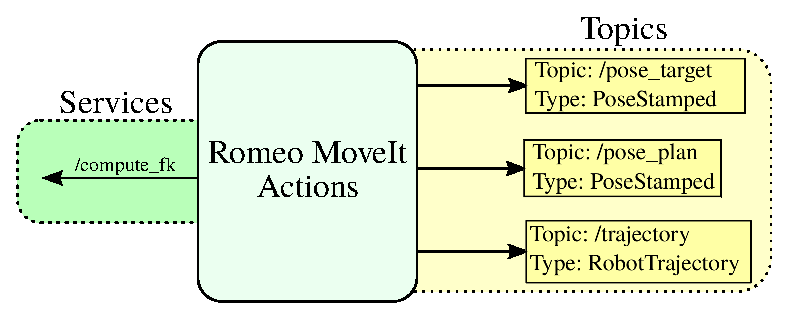
\includegraphics[width=0.8\textwidth]{images/moveit_actions_ROS.eps}
\caption{Topics and service of the package \texttt{romeo\_moveit\_actions}\label{fig:moveit_actions_ROS}}
\end{figure}

\begin{figure}[!h]
\centering
% Graphic for TeX using PGF
% Title: /home/lluis/Escritorio/TFM/Informe/images/moveit_actions_grasp_plan.dia
% Creator: Dia v0.97.2
% CreationDate: Thu May 26 12:57:55 2016
% For: lluis
% \usepackage{tikz}
% The following commands are not supported in PSTricks at present
% We define them conditionally, so when they are implemented,
% this pgf file will use them.
\ifx\du\undefined
  \newlength{\du}
\fi
\setlength{\du}{15\unitlength}
\begin{tikzpicture}
\pgftransformxscale{1.000000}
\pgftransformyscale{-1.000000}
\definecolor{dialinecolor}{rgb}{0.000000, 0.000000, 0.000000}
\pgfsetstrokecolor{dialinecolor}
\definecolor{dialinecolor}{rgb}{1.000000, 1.000000, 1.000000}
\pgfsetfillcolor{dialinecolor}
\definecolor{dialinecolor}{rgb}{0.678431, 0.847059, 0.901961}
\pgfsetfillcolor{dialinecolor}
\fill (12.266500\du,3.050000\du)--(12.266500\du,5.750000\du)--(18.271500\du,5.750000\du)--(18.271500\du,3.050000\du)--cycle;
\pgfsetlinewidth{0.100000\du}
\pgfsetdash{}{0pt}
\pgfsetdash{}{0pt}
\pgfsetmiterjoin
\definecolor{dialinecolor}{rgb}{0.000000, 0.000000, 0.000000}
\pgfsetstrokecolor{dialinecolor}
\draw (12.266500\du,3.050000\du)--(12.266500\du,5.750000\du)--(18.271500\du,5.750000\du)--(18.271500\du,3.050000\du)--cycle;
% setfont left to latex
\definecolor{dialinecolor}{rgb}{0.000000, 0.000000, 0.000000}
\pgfsetstrokecolor{dialinecolor}
\node at (15.269000\du,4.195000\du){Start function};
% setfont left to latex
\definecolor{dialinecolor}{rgb}{0.000000, 0.000000, 0.000000}
\pgfsetstrokecolor{dialinecolor}
\node at (15.269000\du,4.995000\du){graspPlan(...)};
\definecolor{dialinecolor}{rgb}{0.847059, 0.898039, 0.898039}
\pgfsetfillcolor{dialinecolor}
\fill (11.812750\du,6.570710\du)--(11.812750\du,9.270710\du)--(18.725250\du,9.270710\du)--(18.725250\du,6.570710\du)--cycle;
\pgfsetlinewidth{0.100000\du}
\pgfsetdash{}{0pt}
\pgfsetdash{}{0pt}
\pgfsetmiterjoin
\definecolor{dialinecolor}{rgb}{0.000000, 0.000000, 0.000000}
\pgfsetstrokecolor{dialinecolor}
\draw (11.812750\du,6.570710\du)--(11.812750\du,9.270710\du)--(18.725250\du,9.270710\du)--(18.725250\du,6.570710\du)--cycle;
% setfont left to latex
\definecolor{dialinecolor}{rgb}{0.000000, 0.000000, 0.000000}
\pgfsetstrokecolor{dialinecolor}
\node at (15.269000\du,7.715710\du){Set parameters to};
% setfont left to latex
\definecolor{dialinecolor}{rgb}{0.000000, 0.000000, 0.000000}
\pgfsetstrokecolor{dialinecolor}
\node at (15.269000\du,8.515710\du){MoveGroup class};
\definecolor{dialinecolor}{rgb}{0.678431, 0.847059, 0.901961}
\pgfsetfillcolor{dialinecolor}
\fill (12.276500\du,13.716610\du)--(12.276500\du,15.616610\du)--(18.261500\du,15.616610\du)--(18.261500\du,13.716610\du)--cycle;
\pgfsetlinewidth{0.100000\du}
\pgfsetdash{}{0pt}
\pgfsetdash{}{0pt}
\pgfsetmiterjoin
\definecolor{dialinecolor}{rgb}{0.000000, 0.000000, 0.000000}
\pgfsetstrokecolor{dialinecolor}
\draw (12.276500\du,13.716610\du)--(12.276500\du,15.616610\du)--(18.261500\du,15.616610\du)--(18.261500\du,13.716610\du)--cycle;
% setfont left to latex
\definecolor{dialinecolor}{rgb}{0.000000, 0.000000, 0.000000}
\pgfsetstrokecolor{dialinecolor}
\node at (15.269000\du,14.861610\du){Generate Plan};
\definecolor{dialinecolor}{rgb}{1.000000, 0.878431, 0.650980}
\pgfsetfillcolor{dialinecolor}
\fill (15.269000\du,16.532858\du)--(18.988177\du,19.675453\du)--(15.269000\du,22.818047\du)--(11.549823\du,19.675453\du)--cycle;
\pgfsetlinewidth{0.100000\du}
\pgfsetdash{}{0pt}
\pgfsetdash{}{0pt}
\pgfsetmiterjoin
\definecolor{dialinecolor}{rgb}{0.000000, 0.000000, 0.000000}
\pgfsetstrokecolor{dialinecolor}
\draw (15.269000\du,16.532858\du)--(18.988177\du,19.675453\du)--(15.269000\du,22.818047\du)--(11.549823\du,19.675453\du)--cycle;
% setfont left to latex
\definecolor{dialinecolor}{rgb}{0.000000, 0.000000, 0.000000}
\pgfsetstrokecolor{dialinecolor}
\node at (15.269000\du,19.470453\du){Plan};
% setfont left to latex
\definecolor{dialinecolor}{rgb}{0.000000, 0.000000, 0.000000}
\pgfsetstrokecolor{dialinecolor}
\node at (15.269000\du,20.270453\du){succeeded?};
\pgfsetlinewidth{0.100000\du}
\pgfsetdash{}{0pt}
\pgfsetdash{}{0pt}
\pgfsetbuttcap
{
\definecolor{dialinecolor}{rgb}{0.000000, 0.000000, 0.000000}
\pgfsetfillcolor{dialinecolor}
% was here!!!
\pgfsetarrowsend{latex}
\definecolor{dialinecolor}{rgb}{0.000000, 0.000000, 0.000000}
\pgfsetstrokecolor{dialinecolor}
\draw (15.269000\du,5.750000\du)--(15.269000\du,6.570710\du);
}
\pgfsetlinewidth{0.100000\du}
\pgfsetdash{}{0pt}
\pgfsetdash{}{0pt}
\pgfsetbuttcap
{
\definecolor{dialinecolor}{rgb}{0.000000, 0.000000, 0.000000}
\pgfsetfillcolor{dialinecolor}
% was here!!!
\pgfsetarrowsend{latex}
\definecolor{dialinecolor}{rgb}{0.000000, 0.000000, 0.000000}
\pgfsetstrokecolor{dialinecolor}
\draw (15.269000\du,22.818047\du)--(15.269000\du,23.911507\du);
}
% setfont left to latex
\definecolor{dialinecolor}{rgb}{0.000000, 0.000000, 0.000000}
\pgfsetstrokecolor{dialinecolor}
\node[anchor=west] at (15.140451\du,23.056758\du){True};
% setfont left to latex
\definecolor{dialinecolor}{rgb}{0.000000, 0.000000, 0.000000}
\pgfsetstrokecolor{dialinecolor}
\node[anchor=west] at (18.058383\du,18.889804\du){False};
\definecolor{dialinecolor}{rgb}{0.678431, 0.847059, 0.901961}
\pgfsetfillcolor{dialinecolor}
\fill (11.722750\du,23.911507\du)--(11.722750\du,26.611507\du)--(18.815250\du,26.611507\du)--(18.815250\du,23.911507\du)--cycle;
\pgfsetlinewidth{0.100000\du}
\pgfsetdash{}{0pt}
\pgfsetdash{}{0pt}
\pgfsetmiterjoin
\definecolor{dialinecolor}{rgb}{0.000000, 0.000000, 0.000000}
\pgfsetstrokecolor{dialinecolor}
\draw (11.722750\du,23.911507\du)--(11.722750\du,26.611507\du)--(18.815250\du,26.611507\du)--(18.815250\du,23.911507\du)--cycle;
% setfont left to latex
\definecolor{dialinecolor}{rgb}{0.000000, 0.000000, 0.000000}
\pgfsetstrokecolor{dialinecolor}
\node at (15.269000\du,25.056507\du){Start function};
% setfont left to latex
\definecolor{dialinecolor}{rgb}{0.000000, 0.000000, 0.000000}
\pgfsetstrokecolor{dialinecolor}
\node at (15.269000\du,25.856507\du){publishPlanInfo(...)};
\definecolor{dialinecolor}{rgb}{0.847059, 0.898039, 0.898039}
\pgfsetfillcolor{dialinecolor}
\fill (10.321500\du,10.120710\du)--(10.321500\du,12.820710\du)--(20.216500\du,12.820710\du)--(20.216500\du,10.120710\du)--cycle;
\pgfsetlinewidth{0.100000\du}
\pgfsetdash{}{0pt}
\pgfsetdash{}{0pt}
\pgfsetmiterjoin
\definecolor{dialinecolor}{rgb}{0.000000, 0.000000, 0.000000}
\pgfsetstrokecolor{dialinecolor}
\draw (10.321500\du,10.120710\du)--(10.321500\du,12.820710\du)--(20.216500\du,12.820710\du)--(20.216500\du,10.120710\du)--cycle;
% setfont left to latex
\definecolor{dialinecolor}{rgb}{0.000000, 0.000000, 0.000000}
\pgfsetstrokecolor{dialinecolor}
\node at (15.269000\du,11.265710\du){Generate and set grasps};
% setfont left to latex
\definecolor{dialinecolor}{rgb}{0.000000, 0.000000, 0.000000}
\pgfsetstrokecolor{dialinecolor}
\node at (15.269000\du,12.065710\du){from moveit\_simple\_grasps};
\pgfsetlinewidth{0.100000\du}
\pgfsetdash{}{0pt}
\pgfsetdash{}{0pt}
\pgfsetbuttcap
{
\definecolor{dialinecolor}{rgb}{0.000000, 0.000000, 0.000000}
\pgfsetfillcolor{dialinecolor}
% was here!!!
\pgfsetarrowsend{latex}
\definecolor{dialinecolor}{rgb}{0.000000, 0.000000, 0.000000}
\pgfsetstrokecolor{dialinecolor}
\draw (15.269000\du,12.820710\du)--(15.269000\du,13.716610\du);
}
\pgfsetlinewidth{0.100000\du}
\pgfsetdash{}{0pt}
\pgfsetdash{}{0pt}
\pgfsetbuttcap
{
\definecolor{dialinecolor}{rgb}{0.000000, 0.000000, 0.000000}
\pgfsetfillcolor{dialinecolor}
% was here!!!
\pgfsetarrowsend{latex}
\definecolor{dialinecolor}{rgb}{0.000000, 0.000000, 0.000000}
\pgfsetstrokecolor{dialinecolor}
\draw (15.269000\du,9.270710\du)--(15.269000\du,10.120710\du);
}
\pgfsetlinewidth{0.100000\du}
\pgfsetdash{}{0pt}
\pgfsetdash{}{0pt}
\pgfsetbuttcap
{
\definecolor{dialinecolor}{rgb}{0.000000, 0.000000, 0.000000}
\pgfsetfillcolor{dialinecolor}
% was here!!!
\pgfsetarrowsend{latex}
\definecolor{dialinecolor}{rgb}{0.000000, 0.000000, 0.000000}
\pgfsetstrokecolor{dialinecolor}
\draw (15.269000\du,15.616610\du)--(15.269000\du,16.532858\du);
}
\definecolor{dialinecolor}{rgb}{0.678431, 0.847059, 0.901961}
\pgfsetfillcolor{dialinecolor}
\fill (20.548412\du,18.725453\du)--(20.548412\du,20.625453\du)--(25.813412\du,20.625453\du)--(25.813412\du,18.725453\du)--cycle;
\pgfsetlinewidth{0.100000\du}
\pgfsetdash{}{0pt}
\pgfsetdash{}{0pt}
\pgfsetmiterjoin
\definecolor{dialinecolor}{rgb}{0.000000, 0.000000, 0.000000}
\pgfsetstrokecolor{dialinecolor}
\draw (20.548412\du,18.725453\du)--(20.548412\du,20.625453\du)--(25.813412\du,20.625453\du)--(25.813412\du,18.725453\du)--cycle;
% setfont left to latex
\definecolor{dialinecolor}{rgb}{0.000000, 0.000000, 0.000000}
\pgfsetstrokecolor{dialinecolor}
\node at (23.180912\du,19.870453\du){Remove Plan};
\pgfsetlinewidth{0.100000\du}
\pgfsetdash{}{0pt}
\pgfsetdash{}{0pt}
\pgfsetbuttcap
{
\definecolor{dialinecolor}{rgb}{0.000000, 0.000000, 0.000000}
\pgfsetfillcolor{dialinecolor}
% was here!!!
\pgfsetarrowsend{latex}
\definecolor{dialinecolor}{rgb}{0.000000, 0.000000, 0.000000}
\pgfsetstrokecolor{dialinecolor}
\draw (18.988177\du,19.675453\du)--(20.548412\du,19.675453\du);
}
\end{tikzpicture}

\caption{Flow sequence for function \texttt{graspPlan(...)}\label{fig:moveit_actions_grasp_plan}}
\end{figure}

\begin{figure}[!h]
\centering
% Graphic for TeX using PGF
% Title: /home/lluis/Escritorio/TFM/Informe/images/moveit_actions_reach_action.dia
% Creator: Dia v0.97.2
% CreationDate: Thu May 26 11:30:19 2016
% For: lluis
% \usepackage{tikz}
% The following commands are not supported in PSTricks at present
% We define them conditionally, so when they are implemented,
% this pgf file will use them.
\ifx\du\undefined
  \newlength{\du}
\fi
\setlength{\du}{15\unitlength}
\begin{tikzpicture}
\pgftransformxscale{1.000000}
\pgftransformyscale{-1.000000}
\definecolor{dialinecolor}{rgb}{0.000000, 0.000000, 0.000000}
\pgfsetstrokecolor{dialinecolor}
\definecolor{dialinecolor}{rgb}{1.000000, 1.000000, 1.000000}
\pgfsetfillcolor{dialinecolor}
\definecolor{dialinecolor}{rgb}{0.678431, 0.847059, 0.901961}
\pgfsetfillcolor{dialinecolor}
\fill (21.047500\du,1.979290\du)--(21.047500\du,4.679290\du)--(27.052500\du,4.679290\du)--(27.052500\du,1.979290\du)--cycle;
\pgfsetlinewidth{0.100000\du}
\pgfsetdash{}{0pt}
\pgfsetdash{}{0pt}
\pgfsetmiterjoin
\definecolor{dialinecolor}{rgb}{0.000000, 0.000000, 0.000000}
\pgfsetstrokecolor{dialinecolor}
\draw (21.047500\du,1.979290\du)--(21.047500\du,4.679290\du)--(27.052500\du,4.679290\du)--(27.052500\du,1.979290\du)--cycle;
% setfont left to latex
\definecolor{dialinecolor}{rgb}{0.000000, 0.000000, 0.000000}
\pgfsetstrokecolor{dialinecolor}
\node at (24.050000\du,3.124290\du){Start function};
% setfont left to latex
\definecolor{dialinecolor}{rgb}{0.000000, 0.000000, 0.000000}
\pgfsetstrokecolor{dialinecolor}
\node at (24.050000\du,3.924290\du){reachAction(...)};
\definecolor{dialinecolor}{rgb}{0.847059, 0.898039, 0.898039}
\pgfsetfillcolor{dialinecolor}
\fill (20.593750\du,5.500000\du)--(20.593750\du,8.200000\du)--(27.506250\du,8.200000\du)--(27.506250\du,5.500000\du)--cycle;
\pgfsetlinewidth{0.100000\du}
\pgfsetdash{}{0pt}
\pgfsetdash{}{0pt}
\pgfsetmiterjoin
\definecolor{dialinecolor}{rgb}{0.000000, 0.000000, 0.000000}
\pgfsetstrokecolor{dialinecolor}
\draw (20.593750\du,5.500000\du)--(20.593750\du,8.200000\du)--(27.506250\du,8.200000\du)--(27.506250\du,5.500000\du)--cycle;
% setfont left to latex
\definecolor{dialinecolor}{rgb}{0.000000, 0.000000, 0.000000}
\pgfsetstrokecolor{dialinecolor}
\node at (24.050000\du,6.645000\du){Set parameters to};
% setfont left to latex
\definecolor{dialinecolor}{rgb}{0.000000, 0.000000, 0.000000}
\pgfsetstrokecolor{dialinecolor}
\node at (24.050000\du,7.445000\du){MoveGroup class};
\definecolor{dialinecolor}{rgb}{0.631373, 0.862745, 0.631373}
\pgfsetfillcolor{dialinecolor}
\fill (20.420000\du,12.606070\du)--(20.420000\du,14.506070\du)--(27.680000\du,14.506070\du)--(27.680000\du,12.606070\du)--cycle;
\pgfsetlinewidth{0.100000\du}
\pgfsetdash{}{0pt}
\pgfsetdash{}{0pt}
\pgfsetmiterjoin
\definecolor{dialinecolor}{rgb}{0.000000, 0.000000, 0.000000}
\pgfsetstrokecolor{dialinecolor}
\draw (20.420000\du,12.606070\du)--(20.420000\du,14.506070\du)--(27.680000\du,14.506070\du)--(27.680000\du,12.606070\du)--cycle;
% setfont left to latex
\definecolor{dialinecolor}{rgb}{0.000000, 0.000000, 0.000000}
\pgfsetstrokecolor{dialinecolor}
\node at (24.050000\du,13.751070\du){Publish target pose};
\pgfsetlinewidth{0.100000\du}
\pgfsetdash{}{0pt}
\pgfsetdash{}{0pt}
\pgfsetbuttcap
\pgfsetmiterjoin
\pgfsetlinewidth{0.100000\du}
\pgfsetbuttcap
\pgfsetmiterjoin
\pgfsetdash{}{0pt}
\definecolor{dialinecolor}{rgb}{1.000000, 0.752941, 0.796078}
\pgfsetfillcolor{dialinecolor}
\pgfpathmoveto{\pgfpoint{19.062500\du}{15.400000\du}}
\pgfpathlineto{\pgfpoint{29.037500\du}{15.400000\du}}
\pgfpathlineto{\pgfpoint{31.032500\du}{16.400000\du}}
\pgfpathlineto{\pgfpoint{29.037500\du}{17.400000\du}}
\pgfpathlineto{\pgfpoint{19.062500\du}{17.400000\du}}
\pgfpathlineto{\pgfpoint{17.067500\du}{16.400000\du}}
\pgfpathlineto{\pgfpoint{19.062500\du}{15.400000\du}}
\pgfusepath{fill}
\definecolor{dialinecolor}{rgb}{0.000000, 0.000000, 0.000000}
\pgfsetstrokecolor{dialinecolor}
\pgfpathmoveto{\pgfpoint{19.062500\du}{15.400000\du}}
\pgfpathlineto{\pgfpoint{29.037500\du}{15.400000\du}}
\pgfpathlineto{\pgfpoint{31.032500\du}{16.400000\du}}
\pgfpathlineto{\pgfpoint{29.037500\du}{17.400000\du}}
\pgfpathlineto{\pgfpoint{19.062500\du}{17.400000\du}}
\pgfpathlineto{\pgfpoint{17.067500\du}{16.400000\du}}
\pgfpathlineto{\pgfpoint{19.062500\du}{15.400000\du}}
\pgfusepath{stroke}
% setfont left to latex
\definecolor{dialinecolor}{rgb}{0.000000, 0.000000, 0.000000}
\pgfsetstrokecolor{dialinecolor}
\node at (24.050000\du,16.200000\du){While not plan succeeded and};
% setfont left to latex
\definecolor{dialinecolor}{rgb}{0.000000, 0.000000, 0.000000}
\pgfsetstrokecolor{dialinecolor}
\node at (24.050000\du,17.000000\du){attempts < attempts\_max};
\definecolor{dialinecolor}{rgb}{0.847059, 0.898039, 0.898039}
\pgfsetfillcolor{dialinecolor}
\fill (20.152500\du,18.229300\du)--(20.152500\du,20.929300\du)--(27.947500\du,20.929300\du)--(27.947500\du,18.229300\du)--cycle;
\pgfsetlinewidth{0.100000\du}
\pgfsetdash{}{0pt}
\pgfsetdash{}{0pt}
\pgfsetmiterjoin
\definecolor{dialinecolor}{rgb}{0.000000, 0.000000, 0.000000}
\pgfsetstrokecolor{dialinecolor}
\draw (20.152500\du,18.229300\du)--(20.152500\du,20.929300\du)--(27.947500\du,20.929300\du)--(27.947500\du,18.229300\du)--cycle;
% setfont left to latex
\definecolor{dialinecolor}{rgb}{0.000000, 0.000000, 0.000000}
\pgfsetstrokecolor{dialinecolor}
\node at (24.050000\du,19.374300\du){Set goal tolerance to};
% setfont left to latex
\definecolor{dialinecolor}{rgb}{0.000000, 0.000000, 0.000000}
\pgfsetstrokecolor{dialinecolor}
\node at (24.050000\du,20.174300\du){MoveGroup class};
\definecolor{dialinecolor}{rgb}{0.678431, 0.847059, 0.901961}
\pgfsetfillcolor{dialinecolor}
\fill (21.223750\du,21.829300\du)--(21.223750\du,23.729300\du)--(26.876250\du,23.729300\du)--(26.876250\du,21.829300\du)--cycle;
\pgfsetlinewidth{0.100000\du}
\pgfsetdash{}{0pt}
\pgfsetdash{}{0pt}
\pgfsetmiterjoin
\definecolor{dialinecolor}{rgb}{0.000000, 0.000000, 0.000000}
\pgfsetstrokecolor{dialinecolor}
\draw (21.223750\du,21.829300\du)--(21.223750\du,23.729300\du)--(26.876250\du,23.729300\du)--(26.876250\du,21.829300\du)--cycle;
% setfont left to latex
\definecolor{dialinecolor}{rgb}{0.000000, 0.000000, 0.000000}
\pgfsetstrokecolor{dialinecolor}
\node at (24.050000\du,22.974300\du){Generate Plan};
\definecolor{dialinecolor}{rgb}{1.000000, 0.878431, 0.650980}
\pgfsetfillcolor{dialinecolor}
\fill (32.399977\du,17.250300\du)--(36.119154\du,20.392894\du)--(32.399977\du,23.535489\du)--(28.680800\du,20.392894\du)--cycle;
\pgfsetlinewidth{0.100000\du}
\pgfsetdash{}{0pt}
\pgfsetdash{}{0pt}
\pgfsetmiterjoin
\definecolor{dialinecolor}{rgb}{0.000000, 0.000000, 0.000000}
\pgfsetstrokecolor{dialinecolor}
\draw (32.399977\du,17.250300\du)--(36.119154\du,20.392894\du)--(32.399977\du,23.535489\du)--(28.680800\du,20.392894\du)--cycle;
% setfont left to latex
\definecolor{dialinecolor}{rgb}{0.000000, 0.000000, 0.000000}
\pgfsetstrokecolor{dialinecolor}
\node at (32.399977\du,20.187894\du){Plan};
% setfont left to latex
\definecolor{dialinecolor}{rgb}{0.000000, 0.000000, 0.000000}
\pgfsetstrokecolor{dialinecolor}
\node at (32.399977\du,20.987894\du){succeeded?};
\definecolor{dialinecolor}{rgb}{1.000000, 0.878431, 0.650980}
\pgfsetfillcolor{dialinecolor}
\fill (24.682567\du,24.479300\du)--(27.926934\du,27.125141\du)--(24.682567\du,29.770983\du)--(21.438200\du,27.125141\du)--cycle;
\pgfsetlinewidth{0.100000\du}
\pgfsetdash{}{0pt}
\pgfsetdash{}{0pt}
\pgfsetmiterjoin
\definecolor{dialinecolor}{rgb}{0.000000, 0.000000, 0.000000}
\pgfsetstrokecolor{dialinecolor}
\draw (24.682567\du,24.479300\du)--(27.926934\du,27.125141\du)--(24.682567\du,29.770983\du)--(21.438200\du,27.125141\du)--cycle;
% setfont left to latex
\definecolor{dialinecolor}{rgb}{0.000000, 0.000000, 0.000000}
\pgfsetstrokecolor{dialinecolor}
\node at (24.682567\du,26.920141\du){Move };
% setfont left to latex
\definecolor{dialinecolor}{rgb}{0.000000, 0.000000, 0.000000}
\pgfsetstrokecolor{dialinecolor}
\node at (24.682567\du,27.720141\du){flag ON?};
\definecolor{dialinecolor}{rgb}{0.678431, 0.847059, 0.901961}
\pgfsetfillcolor{dialinecolor}
\fill (14.316000\du,26.175200\du)--(14.316000\du,28.075200\du)--(19.541000\du,28.075200\du)--(19.541000\du,26.175200\du)--cycle;
\pgfsetlinewidth{0.100000\du}
\pgfsetdash{}{0pt}
\pgfsetdash{}{0pt}
\pgfsetmiterjoin
\definecolor{dialinecolor}{rgb}{0.000000, 0.000000, 0.000000}
\pgfsetstrokecolor{dialinecolor}
\draw (14.316000\du,26.175200\du)--(14.316000\du,28.075200\du)--(19.541000\du,28.075200\du)--(19.541000\du,26.175200\du)--cycle;
% setfont left to latex
\definecolor{dialinecolor}{rgb}{0.000000, 0.000000, 0.000000}
\pgfsetstrokecolor{dialinecolor}
\node at (16.928500\du,27.320200\du){Execute Plan};
\definecolor{dialinecolor}{rgb}{0.678431, 0.847059, 0.901961}
\pgfsetfillcolor{dialinecolor}
\fill (37.360700\du,19.042900\du)--(37.360700\du,21.742900\du)--(45.240700\du,21.742900\du)--(45.240700\du,19.042900\du)--cycle;
\pgfsetlinewidth{0.100000\du}
\pgfsetdash{}{0pt}
\pgfsetdash{}{0pt}
\pgfsetmiterjoin
\definecolor{dialinecolor}{rgb}{0.000000, 0.000000, 0.000000}
\pgfsetstrokecolor{dialinecolor}
\draw (37.360700\du,19.042900\du)--(37.360700\du,21.742900\du)--(45.240700\du,21.742900\du)--(45.240700\du,19.042900\du)--cycle;
% setfont left to latex
\definecolor{dialinecolor}{rgb}{0.000000, 0.000000, 0.000000}
\pgfsetstrokecolor{dialinecolor}
\node at (41.300700\du,20.187900\du){Generate Plan with};
% setfont left to latex
\definecolor{dialinecolor}{rgb}{0.000000, 0.000000, 0.000000}
\pgfsetstrokecolor{dialinecolor}
\node at (41.300700\du,20.987900\du){approximate solution};
\definecolor{dialinecolor}{rgb}{1.000000, 0.878431, 0.650980}
\pgfsetfillcolor{dialinecolor}
\fill (41.300677\du,22.618900\du)--(45.019854\du,25.761494\du)--(41.300677\du,28.904089\du)--(37.581500\du,25.761494\du)--cycle;
\pgfsetlinewidth{0.100000\du}
\pgfsetdash{}{0pt}
\pgfsetdash{}{0pt}
\pgfsetmiterjoin
\definecolor{dialinecolor}{rgb}{0.000000, 0.000000, 0.000000}
\pgfsetstrokecolor{dialinecolor}
\draw (41.300677\du,22.618900\du)--(45.019854\du,25.761494\du)--(41.300677\du,28.904089\du)--(37.581500\du,25.761494\du)--cycle;
% setfont left to latex
\definecolor{dialinecolor}{rgb}{0.000000, 0.000000, 0.000000}
\pgfsetstrokecolor{dialinecolor}
\node at (41.300677\du,25.556494\du){Plan};
% setfont left to latex
\definecolor{dialinecolor}{rgb}{0.000000, 0.000000, 0.000000}
\pgfsetstrokecolor{dialinecolor}
\node at (41.300677\du,26.356494\du){succeeded?};
\definecolor{dialinecolor}{rgb}{0.678431, 0.847059, 0.901961}
\pgfsetfillcolor{dialinecolor}
\fill (38.714100\du,29.718900\du)--(38.714100\du,31.618900\du)--(43.979100\du,31.618900\du)--(43.979100\du,29.718900\du)--cycle;
\pgfsetlinewidth{0.100000\du}
\pgfsetdash{}{0pt}
\pgfsetdash{}{0pt}
\pgfsetmiterjoin
\definecolor{dialinecolor}{rgb}{0.000000, 0.000000, 0.000000}
\pgfsetstrokecolor{dialinecolor}
\draw (38.714100\du,29.718900\du)--(38.714100\du,31.618900\du)--(43.979100\du,31.618900\du)--(43.979100\du,29.718900\du)--cycle;
% setfont left to latex
\definecolor{dialinecolor}{rgb}{0.000000, 0.000000, 0.000000}
\pgfsetstrokecolor{dialinecolor}
\node at (41.346600\du,30.863900\du){Remove Plan};
\pgfsetlinewidth{0.100000\du}
\pgfsetdash{}{0pt}
\pgfsetdash{}{0pt}
\pgfsetbuttcap
{
\definecolor{dialinecolor}{rgb}{0.000000, 0.000000, 0.000000}
\pgfsetfillcolor{dialinecolor}
% was here!!!
\pgfsetarrowsend{latex}
\definecolor{dialinecolor}{rgb}{0.000000, 0.000000, 0.000000}
\pgfsetstrokecolor{dialinecolor}
\draw (24.050000\du,4.679290\du)--(24.050000\du,5.500000\du);
}
\pgfsetlinewidth{0.100000\du}
\pgfsetdash{}{0pt}
\pgfsetdash{}{0pt}
\pgfsetbuttcap
{
\definecolor{dialinecolor}{rgb}{0.000000, 0.000000, 0.000000}
\pgfsetfillcolor{dialinecolor}
% was here!!!
\pgfsetarrowsend{latex}
\definecolor{dialinecolor}{rgb}{0.000000, 0.000000, 0.000000}
\pgfsetstrokecolor{dialinecolor}
\draw (24.050000\du,14.506070\du)--(24.050000\du,15.400000\du);
}
\pgfsetlinewidth{0.100000\du}
\pgfsetdash{}{0pt}
\pgfsetdash{}{0pt}
\pgfsetbuttcap
{
\definecolor{dialinecolor}{rgb}{0.000000, 0.000000, 0.000000}
\pgfsetfillcolor{dialinecolor}
% was here!!!
\pgfsetarrowsend{latex}
\definecolor{dialinecolor}{rgb}{0.000000, 0.000000, 0.000000}
\pgfsetstrokecolor{dialinecolor}
\draw (24.050000\du,17.400000\du)--(24.050000\du,18.229300\du);
}
\pgfsetlinewidth{0.100000\du}
\pgfsetdash{}{0pt}
\pgfsetdash{}{0pt}
\pgfsetbuttcap
{
\definecolor{dialinecolor}{rgb}{0.000000, 0.000000, 0.000000}
\pgfsetfillcolor{dialinecolor}
% was here!!!
\pgfsetarrowsend{latex}
\definecolor{dialinecolor}{rgb}{0.000000, 0.000000, 0.000000}
\pgfsetstrokecolor{dialinecolor}
\draw (24.050000\du,20.979508\du)--(24.050000\du,21.829300\du);
}
\pgfsetlinewidth{0.100000\du}
\pgfsetdash{}{0pt}
\pgfsetdash{}{0pt}
\pgfsetmiterjoin
\pgfsetbuttcap
{
\definecolor{dialinecolor}{rgb}{0.000000, 0.000000, 0.000000}
\pgfsetfillcolor{dialinecolor}
% was here!!!
\pgfsetarrowsend{latex}
{\pgfsetcornersarced{\pgfpoint{0.000000\du}{0.000000\du}}\definecolor{dialinecolor}{rgb}{0.000000, 0.000000, 0.000000}
\pgfsetstrokecolor{dialinecolor}
\draw (21.223750\du,22.779300\du)--(16.017500\du,22.779300\du)--(16.017500\du,16.400000\du)--(17.067500\du,16.400000\du);
}}
\pgfsetlinewidth{0.100000\du}
\pgfsetdash{}{0pt}
\pgfsetdash{}{0pt}
\pgfsetmiterjoin
\pgfsetbuttcap
{
\definecolor{dialinecolor}{rgb}{0.000000, 0.000000, 0.000000}
\pgfsetfillcolor{dialinecolor}
% was here!!!
\pgfsetarrowsend{latex}
{\pgfsetcornersarced{\pgfpoint{0.000000\du}{0.000000\du}}\definecolor{dialinecolor}{rgb}{0.000000, 0.000000, 0.000000}
\pgfsetstrokecolor{dialinecolor}
\draw (31.032500\du,16.400000\du)--(32.399977\du,16.400000\du)--(32.399977\du,17.250300\du);
}}
\pgfsetlinewidth{0.100000\du}
\pgfsetdash{}{0pt}
\pgfsetdash{}{0pt}
\pgfsetbuttcap
{
\definecolor{dialinecolor}{rgb}{0.000000, 0.000000, 0.000000}
\pgfsetfillcolor{dialinecolor}
% was here!!!
\pgfsetarrowsend{latex}
\definecolor{dialinecolor}{rgb}{0.000000, 0.000000, 0.000000}
\pgfsetstrokecolor{dialinecolor}
\draw (36.119154\du,20.392894\du)--(37.360700\du,20.392900\du);
}
\pgfsetlinewidth{0.100000\du}
\pgfsetdash{}{0pt}
\pgfsetdash{}{0pt}
\pgfsetbuttcap
{
\definecolor{dialinecolor}{rgb}{0.000000, 0.000000, 0.000000}
\pgfsetfillcolor{dialinecolor}
% was here!!!
\pgfsetarrowsend{latex}
\definecolor{dialinecolor}{rgb}{0.000000, 0.000000, 0.000000}
\pgfsetstrokecolor{dialinecolor}
\draw (41.300700\du,21.742900\du)--(41.300677\du,22.618900\du);
}
\pgfsetlinewidth{0.100000\du}
\pgfsetdash{}{0pt}
\pgfsetdash{}{0pt}
\pgfsetbuttcap
{
\definecolor{dialinecolor}{rgb}{0.000000, 0.000000, 0.000000}
\pgfsetfillcolor{dialinecolor}
% was here!!!
\pgfsetarrowsend{latex}
\definecolor{dialinecolor}{rgb}{0.000000, 0.000000, 0.000000}
\pgfsetstrokecolor{dialinecolor}
\draw (41.300677\du,28.904089\du)--(41.346600\du,29.718900\du);
}
\pgfsetlinewidth{0.100000\du}
\pgfsetdash{}{0pt}
\pgfsetdash{}{0pt}
\pgfsetbuttcap
{
\definecolor{dialinecolor}{rgb}{0.000000, 0.000000, 0.000000}
\pgfsetfillcolor{dialinecolor}
% was here!!!
\pgfsetarrowsend{latex}
\definecolor{dialinecolor}{rgb}{0.000000, 0.000000, 0.000000}
\pgfsetstrokecolor{dialinecolor}
\draw (32.399977\du,23.535489\du)--(32.379750\du,25.775200\du);
}
\pgfsetlinewidth{0.100000\du}
\pgfsetdash{}{0pt}
\pgfsetdash{}{0pt}
\pgfsetbuttcap
{
\definecolor{dialinecolor}{rgb}{0.000000, 0.000000, 0.000000}
\pgfsetfillcolor{dialinecolor}
% was here!!!
\pgfsetarrowsend{latex}
\definecolor{dialinecolor}{rgb}{0.000000, 0.000000, 0.000000}
\pgfsetstrokecolor{dialinecolor}
\draw (21.438200\du,27.125141\du)--(19.541000\du,27.125200\du);
}
% setfont left to latex
\definecolor{dialinecolor}{rgb}{0.000000, 0.000000, 0.000000}
\pgfsetstrokecolor{dialinecolor}
\node[anchor=west] at (32.618300\du,23.682500\du){True};
% setfont left to latex
\definecolor{dialinecolor}{rgb}{0.000000, 0.000000, 0.000000}
\pgfsetstrokecolor{dialinecolor}
\node[anchor=west] at (19.791500\du,26.582500\du){True};
% setfont left to latex
\definecolor{dialinecolor}{rgb}{0.000000, 0.000000, 0.000000}
\pgfsetstrokecolor{dialinecolor}
\node[anchor=west] at (35.189359\du,19.607246\du){False};
% setfont left to latex
\definecolor{dialinecolor}{rgb}{0.000000, 0.000000, 0.000000}
\pgfsetstrokecolor{dialinecolor}
\node[anchor=west] at (41.248600\du,28.973400\du){False};
\pgfsetlinewidth{0.100000\du}
\pgfsetdash{}{0pt}
\pgfsetdash{}{0pt}
\pgfsetmiterjoin
\pgfsetbuttcap
{
\definecolor{dialinecolor}{rgb}{0.000000, 0.000000, 0.000000}
\pgfsetfillcolor{dialinecolor}
% was here!!!
\pgfsetarrowsend{latex}
{\pgfsetcornersarced{\pgfpoint{0.000000\du}{0.000000\du}}\definecolor{dialinecolor}{rgb}{0.000000, 0.000000, 0.000000}
\pgfsetstrokecolor{dialinecolor}
\draw (37.581500\du,25.761494\du)--(36.776500\du,25.761494\du)--(36.776500\du,27.125200\du)--(35.926000\du,27.125200\du);
}}
% setfont left to latex
\definecolor{dialinecolor}{rgb}{0.000000, 0.000000, 0.000000}
\pgfsetstrokecolor{dialinecolor}
\node[anchor=west] at (35.903400\du,25.276200\du){True};
\definecolor{dialinecolor}{rgb}{0.678431, 0.847059, 0.901961}
\pgfsetfillcolor{dialinecolor}
\fill (28.833500\du,25.775200\du)--(28.833500\du,28.475200\du)--(35.926000\du,28.475200\du)--(35.926000\du,25.775200\du)--cycle;
\pgfsetlinewidth{0.100000\du}
\pgfsetdash{}{0pt}
\pgfsetdash{}{0pt}
\pgfsetmiterjoin
\definecolor{dialinecolor}{rgb}{0.000000, 0.000000, 0.000000}
\pgfsetstrokecolor{dialinecolor}
\draw (28.833500\du,25.775200\du)--(28.833500\du,28.475200\du)--(35.926000\du,28.475200\du)--(35.926000\du,25.775200\du)--cycle;
% setfont left to latex
\definecolor{dialinecolor}{rgb}{0.000000, 0.000000, 0.000000}
\pgfsetstrokecolor{dialinecolor}
\node at (32.379750\du,26.920200\du){Start function};
% setfont left to latex
\definecolor{dialinecolor}{rgb}{0.000000, 0.000000, 0.000000}
\pgfsetstrokecolor{dialinecolor}
\node at (32.379750\du,27.720200\du){publishPlanInfo(...)};
\pgfsetlinewidth{0.100000\du}
\pgfsetdash{}{0pt}
\pgfsetdash{}{0pt}
\pgfsetbuttcap
{
\definecolor{dialinecolor}{rgb}{0.000000, 0.000000, 0.000000}
\pgfsetfillcolor{dialinecolor}
% was here!!!
\pgfsetarrowsend{latex}
\definecolor{dialinecolor}{rgb}{0.000000, 0.000000, 0.000000}
\pgfsetstrokecolor{dialinecolor}
\draw (28.833500\du,27.125200\du)--(27.926934\du,27.125141\du);
}
\definecolor{dialinecolor}{rgb}{0.847059, 0.898039, 0.898039}
\pgfsetfillcolor{dialinecolor}
\fill (18.771250\du,9.050000\du)--(18.771250\du,11.750000\du)--(29.328750\du,11.750000\du)--(29.328750\du,9.050000\du)--cycle;
\pgfsetlinewidth{0.100000\du}
\pgfsetdash{}{0pt}
\pgfsetdash{}{0pt}
\pgfsetmiterjoin
\definecolor{dialinecolor}{rgb}{0.000000, 0.000000, 0.000000}
\pgfsetstrokecolor{dialinecolor}
\draw (18.771250\du,9.050000\du)--(18.771250\du,11.750000\du)--(29.328750\du,11.750000\du)--(29.328750\du,9.050000\du)--cycle;
% setfont left to latex
\definecolor{dialinecolor}{rgb}{0.000000, 0.000000, 0.000000}
\pgfsetstrokecolor{dialinecolor}
\node at (24.050000\du,10.195000\du){Calculate and set target pose};
% setfont left to latex
\definecolor{dialinecolor}{rgb}{0.000000, 0.000000, 0.000000}
\pgfsetstrokecolor{dialinecolor}
\node at (24.050000\du,10.995000\du){using gripper geometry};
\pgfsetlinewidth{0.100000\du}
\pgfsetdash{}{0pt}
\pgfsetdash{}{0pt}
\pgfsetbuttcap
{
\definecolor{dialinecolor}{rgb}{0.000000, 0.000000, 0.000000}
\pgfsetfillcolor{dialinecolor}
% was here!!!
\pgfsetarrowsend{latex}
\definecolor{dialinecolor}{rgb}{0.000000, 0.000000, 0.000000}
\pgfsetstrokecolor{dialinecolor}
\draw (24.050000\du,11.750000\du)--(24.050000\du,12.606070\du);
}
\pgfsetlinewidth{0.100000\du}
\pgfsetdash{}{0pt}
\pgfsetdash{}{0pt}
\pgfsetbuttcap
{
\definecolor{dialinecolor}{rgb}{0.000000, 0.000000, 0.000000}
\pgfsetfillcolor{dialinecolor}
% was here!!!
\pgfsetarrowsend{latex}
\definecolor{dialinecolor}{rgb}{0.000000, 0.000000, 0.000000}
\pgfsetstrokecolor{dialinecolor}
\draw (24.050000\du,8.200000\du)--(24.050000\du,9.050000\du);
}
\end{tikzpicture}

\caption{Flow sequence for function \texttt{reachAction(...)}\label{fig:moveit_actions_reach_action}}
\end{figure}

\begin{figure}[!ħ]
\centering
% Graphic for TeX using PGF
% Title: /home/lluis/Escritorio/TFM/Informe/images/moveit_actions_pick_action.dia
% Creator: Dia v0.97.2
% CreationDate: Thu May 26 12:58:10 2016
% For: lluis
% \usepackage{tikz}
% The following commands are not supported in PSTricks at present
% We define them conditionally, so when they are implemented,
% this pgf file will use them.
\ifx\du\undefined
  \newlength{\du}
\fi
\setlength{\du}{15\unitlength}
\begin{tikzpicture}
\pgftransformxscale{1.000000}
\pgftransformyscale{-1.000000}
\definecolor{dialinecolor}{rgb}{0.000000, 0.000000, 0.000000}
\pgfsetstrokecolor{dialinecolor}
\definecolor{dialinecolor}{rgb}{1.000000, 1.000000, 1.000000}
\pgfsetfillcolor{dialinecolor}
\definecolor{dialinecolor}{rgb}{0.678431, 0.847059, 0.901961}
\pgfsetfillcolor{dialinecolor}
\fill (12.266500\du,3.050000\du)--(12.266500\du,5.750000\du)--(18.271500\du,5.750000\du)--(18.271500\du,3.050000\du)--cycle;
\pgfsetlinewidth{0.100000\du}
\pgfsetdash{}{0pt}
\pgfsetdash{}{0pt}
\pgfsetmiterjoin
\definecolor{dialinecolor}{rgb}{0.000000, 0.000000, 0.000000}
\pgfsetstrokecolor{dialinecolor}
\draw (12.266500\du,3.050000\du)--(12.266500\du,5.750000\du)--(18.271500\du,5.750000\du)--(18.271500\du,3.050000\du)--cycle;
% setfont left to latex
\definecolor{dialinecolor}{rgb}{0.000000, 0.000000, 0.000000}
\pgfsetstrokecolor{dialinecolor}
\node at (15.269000\du,4.195000\du){Start function};
% setfont left to latex
\definecolor{dialinecolor}{rgb}{0.000000, 0.000000, 0.000000}
\pgfsetstrokecolor{dialinecolor}
\node at (15.269000\du,4.995000\du){reachAction(...)};
\definecolor{dialinecolor}{rgb}{0.847059, 0.898039, 0.898039}
\pgfsetfillcolor{dialinecolor}
\fill (11.812750\du,6.570710\du)--(11.812750\du,9.270710\du)--(18.725250\du,9.270710\du)--(18.725250\du,6.570710\du)--cycle;
\pgfsetlinewidth{0.100000\du}
\pgfsetdash{}{0pt}
\pgfsetdash{}{0pt}
\pgfsetmiterjoin
\definecolor{dialinecolor}{rgb}{0.000000, 0.000000, 0.000000}
\pgfsetstrokecolor{dialinecolor}
\draw (11.812750\du,6.570710\du)--(11.812750\du,9.270710\du)--(18.725250\du,9.270710\du)--(18.725250\du,6.570710\du)--cycle;
% setfont left to latex
\definecolor{dialinecolor}{rgb}{0.000000, 0.000000, 0.000000}
\pgfsetstrokecolor{dialinecolor}
\node at (15.269000\du,7.715710\du){Set parameters to};
% setfont left to latex
\definecolor{dialinecolor}{rgb}{0.000000, 0.000000, 0.000000}
\pgfsetstrokecolor{dialinecolor}
\node at (15.269000\du,8.515710\du){MoveGroup class};
\pgfsetlinewidth{0.100000\du}
\pgfsetdash{}{0pt}
\pgfsetdash{}{0pt}
\pgfsetbuttcap
\pgfsetmiterjoin
\pgfsetlinewidth{0.100000\du}
\pgfsetbuttcap
\pgfsetmiterjoin
\pgfsetdash{}{0pt}
\definecolor{dialinecolor}{rgb}{1.000000, 0.752941, 0.796078}
\pgfsetfillcolor{dialinecolor}
\pgfpathmoveto{\pgfpoint{10.281500\du}{13.719707\du}}
\pgfpathlineto{\pgfpoint{20.256500\du}{13.719707\du}}
\pgfpathlineto{\pgfpoint{22.251500\du}{14.719707\du}}
\pgfpathlineto{\pgfpoint{20.256500\du}{15.719707\du}}
\pgfpathlineto{\pgfpoint{10.281500\du}{15.719707\du}}
\pgfpathlineto{\pgfpoint{8.286500\du}{14.719707\du}}
\pgfpathlineto{\pgfpoint{10.281500\du}{13.719707\du}}
\pgfusepath{fill}
\definecolor{dialinecolor}{rgb}{0.000000, 0.000000, 0.000000}
\pgfsetstrokecolor{dialinecolor}
\pgfpathmoveto{\pgfpoint{10.281500\du}{13.719707\du}}
\pgfpathlineto{\pgfpoint{20.256500\du}{13.719707\du}}
\pgfpathlineto{\pgfpoint{22.251500\du}{14.719707\du}}
\pgfpathlineto{\pgfpoint{20.256500\du}{15.719707\du}}
\pgfpathlineto{\pgfpoint{10.281500\du}{15.719707\du}}
\pgfpathlineto{\pgfpoint{8.286500\du}{14.719707\du}}
\pgfpathlineto{\pgfpoint{10.281500\du}{13.719707\du}}
\pgfusepath{stroke}
% setfont left to latex
\definecolor{dialinecolor}{rgb}{0.000000, 0.000000, 0.000000}
\pgfsetstrokecolor{dialinecolor}
\node at (15.269000\du,14.519707\du){While not plan succeeded and};
% setfont left to latex
\definecolor{dialinecolor}{rgb}{0.000000, 0.000000, 0.000000}
\pgfsetstrokecolor{dialinecolor}
\node at (15.269000\du,15.319707\du){attempts < attempts\_max};
\definecolor{dialinecolor}{rgb}{0.847059, 0.898039, 0.898039}
\pgfsetfillcolor{dialinecolor}
\fill (11.371500\du,16.549007\du)--(11.371500\du,19.249007\du)--(19.166500\du,19.249007\du)--(19.166500\du,16.549007\du)--cycle;
\pgfsetlinewidth{0.100000\du}
\pgfsetdash{}{0pt}
\pgfsetdash{}{0pt}
\pgfsetmiterjoin
\definecolor{dialinecolor}{rgb}{0.000000, 0.000000, 0.000000}
\pgfsetstrokecolor{dialinecolor}
\draw (11.371500\du,16.549007\du)--(11.371500\du,19.249007\du)--(19.166500\du,19.249007\du)--(19.166500\du,16.549007\du)--cycle;
% setfont left to latex
\definecolor{dialinecolor}{rgb}{0.000000, 0.000000, 0.000000}
\pgfsetstrokecolor{dialinecolor}
\node at (15.269000\du,17.694007\du){Set goal tolerance to};
% setfont left to latex
\definecolor{dialinecolor}{rgb}{0.000000, 0.000000, 0.000000}
\pgfsetstrokecolor{dialinecolor}
\node at (15.269000\du,18.494007\du){MoveGroup class};
\definecolor{dialinecolor}{rgb}{0.678431, 0.847059, 0.901961}
\pgfsetfillcolor{dialinecolor}
\fill (12.446056\du,20.115808\du)--(12.446056\du,22.815808\du)--(18.091944\du,22.815808\du)--(18.091944\du,20.115808\du)--cycle;
\pgfsetlinewidth{0.100000\du}
\pgfsetdash{}{0pt}
\pgfsetdash{}{0pt}
\pgfsetmiterjoin
\definecolor{dialinecolor}{rgb}{0.000000, 0.000000, 0.000000}
\pgfsetstrokecolor{dialinecolor}
\draw (12.446056\du,20.115808\du)--(12.446056\du,22.815808\du)--(18.091944\du,22.815808\du)--(18.091944\du,20.115808\du)--cycle;
% setfont left to latex
\definecolor{dialinecolor}{rgb}{0.000000, 0.000000, 0.000000}
\pgfsetstrokecolor{dialinecolor}
\node at (15.269000\du,21.260808\du){Generate Pick};
% setfont left to latex
\definecolor{dialinecolor}{rgb}{0.000000, 0.000000, 0.000000}
\pgfsetstrokecolor{dialinecolor}
\node at (15.269000\du,22.060808\du){and execute};
\pgfsetlinewidth{0.100000\du}
\pgfsetdash{}{0pt}
\pgfsetdash{}{0pt}
\pgfsetbuttcap
{
\definecolor{dialinecolor}{rgb}{0.000000, 0.000000, 0.000000}
\pgfsetfillcolor{dialinecolor}
% was here!!!
\pgfsetarrowsend{latex}
\definecolor{dialinecolor}{rgb}{0.000000, 0.000000, 0.000000}
\pgfsetstrokecolor{dialinecolor}
\draw (15.269000\du,5.750000\du)--(15.269000\du,6.570710\du);
}
\pgfsetlinewidth{0.100000\du}
\pgfsetdash{}{0pt}
\pgfsetdash{}{0pt}
\pgfsetbuttcap
{
\definecolor{dialinecolor}{rgb}{0.000000, 0.000000, 0.000000}
\pgfsetfillcolor{dialinecolor}
% was here!!!
\pgfsetarrowsend{latex}
\definecolor{dialinecolor}{rgb}{0.000000, 0.000000, 0.000000}
\pgfsetstrokecolor{dialinecolor}
\draw (15.269000\du,15.719707\du)--(15.269000\du,16.549007\du);
}
\pgfsetlinewidth{0.100000\du}
\pgfsetdash{}{0pt}
\pgfsetdash{}{0pt}
\pgfsetbuttcap
{
\definecolor{dialinecolor}{rgb}{0.000000, 0.000000, 0.000000}
\pgfsetfillcolor{dialinecolor}
% was here!!!
\pgfsetarrowsend{latex}
\definecolor{dialinecolor}{rgb}{0.000000, 0.000000, 0.000000}
\pgfsetstrokecolor{dialinecolor}
\draw (15.269000\du,19.298579\du)--(15.269000\du,20.115808\du);
}
\pgfsetlinewidth{0.100000\du}
\pgfsetdash{}{0pt}
\pgfsetdash{}{0pt}
\pgfsetmiterjoin
\pgfsetbuttcap
{
\definecolor{dialinecolor}{rgb}{0.000000, 0.000000, 0.000000}
\pgfsetfillcolor{dialinecolor}
% was here!!!
\pgfsetarrowsend{latex}
{\pgfsetcornersarced{\pgfpoint{0.000000\du}{0.000000\du}}\definecolor{dialinecolor}{rgb}{0.000000, 0.000000, 0.000000}
\pgfsetstrokecolor{dialinecolor}
\draw (12.446056\du,21.465808\du)--(7.236500\du,21.465808\du)--(7.236500\du,14.719707\du)--(8.286500\du,14.719707\du);
}}
\pgfsetlinewidth{0.100000\du}
\pgfsetdash{}{0pt}
\pgfsetdash{}{0pt}
\pgfsetbuttcap
{
\definecolor{dialinecolor}{rgb}{0.000000, 0.000000, 0.000000}
\pgfsetfillcolor{dialinecolor}
% was here!!!
\pgfsetarrowsend{latex}
\definecolor{dialinecolor}{rgb}{0.000000, 0.000000, 0.000000}
\pgfsetstrokecolor{dialinecolor}
\draw (15.269000\du,12.796933\du)--(15.269000\du,13.719707\du);
}
\pgfsetlinewidth{0.100000\du}
\pgfsetdash{}{0pt}
\pgfsetdash{}{0pt}
\pgfsetbuttcap
{
\definecolor{dialinecolor}{rgb}{0.000000, 0.000000, 0.000000}
\pgfsetfillcolor{dialinecolor}
% was here!!!
\pgfsetarrowsend{latex}
\definecolor{dialinecolor}{rgb}{0.000000, 0.000000, 0.000000}
\pgfsetstrokecolor{dialinecolor}
\draw (15.269000\du,9.270710\du)--(15.269000\du,10.096933\du);
}
\definecolor{dialinecolor}{rgb}{0.847059, 0.898039, 0.898039}
\pgfsetfillcolor{dialinecolor}
\fill (10.321500\du,10.096933\du)--(10.321500\du,12.796933\du)--(20.216500\du,12.796933\du)--(20.216500\du,10.096933\du)--cycle;
\pgfsetlinewidth{0.100000\du}
\pgfsetdash{}{0pt}
\pgfsetdash{}{0pt}
\pgfsetmiterjoin
\definecolor{dialinecolor}{rgb}{0.000000, 0.000000, 0.000000}
\pgfsetstrokecolor{dialinecolor}
\draw (10.321500\du,10.096933\du)--(10.321500\du,12.796933\du)--(20.216500\du,12.796933\du)--(20.216500\du,10.096933\du)--cycle;
% setfont left to latex
\definecolor{dialinecolor}{rgb}{0.000000, 0.000000, 0.000000}
\pgfsetstrokecolor{dialinecolor}
\node at (15.269000\du,11.241933\du){Generate and set grasps};
% setfont left to latex
\definecolor{dialinecolor}{rgb}{0.000000, 0.000000, 0.000000}
\pgfsetstrokecolor{dialinecolor}
\node at (15.269000\du,12.041933\du){from moveit\_simple\_grasps};
\end{tikzpicture}

\caption{Flow sequence for function \texttt{pickAction(...)}\label{fig:moveit_actions_pick_action}}
\end{figure}

\chapter{Preliminary studies}
\label{cha:pre_studies}
% Idea de que es
\section{Romeo robot}
\begin{wrapfigure}{r}{0.4\textwidth}
\vspace{-40pt}
	    \centering
		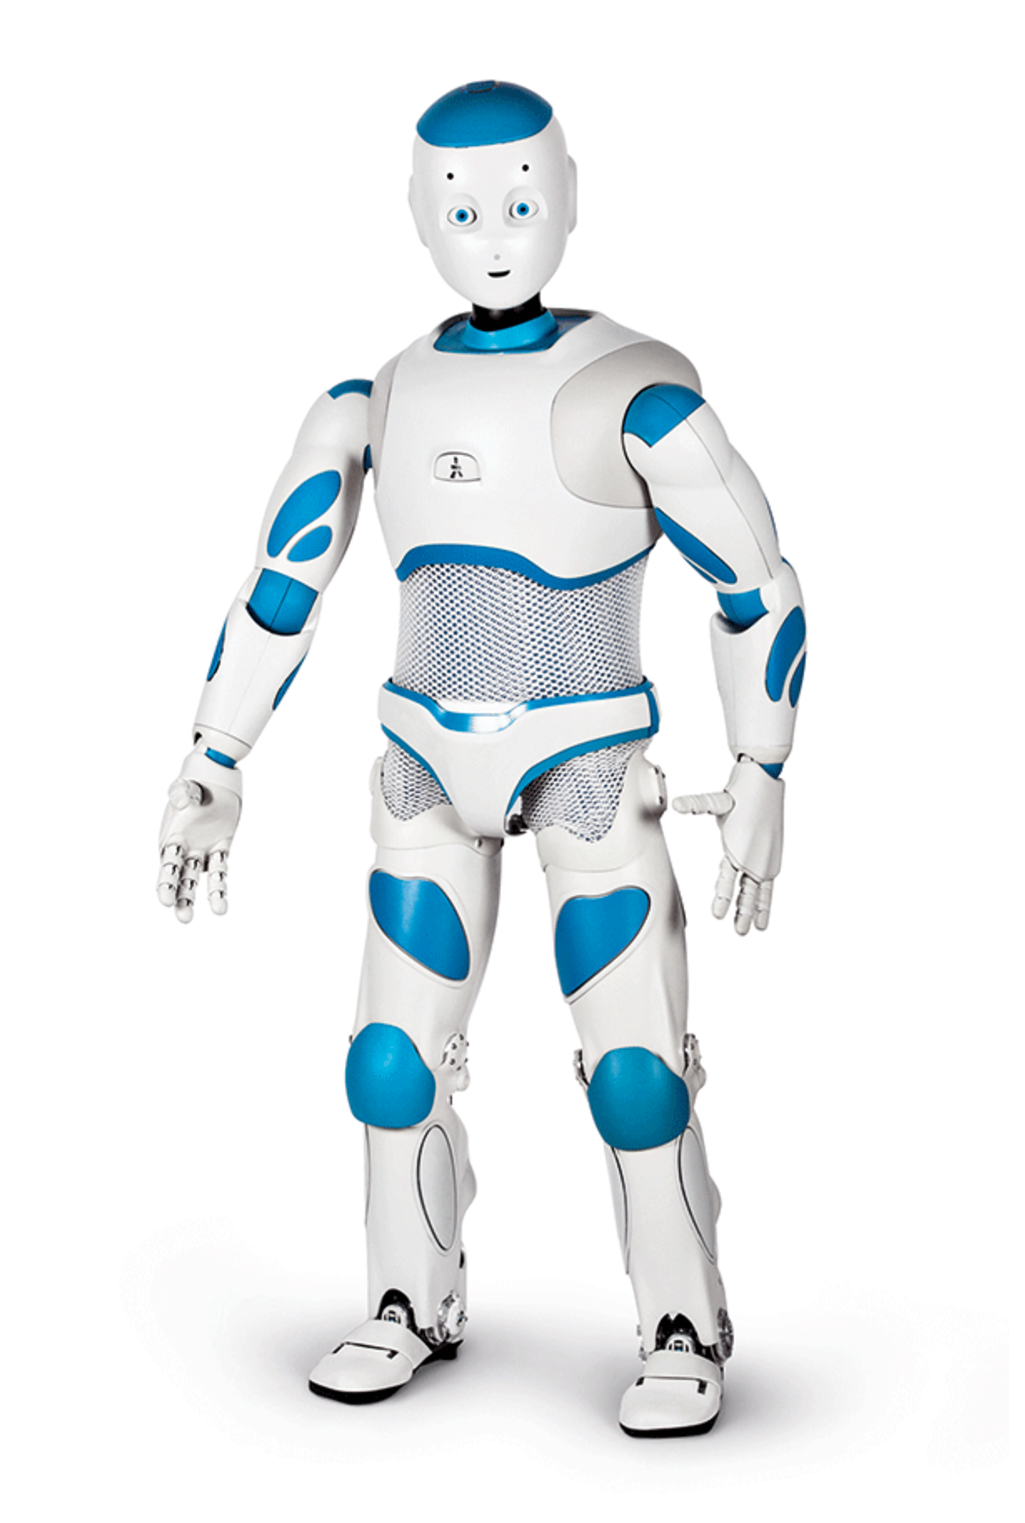
\includegraphics[width=0.35\textwidth]{images/Romeo.eps}
         \caption{Romeo robot \cite{Penton}}
\vspace{-40pt}
\end{wrapfigure}

A said previously, Romeo has the aim to help old people or people who has some kind of disability. Therefore, Romeo has been build with an structure which allows it to open doors, climb stairs and reach objects on a table. Moreover, it has several sensors which allow him to understand the environment and adapt him to it. Although, in order to make a good use of this hardware, it is necessary to complement it with a powerful software as is NAOqi.

%TODO
% Afegir mes coses

\subsection{Hardware}
\label{sec:romeo_hardware}

Because of the aim of this package, this section is focused on the hardware related to: (1) the arms, in order to do the grasp and (2) the 3D vision of the robot, due to the object recognition and positioning.

%Romeo is 1.4 m tall humanoid robot with 37 degrees of freedom:
%
%\begin{itemize}
%\item \textbf{Head} has 4 DoF.
%\item \textbf{Eyes} have 2 DoF for each eye.
%\item \textbf{Arms} have 7 DoF for each arm.
%\item \textbf{Legs} have 7 DoF for each leg.
%\item \textbf{Trunk} has 1 DoF.
%\end{itemize} 

\subsubsection{Romeo arms}

Each Romeo arm has 7 DoF plus 1 DoF to open and close the hand, so it has one redundancy for the movement of the arm. The links of the left arm are shown in Figure \ref{fig:romeo_arm}, the right arm is symmetric and changing the initial "L" or "l" to "R" or "r".

\begin{figure}[h]
\centering
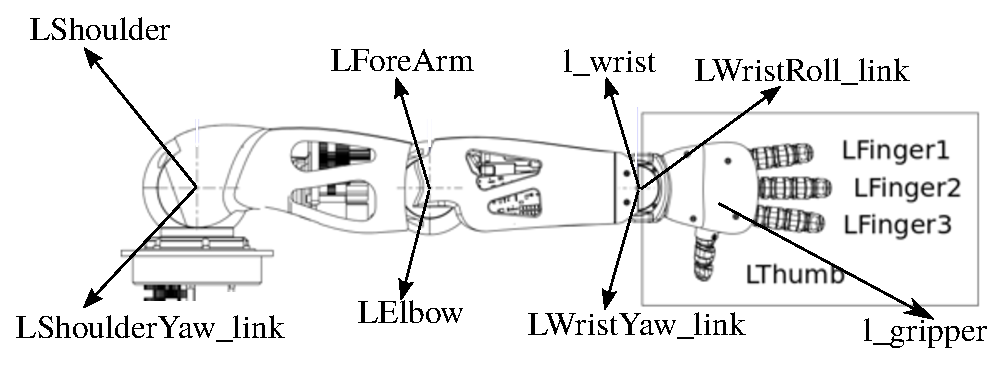
\includegraphics[width=0.8\textwidth]{images/arm_link.eps}
\caption{Links of Romeo left arm \cite{Aldebaran}\label{fig:romeo_arm}}
\end{figure}

Although, an arm can be seen as an entire group, in robotics is usually to split it in two groups: (1) the arm group which is the main part of the arm and (2) the end effector group which is the gripper with the joints that allow to interact with objects. In order to understand the tree of links-joints and the distribution of this groups in Romeo there is the Table \ref{tab:tree_group_links_joint} which shows the parent and child link of every joint and the group which it belongs. It should be stated that when is requested to move a group to a position, is used the position of the last link of the group. Furthermore, the \texttt{L$/$RHand} joint is special because it has the aim of open and close the hand moving all the fingers together. Moreover, there is a group for every arm, but not used any more, named \texttt{arm\_hand\_left} or \texttt{arm\_hand\_right} which takes all the joints and links of the arm and hand together.

\begin{table}[h]
\begin{center}
\begin{tabular}{|c|c|c|c|}
\hline
\multirow{2}{*}{\textbf{Group}} & \multirow{2}{*}{\textbf{Joint}} & \multicolumn{2}{|c|}{\textbf{Links}} \\ \cline{3-4}\noalign{\smallskip} &  & \textbf{Parent} & \textbf{Child} \\ \hline\noalign{\smallskip}
\multirow{6}{*}{left\_arm}
& LShoulderPitch & torso & LShoulder \\
& LShoulderYaw & LShoulder & LShoulderYaw\_link \\
& LElbowRoll & LShoulderYaw\_link & LForeArm \\
& LElbowYaw & LForeArm & LElbow \\                            
& LWristRoll & LElbow & LWristRoll\_link \\                   
& LWristYaw & LWristRoll\_link & LWristYaw\_link \\ \hline\noalign{\smallskip}
\multirow{2}{*}{left\_hand}
& LWristPitch & LWristYaw\_link & l\_wrist \\
& LHand & l\_wrist & l\_gripper \\ \hline
\end{tabular}
\caption{Joints of Romeo left arm with parent and child links\label{tab:tree_group_links_joint}}
\end{center}
\end{table}

\subsubsection{Romeo 3D vision hardware}

Romeo has several vision sensors: (1) one RGB camera on each eye; (2) two more fixes above each eye and (3) an optional ASUS Xtion on the cap. Therefore, Romeo is capable of having depth data with the RGB cameras, however, some functionalities are only available with the ASUS Xtion. When this 3D sensor is connected to the robot, all the functionalities that use depth data change the source and use the information from the Xtion camera. 

Referring to the ASUS Xtion camera, according to \cite{Aldebaran}, it has a color camera of 0.3 Mp and a depth camera up to 320x240 at 20 fps. Besides, the focus range is from 80 cm to 3.5 m and the field of view is 58º in horizontal and 45º in vertical.

\subsection{NAOqi}
\label{sec:naoqi}

NAOqi is the name of the main software that runs on the robots control it. The NAOqi framework is \texttt{Cross plataform} and \texttt{Cross language}. Therefore, it is possible to develop in Windows, Linux or Mac and using C++ or Python. Although, below it is only explained a brief description about NAOqi proxies and NAOqi modules, more information about the framework can be found at \citep{Aldebaran}. 

On one hand, the NAOqi modules are classes within libraries that contain various methods. Every module has a particular subject which it is controlling. On the other hand, the NAOqi proxies is an object that has the behaviour of the NAOqi module that represents. Therefore, the proxy from a module contain the methods of the pertinent module.

Because of the aim of this project there are four main modules:

\begin{itemize}
\item \texttt{ALMemory} which handle all the key information related to the hardware configuration
\item \texttt{DCM} in charge of the communication with almost every electronic device in the robot except sound and cameras.
\item \texttt{ALMotion} in charge of the movement of the robot
\item \texttt{ALVideoDevice} which provides images from the video sources in an efficient way.
\end{itemize} 

Below is explained the most important things about this modules just to have an idea and to be able to understand the following Section \ref{sec:romeo_ros}.

\subsubsection{DCM}

Firstly, the DCM module, it is the link between NAOqi modules and the software in electronic boards. Therefore, modules like ALMotion use the DCM to send commands to Actuators, and also get sensor information returned by the DCM in ALMemory. Therefore, using directly DCM commands to control the robot is faster and more efficient, but is more difficult to use than the NAOqi modules. An overview of how the DCM works can be seen in Figure \ref{fig:naoqi_DCM}.

\begin{figure}[h]
\centering
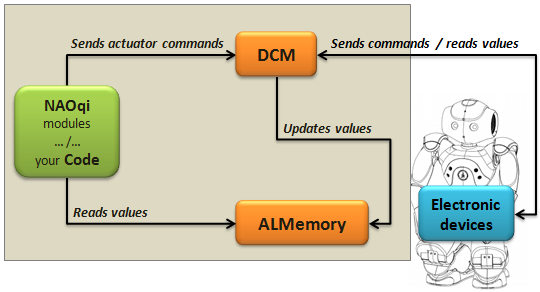
\includegraphics[width=0.8\textwidth]{images/dcm_overview.png}
\caption{Behaviour of DCM module \cite{Aldebaran}\label{fig:naoqi_DCM}}
\end{figure}

\subsubsection{ALMotion}

Secondly, the ALMotion module, it can do both get information from joints and set specific angles or trajectories. Some of the most important functions, at least for this work, are the following ones:

\begin{itemize}
\item \texttt{getStiffness()} and \texttt{setStiffness} to get or set the values of stiffness to one or more joints.
\item \texttt{getAngles()} and \texttt{setAngles} to get or set the angle to one or more joints. Moreover, can set for every joint the fraction of maximum speed use to reach the specific angle.
\item \texttt{angleInterpolation()} to set an interpolated trajectory for one or more joints, given the angles for specific moments. 
\end{itemize}

\subsubsection{ALVideoDevice}

Finally, the ALVideoDevice module, it allows the package to get images from the sources available from the robot. As said in Section \ref{sec:romeo_hardware}, there are several cameras, so the images from one or other camera can be got depending on the camera index. For this module, there are two main functions:

\begin{itemize}
\item \texttt{subscribeCamera()} given the features of the desired image (source, resolution, colorspace and fps) returns the string handle which identify the subscriber.
\item \texttt{getImageRemote()} given the string handle returns the container of the latest image from the video source.
\end{itemize}


\section{Software required}
%TODO
%Introduction of software required

\subsection{ROS (Robotic Operative System)}
\label{sec:ROS}

\textit{\textbf{R}obot \textbf{O}perating \textbf{S}ystem} \cite{ROS} is an open-source and flexible framework to develop robot software. There are five main elements in this framework: (1) nodes which are the process; (2) messages that are used for the communication between nodes; (3) topics that is where the message is published by the node; (4) services is the where the node have to send a request message to get a response message and (5) actions which are like a service but can send a feedback while the activity is not still done. ROS allow the communication between process in two different ways: (1) publisher/subscriber system and using services. 

\begin{enumerate}
\item Publisher/subscriber system is anonymous and asynchronous. Moreover, can be more than one publisher and/or subscriber for an unique topic.
\item Services are defined by two messages: (1) request message from the node and (2) response message. Therefore, the response message is given by the node which allocate the service depending on the information given in the request message. 
\end{enumerate}

Although, the main aim is to be able to reuse the code yet develop in robotics investigations. Also the philosophical goals of ROS can be summarized \cite{Quigley}: (1) Peer-to-Peer, (2) tools-based, (3) multi-lingual, (4) thin, (5) free and open-source. 

ROS is a required software for \texttt{romeo\_grasper} because this is the framework used to communicate the process in charge with the different devices and Romeo. Therefore, it is needed for the robot and for every device a way to communicate with ROS.

\subsection{Ros packages for Romeo}
\label{sec:romeo_ros}

Aldebaran company has created some packages to communicate Romeo, Nao and Pepper with ROS. At this stage are only explained some which are related with Romeo, but some of them are used also for Nao and Pepper. Although, these packages are open-source, so are continuously improving them by the community, but before the changes are released as oficial, their are revised by experimented developers on Romeo.

On one hand, there are the packages used for the three robots that are in the \texttt{ros-naoqi} repository \cite{ros-naoqi}:
\begin{itemize}
\item \texttt{naoqi\_bridge} metapackage which include the following packages:
\begin{itemize}
\item \texttt{naoqi\_driver\_py} Python code in charge of getting data from joints.
\item \texttt{naoqi\_pose} which handle the movement of the robot.
\item \texttt{naoqi\_sensor\_py} get the information from sensors as camera, contact sensors, microphone and sonar.
\item \texttt{naoqi\_tools} allow to generate and modify Aldebaran's robot models easily.
\end{itemize}
\item \texttt{naoqi\_dirver} another version of \texttt{naoqi\_driver\_py} in C++, but less developed 
\item \texttt{naoqi\_bridge\_msgs} contains all the needed messages, services and actions to use the naoqi packages.
\end{itemize}

On the other hand, the packages used from \texttt{ros-aldebaran} repository \cite{ros-aldebaran} are the following:

\begin{itemize}
\item \texttt{romeo\_robot} metapackage which include the following packages:
\begin{itemize}
\item \texttt{romeo\_bringup} used to launch the essentials nodes of the metapackage.
\item \texttt{romeo\_dcm} which handle the communication with the Romeo electronic devices.
\item \texttt{romeo\_description} contains the model of the robot in different type of files
\item \texttt{romeo\_sensors\_py} add the depth camera and reuse \texttt{naoqi\_sensor\_py}.
\end{itemize}
\item \texttt{romeo\_moveit\_config} explained in Section \ref{sec:romeo_moveit_config}.
\item \texttt{romeo\_moveit\_actions} explained in Section \ref{sec:romeo_moveit_actions}.
\end{itemize}

As described in Section \ref{sec:naoqi}, NAOqi proxies are used to connect to a NAOqi module. Therefore, the base of all these packages is to create the pertinent proxies to send data to NAOqi or to get data from NAOqi and then publish it on ROS. This way of working is shown in Figure \ref{fig:Romeo-ROS}. Below are explained the most important packages to work with \texttt{romeo\_grasper} package.

\begin{figure}[h]
\centering
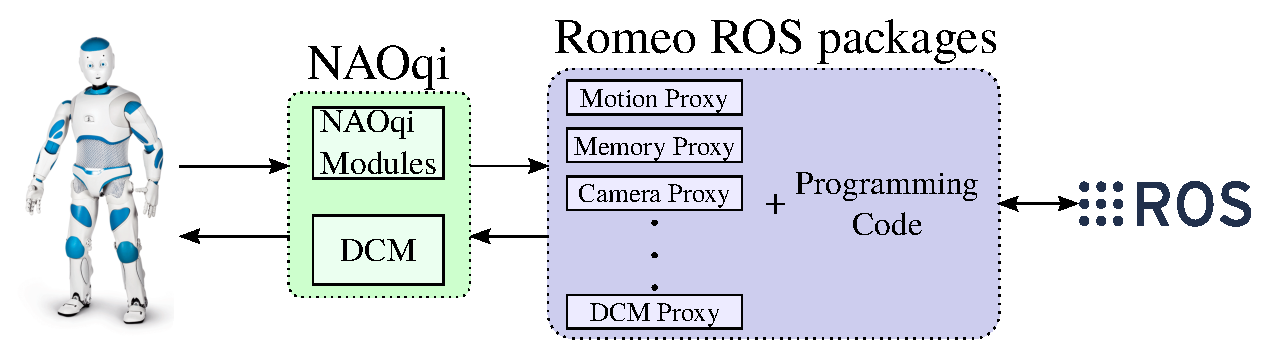
\includegraphics[width=0.85\textwidth]{images/Romeo-ROS.eps}
\caption{Communication between Romeo and ROS\label{fig:Romeo-ROS}}
\end{figure}

\subsubsection{NAOqi driver}

As said previously, there are two different NAOqi driver packages: (1) \texttt{naoqi\_driver\_py} and (2) \texttt{naoqi\_driver}. Due to unknown reason \texttt{naoqi\_driver\_py} is more developed than \texttt{naoqi\_driver}, so it is better to work with the first one. In order to get the information from the robot joints, this package is connected to ALMotion module. Then, it gets and publish this data to ROS with a frequency of 25 Hz. As shown in Figure \ref{fig:naoqi_driver}, the topics where it is published are \texttt{$/$joint\_states} and \texttt{$/$joint\_stiffness}.

\begin{figure}[h]
\centering
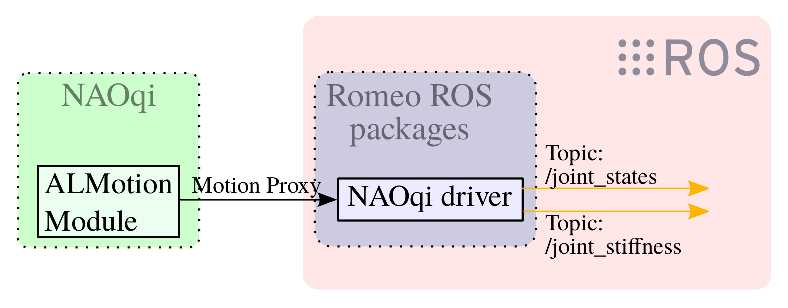
\includegraphics[width=0.8\textwidth]{images/naoqi_driver.eps}
\caption{Overview NAOqi driver package\label{fig:naoqi_driver}}
\end{figure}

\subsubsection{NAOqi pose}

Although, this package uses two nodes: (1) pose controller node and (2) pose manager node; only pose controller node is important for \texttt{romeo\_grasper}. Whereas the pose controller node is in charge of sending the goal angle or goal trajectory to the joints, pose manager only is used to move the joints to a predefined posture. Therefore, below is only explained the pose controller node.

Therefore, using the motion proxy it sends the pertinent commands to ALMotion module depending on from where the pose controller node take the information. There are several ways to communicate with this node, as can be seen in Figure \ref{fig:pose_controller}. Among these, the one used in \texttt{romeo\_grasper} is the action \texttt{$/$joint\_trajectory}. In order to run this action the request message has to contain the angles of the joint for each specific time from start. Then, the ALMotion function \texttt{angleInterpolation} is run in another thread and when the action is done it sends the final joint state.

%\begin{itemize}
%\item \textbf{Topics} 
%\begin{itemize}
%\item \texttt{$/$joint\_angles} which set the joints named in the message to a specific angle and go there with a specific factor of the maximum speed for the joint.
%\item \texttt{$/$joint\_stiffness} which set the stiffness of the named joints to a value.
%\end{itemize}
%\item \textbf{Services}
%\begin{itemize}
%\item \texttt{$/$wake\_up}
%\end{itemize}
%\end{itemize}

\begin{figure}[h]
\centering
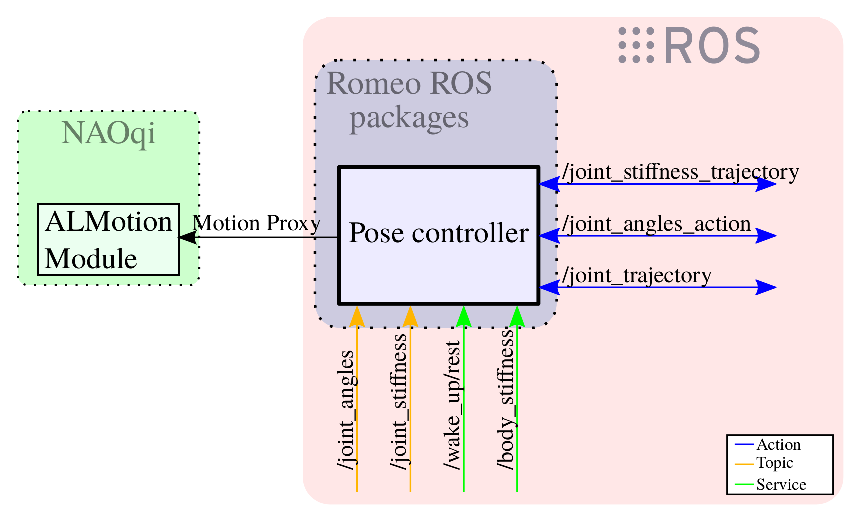
\includegraphics[width=0.8\textwidth]{images/pose_controller.eps}
\caption{Overview Pose controller node\label{fig:pose_controller}}
\end{figure}

\subsubsection{DCM driver}

Although, previously is said that the DCM handle the communication with the Romeo electronic devices, till the moment of writing this, the code developed only implements the communication with the Romeo joints to set the pertinent angle at the precise moment. Despite the fact that the \texttt{naoqi\_pose} can also do this, using DCM is more efficient and more direct, as explained in Section \ref{sec:naoqi}.

In robotics is needed to make a realtime control of the joints, in this case to do that is used \texttt{controller manager} from the \texttt{ROS Control} metapackage. Therefore, when someone or a package wants to send commands through DCM should communicate with \texttt{controller manager} and then this send the commands to \texttt{DCM driver} in the right way to have realtime control. An overview of this communication is shown in Figure \ref{fig:dcm_driver}. Moreover, in Figure \ref{fig:dcm_driver_flow} can be seen how it works this package.

\begin{figure}[h]
\centering
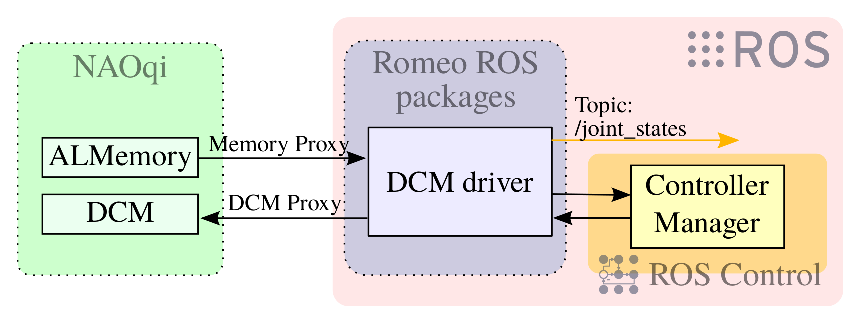
\includegraphics[width=0.8\textwidth]{images/dcm_driver.eps}
\caption{Overview Romeo DCM package\label{fig:dcm_driver}}
\end{figure}

\begin{figure}[h]
\centering
% Graphic for TeX using PGF
% Title: /home/lluis/Escritorio/TFM/Informe/images/dcm_driver_flow.dia
% Creator: Dia v0.97.2
% CreationDate: Sat May 28 14:20:42 2016
% For: lluis
% \usepackage{tikz}
% The following commands are not supported in PSTricks at present
% We define them conditionally, so when they are implemented,
% this pgf file will use them.
\ifx\du\undefined
  \newlength{\du}
\fi
\setlength{\du}{15\unitlength}
\begin{tikzpicture}
\pgftransformxscale{1.000000}
\pgftransformyscale{-1.000000}
\definecolor{dialinecolor}{rgb}{0.000000, 0.000000, 0.000000}
\pgfsetstrokecolor{dialinecolor}
\definecolor{dialinecolor}{rgb}{1.000000, 1.000000, 1.000000}
\pgfsetfillcolor{dialinecolor}
\definecolor{dialinecolor}{rgb}{0.678431, 0.847059, 0.901961}
\pgfsetfillcolor{dialinecolor}
\fill (17.445000\du,4.450000\du)--(17.445000\du,6.350000\du)--(24.795124\du,6.350000\du)--(24.795124\du,4.450000\du)--cycle;
\pgfsetlinewidth{0.100000\du}
\pgfsetdash{}{0pt}
\pgfsetdash{}{0pt}
\pgfsetmiterjoin
\definecolor{dialinecolor}{rgb}{0.000000, 0.000000, 0.000000}
\pgfsetstrokecolor{dialinecolor}
\draw (17.445000\du,4.450000\du)--(17.445000\du,6.350000\du)--(24.795124\du,6.350000\du)--(24.795124\du,4.450000\du)--cycle;
% setfont left to latex
\definecolor{dialinecolor}{rgb}{0.000000, 0.000000, 0.000000}
\pgfsetstrokecolor{dialinecolor}
\node at (21.120062\du,5.595000\du){Launch DCM driver};
\definecolor{dialinecolor}{rgb}{0.678431, 0.847059, 0.901961}
\pgfsetfillcolor{dialinecolor}
\fill (15.976200\du,11.200000\du)--(15.976200\du,13.900000\du)--(26.281575\du,13.900000\du)--(26.281575\du,11.200000\du)--cycle;
\pgfsetlinewidth{0.100000\du}
\pgfsetdash{}{0pt}
\pgfsetdash{}{0pt}
\pgfsetmiterjoin
\definecolor{dialinecolor}{rgb}{0.000000, 0.000000, 0.000000}
\pgfsetstrokecolor{dialinecolor}
\draw (15.976200\du,11.200000\du)--(15.976200\du,13.900000\du)--(26.281575\du,13.900000\du)--(26.281575\du,11.200000\du)--cycle;
% setfont left to latex
\definecolor{dialinecolor}{rgb}{0.000000, 0.000000, 0.000000}
\pgfsetstrokecolor{dialinecolor}
\node at (21.128888\du,12.345000\du){Initialize Controller Manager};
% setfont left to latex
\definecolor{dialinecolor}{rgb}{0.000000, 0.000000, 0.000000}
\pgfsetstrokecolor{dialinecolor}
\node at (21.128888\du,13.145000\du){with the controled joints};
\definecolor{dialinecolor}{rgb}{0.678431, 0.847059, 0.901961}
\pgfsetfillcolor{dialinecolor}
\fill (16.090000\du,7.400000\du)--(16.090000\du,10.100000\du)--(26.132975\du,10.100000\du)--(26.132975\du,7.400000\du)--cycle;
\pgfsetlinewidth{0.100000\du}
\pgfsetdash{}{0pt}
\pgfsetdash{}{0pt}
\pgfsetmiterjoin
\definecolor{dialinecolor}{rgb}{0.000000, 0.000000, 0.000000}
\pgfsetstrokecolor{dialinecolor}
\draw (16.090000\du,7.400000\du)--(16.090000\du,10.100000\du)--(26.132975\du,10.100000\du)--(26.132975\du,7.400000\du)--cycle;
% setfont left to latex
\definecolor{dialinecolor}{rgb}{0.000000, 0.000000, 0.000000}
\pgfsetstrokecolor{dialinecolor}
\node at (21.111488\du,8.545000\du){Load params from ROS and};
% setfont left to latex
\definecolor{dialinecolor}{rgb}{0.000000, 0.000000, 0.000000}
\pgfsetstrokecolor{dialinecolor}
\node at (21.111488\du,9.345000\du){connect to Romeo proxies};
\pgfsetlinewidth{0.100000\du}
\pgfsetdash{}{0pt}
\pgfsetdash{}{0pt}
\pgfsetbuttcap
\pgfsetmiterjoin
\pgfsetlinewidth{0.100000\du}
\pgfsetbuttcap
\pgfsetmiterjoin
\pgfsetdash{}{0pt}
\definecolor{dialinecolor}{rgb}{1.000000, 0.878431, 0.650980}
\pgfsetfillcolor{dialinecolor}
\pgfpathmoveto{\pgfpoint{31.247538\du}{2.500000\du}}
\pgfpathlineto{\pgfpoint{36.735038\du}{2.500000\du}}
\pgfpathlineto{\pgfpoint{37.832538\du}{3.500000\du}}
\pgfpathlineto{\pgfpoint{36.735038\du}{4.500000\du}}
\pgfpathlineto{\pgfpoint{31.247538\du}{4.500000\du}}
\pgfpathlineto{\pgfpoint{30.150038\du}{3.500000\du}}
\pgfpathlineto{\pgfpoint{31.247538\du}{2.500000\du}}
\pgfusepath{fill}
\definecolor{dialinecolor}{rgb}{0.000000, 0.000000, 0.000000}
\pgfsetstrokecolor{dialinecolor}
\pgfpathmoveto{\pgfpoint{31.247538\du}{2.500000\du}}
\pgfpathlineto{\pgfpoint{36.735038\du}{2.500000\du}}
\pgfpathlineto{\pgfpoint{37.832538\du}{3.500000\du}}
\pgfpathlineto{\pgfpoint{36.735038\du}{4.500000\du}}
\pgfpathlineto{\pgfpoint{31.247538\du}{4.500000\du}}
\pgfpathlineto{\pgfpoint{30.150038\du}{3.500000\du}}
\pgfpathlineto{\pgfpoint{31.247538\du}{2.500000\du}}
\pgfusepath{stroke}
% setfont left to latex
\definecolor{dialinecolor}{rgb}{0.000000, 0.000000, 0.000000}
\pgfsetstrokecolor{dialinecolor}
\node at (33.991288\du,3.700000\du){While ROS is OK};
\definecolor{dialinecolor}{rgb}{0.678431, 0.847059, 0.901961}
\pgfsetfillcolor{dialinecolor}
\fill (28.778607\du,5.400000\du)--(28.778607\du,7.300000\du)--(39.203968\du,7.300000\du)--(39.203968\du,5.400000\du)--cycle;
\pgfsetlinewidth{0.100000\du}
\pgfsetdash{}{0pt}
\pgfsetdash{}{0pt}
\pgfsetmiterjoin
\definecolor{dialinecolor}{rgb}{0.000000, 0.000000, 0.000000}
\pgfsetstrokecolor{dialinecolor}
\draw (28.778607\du,5.400000\du)--(28.778607\du,7.300000\du)--(39.203968\du,7.300000\du)--(39.203968\du,5.400000\du)--cycle;
% setfont left to latex
\definecolor{dialinecolor}{rgb}{0.000000, 0.000000, 0.000000}
\pgfsetstrokecolor{dialinecolor}
\node at (33.991288\du,6.545000\du){Read Joints from ALMemory};
\definecolor{dialinecolor}{rgb}{0.678431, 0.847059, 0.901961}
\pgfsetfillcolor{dialinecolor}
\fill (28.766960\du,8.400000\du)--(28.766960\du,10.300000\du)--(39.215616\du,10.300000\du)--(39.215616\du,8.400000\du)--cycle;
\pgfsetlinewidth{0.100000\du}
\pgfsetdash{}{0pt}
\pgfsetdash{}{0pt}
\pgfsetmiterjoin
\definecolor{dialinecolor}{rgb}{0.000000, 0.000000, 0.000000}
\pgfsetstrokecolor{dialinecolor}
\draw (28.766960\du,8.400000\du)--(28.766960\du,10.300000\du)--(39.215616\du,10.300000\du)--(39.215616\du,8.400000\du)--cycle;
% setfont left to latex
\definecolor{dialinecolor}{rgb}{0.000000, 0.000000, 0.000000}
\pgfsetstrokecolor{dialinecolor}
\node at (33.991288\du,9.545000\du){Update Controller Manager};
\definecolor{dialinecolor}{rgb}{0.678431, 0.847059, 0.901961}
\pgfsetfillcolor{dialinecolor}
\fill (28.231794\du,11.350000\du)--(28.231794\du,13.250000\du)--(39.750782\du,13.250000\du)--(39.750782\du,11.350000\du)--cycle;
\pgfsetlinewidth{0.100000\du}
\pgfsetdash{}{0pt}
\pgfsetdash{}{0pt}
\pgfsetmiterjoin
\definecolor{dialinecolor}{rgb}{0.000000, 0.000000, 0.000000}
\pgfsetstrokecolor{dialinecolor}
\draw (28.231794\du,11.350000\du)--(28.231794\du,13.250000\du)--(39.750782\du,13.250000\du)--(39.750782\du,11.350000\du)--cycle;
% setfont left to latex
\definecolor{dialinecolor}{rgb}{0.000000, 0.000000, 0.000000}
\pgfsetstrokecolor{dialinecolor}
\node at (33.991288\du,12.495000\du){Send commands to DCM proxy};
\definecolor{dialinecolor}{rgb}{0.631373, 0.862745, 0.631373}
\pgfsetfillcolor{dialinecolor}
\fill (29.591816\du,14.250000\du)--(29.591816\du,16.150000\du)--(38.390760\du,16.150000\du)--(38.390760\du,14.250000\du)--cycle;
\pgfsetlinewidth{0.100000\du}
\pgfsetdash{}{0pt}
\pgfsetdash{}{0pt}
\pgfsetmiterjoin
\definecolor{dialinecolor}{rgb}{0.000000, 0.000000, 0.000000}
\pgfsetstrokecolor{dialinecolor}
\draw (29.591816\du,14.250000\du)--(29.591816\du,16.150000\du)--(38.390760\du,16.150000\du)--(38.390760\du,14.250000\du)--cycle;
% setfont left to latex
\definecolor{dialinecolor}{rgb}{0.000000, 0.000000, 0.000000}
\pgfsetstrokecolor{dialinecolor}
\node at (33.991288\du,15.395000\du){Publish in /joint\_states};
\pgfsetlinewidth{0.100000\du}
\pgfsetdash{}{0pt}
\pgfsetdash{}{0pt}
\pgfsetmiterjoin
\pgfsetbuttcap
{
\definecolor{dialinecolor}{rgb}{0.000000, 0.000000, 0.000000}
\pgfsetfillcolor{dialinecolor}
% was here!!!
\pgfsetarrowsend{stealth}
{\pgfsetcornersarced{\pgfpoint{0.000000\du}{0.000000\du}}\definecolor{dialinecolor}{rgb}{0.000000, 0.000000, 0.000000}
\pgfsetstrokecolor{dialinecolor}
\draw (21.128900\du,13.900000\du)--(21.128900\du,14.950000\du)--(26.885078\du,14.950000\du)--(26.885078\du,1.450000\du)--(33.991288\du,1.450000\du)--(33.991288\du,2.500000\du);
}}
\pgfsetlinewidth{0.100000\du}
\pgfsetdash{}{0pt}
\pgfsetdash{}{0pt}
\pgfsetmiterjoin
\pgfsetbuttcap
{
\definecolor{dialinecolor}{rgb}{0.000000, 0.000000, 0.000000}
\pgfsetfillcolor{dialinecolor}
% was here!!!
\pgfsetarrowsend{stealth}
{\pgfsetcornersarced{\pgfpoint{0.000000\du}{0.000000\du}}\definecolor{dialinecolor}{rgb}{0.000000, 0.000000, 0.000000}
\pgfsetstrokecolor{dialinecolor}
\draw (33.991288\du,16.150000\du)--(33.991288\du,16.525544\du)--(27.768018\du,16.525544\du)--(27.768018\du,3.500000\du)--(30.150038\du,3.500000\du);
}}
\pgfsetlinewidth{0.100000\du}
\pgfsetdash{}{0pt}
\pgfsetdash{}{0pt}
\pgfsetbuttcap
{
\definecolor{dialinecolor}{rgb}{0.000000, 0.000000, 0.000000}
\pgfsetfillcolor{dialinecolor}
% was here!!!
\pgfsetarrowsend{stealth}
\definecolor{dialinecolor}{rgb}{0.000000, 0.000000, 0.000000}
\pgfsetstrokecolor{dialinecolor}
\draw (33.991288\du,4.500000\du)--(33.991288\du,5.400000\du);
}
\pgfsetlinewidth{0.100000\du}
\pgfsetdash{}{0pt}
\pgfsetdash{}{0pt}
\pgfsetbuttcap
{
\definecolor{dialinecolor}{rgb}{0.000000, 0.000000, 0.000000}
\pgfsetfillcolor{dialinecolor}
% was here!!!
\pgfsetarrowsend{stealth}
\definecolor{dialinecolor}{rgb}{0.000000, 0.000000, 0.000000}
\pgfsetstrokecolor{dialinecolor}
\draw (33.991288\du,7.300000\du)--(33.991288\du,8.400000\du);
}
\pgfsetlinewidth{0.100000\du}
\pgfsetdash{}{0pt}
\pgfsetdash{}{0pt}
\pgfsetbuttcap
{
\definecolor{dialinecolor}{rgb}{0.000000, 0.000000, 0.000000}
\pgfsetfillcolor{dialinecolor}
% was here!!!
\pgfsetarrowsend{stealth}
\definecolor{dialinecolor}{rgb}{0.000000, 0.000000, 0.000000}
\pgfsetstrokecolor{dialinecolor}
\draw (33.991288\du,10.300000\du)--(33.991288\du,11.350000\du);
}
\pgfsetlinewidth{0.100000\du}
\pgfsetdash{}{0pt}
\pgfsetdash{}{0pt}
\pgfsetbuttcap
{
\definecolor{dialinecolor}{rgb}{0.000000, 0.000000, 0.000000}
\pgfsetfillcolor{dialinecolor}
% was here!!!
\pgfsetarrowsend{stealth}
\definecolor{dialinecolor}{rgb}{0.000000, 0.000000, 0.000000}
\pgfsetstrokecolor{dialinecolor}
\draw (33.991288\du,13.250000\du)--(33.991288\du,14.250000\du);
}
\pgfsetlinewidth{0.100000\du}
\pgfsetdash{}{0pt}
\pgfsetdash{}{0pt}
\pgfsetbuttcap
{
\definecolor{dialinecolor}{rgb}{0.000000, 0.000000, 0.000000}
\pgfsetfillcolor{dialinecolor}
% was here!!!
\pgfsetarrowsend{stealth}
\definecolor{dialinecolor}{rgb}{0.000000, 0.000000, 0.000000}
\pgfsetstrokecolor{dialinecolor}
\draw (21.120100\du,6.350000\du)--(21.111500\du,7.400000\du);
}
\pgfsetlinewidth{0.100000\du}
\pgfsetdash{}{0pt}
\pgfsetdash{}{0pt}
\pgfsetbuttcap
{
\definecolor{dialinecolor}{rgb}{0.000000, 0.000000, 0.000000}
\pgfsetfillcolor{dialinecolor}
% was here!!!
\pgfsetarrowsend{stealth}
\definecolor{dialinecolor}{rgb}{0.000000, 0.000000, 0.000000}
\pgfsetstrokecolor{dialinecolor}
\draw (21.111500\du,10.100000\du)--(21.128900\du,11.200000\du);
}
\pgfsetlinewidth{0.100000\du}
\pgfsetdash{}{0pt}
\pgfsetdash{}{0pt}
\pgfsetbuttcap
\pgfsetmiterjoin
\pgfsetlinewidth{0.100000\du}
\pgfsetbuttcap
\pgfsetmiterjoin
\pgfsetdash{}{0pt}
\definecolor{dialinecolor}{rgb}{0.000000, 0.000000, 0.000000}
\pgfsetstrokecolor{dialinecolor}
\draw (15.189518\du,8.171050\du)--(15.189518\du,9.328945\du);
\pgfsetbuttcap
\pgfsetmiterjoin
\pgfsetdash{}{0pt}
\definecolor{dialinecolor}{rgb}{0.000000, 0.000000, 0.000000}
\pgfsetstrokecolor{dialinecolor}
\draw (15.189518\du,8.171050\du)--(9.376360\du,8.171050\du);
\pgfsetbuttcap
\pgfsetmiterjoin
\pgfsetdash{}{0pt}
\definecolor{dialinecolor}{rgb}{0.000000, 0.000000, 0.000000}
\pgfsetstrokecolor{dialinecolor}
\draw (15.189518\du,9.328945\du)--(9.376360\du,9.328945\du);
% setfont left to latex
\definecolor{dialinecolor}{rgb}{0.000000, 0.000000, 0.000000}
\pgfsetstrokecolor{dialinecolor}
\node at (12.137610\du,8.978945\du){ROS Parameters};
\pgfsetlinewidth{0.100000\du}
\pgfsetdash{}{0pt}
\pgfsetdash{}{0pt}
\pgfsetbuttcap
{
\definecolor{dialinecolor}{rgb}{0.000000, 0.000000, 0.000000}
\pgfsetfillcolor{dialinecolor}
% was here!!!
\pgfsetarrowsend{stealth}
\definecolor{dialinecolor}{rgb}{0.000000, 0.000000, 0.000000}
\pgfsetstrokecolor{dialinecolor}
\draw (15.189518\du,8.749997\du)--(16.090000\du,8.750000\du);
}
\end{tikzpicture}

\caption{Flow sequence of Romeo DCM package\label{fig:dcm_driver_flow}}
\end{figure}

\subsubsection{Romeo sensor}
%Pensar amb si talvegada desconectant sa Xtion vagi més bé treient la info a partir de les cameres RGB.

%La camera de l'esquerra a dalt esta considerada com a camera bottom i sa de la dreta dalt es com a front

%TODO
%TEST!! change encoding mono16 for 16UC1
Because of \texttt{romeo\_sensor\_py} is an addition of \texttt{naoqi\_sensor\_py}, it should be understood how works this last one. Firstly, initialize the ROS publishers and the camera proxy. Secondly, it gets and applies the camera parameters. After that, the function \texttt{subscribeCamera} is used to then can get the image container. Finally, it transforms all the received data to image messages to publish in the pertinent ROS topic. 

In order to add the depth camera is used the same code structure as in \texttt{naoqi\_sensor\_py}, but changing the camera index and adapting the image type to ROS. Unfortunately, it seems that this part is not well implemented, because at least with the test done here it gets a dark image, this fact is shown in Figure \ref{fig:ros_dark_depth_image}.  

\begin{figure}[h]
\begin{subfigure}[r]{0.48\textwidth}
\centering
		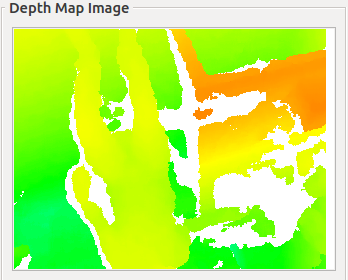
\includegraphics[width=\textwidth]{images/depth_camera_monitor.png}
        \caption{Image from Monitor, which is Aldebaran official program to see the what are the cameras recording.}
\end{subfigure}
~
\begin{subfigure}[r]{0.48\textwidth}
\centering
		
\includegraphics[width=\textwidth]{images/depth_camera_ROS.jpg}
        \caption{Image from the topic where \texttt{romeo\_sensor} publish.}
\end{subfigure}
\caption{Comparative images from the depth camera.\label{fig:ros_dark_depth_image}}
\end{figure}

Looking in the code one tested idea to solve it has been to change the camera index which currently is 2 (names \texttt{kDepthCamera}) which, according to \citep{Aldebaran}, to connect to ASUS Xtion should be 4 (named \texttt{kXTION}). After a lot of tests, changing the encoding and other features, it hasn't reach any good result. 

\subsection{V4R (Vision for Robots)}
\label{sec:V4R}

The V4R software is only a branch of a huge project named STRANDS \cite{strands} which has the aim to enable a robot to achieve robust and intelligent behaviour in human environments through adaptation to, and the exploitation of, long-term experience. Specifically V4R has the aim to provide the robot with life-long acquisition of object knowledge, incrementally extending its expertise over time.

In order to achieve this goal, V4R has several modules and apps going in that direction. Concerning to this project, two of the features which are the most interesting: (1) RGB-D object modelling for object recognition and tracking and (2) real-time object pose tracking.

On one hand, V4R has RTM-Toolbox (Recognition, Tracking and Modelling Object) \cite{Prankl2015} which includes a flexible system to reconstruct 3D models of objects captured with an RGB-D sensor. A major advantage of the method is that unlike  other modelling tools, this reconstruction pipeline allows  the user to acquire a full 3D model of the object. This is  achieved by acquiring several partial 3D models in different sessions that are automatically merged together to reconstruct a full 3D model. 

On the other hand, the real-time object pose tracking \cite{Prankl2013} \cite{Aldoma2013}, combines complementary interest points, for textured objects and for uniformly colored objects, in a common tracking framework which allows to handle a broad variety of objects regardless of their appearance and shape. Then, the point cloud around the detected object is analysed to confirm that the depth of the object is the right one.

Although, the V4R library is independent from ROS, there are wrappers for ROS \cite{gitV4RWrappers}. Therefore, the features described above can be used though ROS. However, there are some limitations. Even using a RGB-D sensor, to run RTM-Toolbox is necessary to have the sensor launched though OpenNi. The problem appears with some RGB-D cameras that are not supported by OpenNi like the Intel RealSense.\footnote{Installation of the camera drivers explained in Appendix \ref{app:camera_instal}} Therefore, it cannot use the RTM-Toolbox and only can use the modelling application the Microsoft Kinect and ASUS Xtion cameras. Except for this, in all the others features is possible to use any camera which can publish PointsClouds in a topic, see Figure \ref{fig:V4R-ROS}.

\begin{figure}[h]
\centering
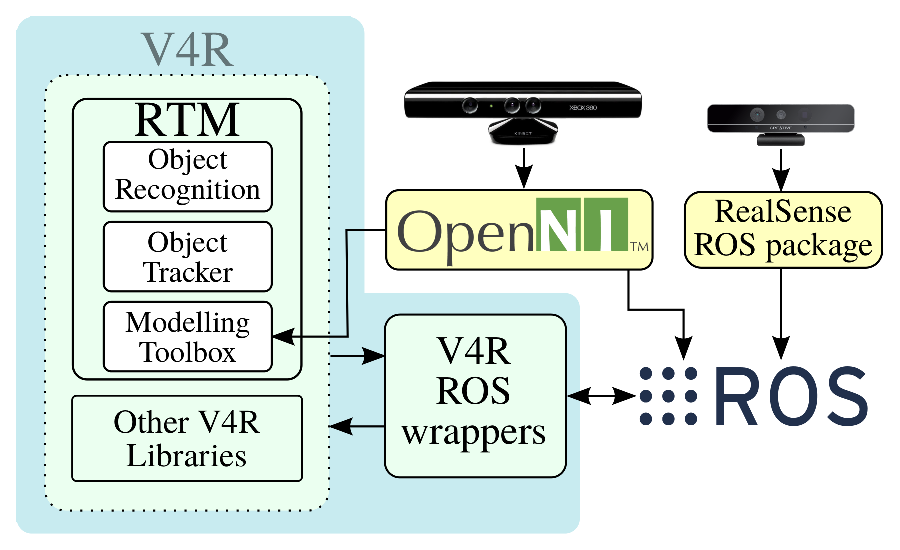
\includegraphics[width=0.8\textwidth]{images/V4R-ROS.eps}
\caption{Communication between V4R - ROS - Cameras RGB-D\label{fig:V4R-ROS}}
\end{figure}

\vspace{-5pt}
In order to use the toolbox and the tracker in \cite{gitV4RWrappers} is explained the instructions to install and a brief tutorial. However, it is good to add some information. Firstly, the way to be able to make a full 3D model of an object, for this is needed to use the multi-session modelling as explained in \cite{Prankl2015b}. Secondly, If the object itself is texture-less, the software relies on background texture in order to  successfully  model  these  kind  of  objects. So a good option is to add a textured sheet of paper on the supporting surface. Thirdly, the origin of the modeled object is posed automatically by the toolbox, so probably is not on the center of the object which is needed for the grasping process. Finally, by default the tracker is looking for the camera topic in the \texttt{/camera/depth\_registered} namespace. Although, OpenNi use this namespace, the RealSense ROS package uses \texttt{/camera/depth}.\footnote{RealSense-ROS doesn't have support for \texttt{/camera/depth\_registered} by now, but is in process \cite{gitRealSense}.} So to change it is needed to use the prefix \texttt{-t NAMESPACE} when the service is started as the following example:

\begin{lstlisting}[language=ROS]
rosrun object_tracker object_tracker_service -m MODEL_PATH -t /camera/depth
\end{lstlisting}

Referring to the tracker and how to interact with it, see Figure \ref{fig:Object_tracker}. Firstly, it should be launched with a command like the one above, then if it finds the \texttt{.../camera\_info} topic and the model the service \texttt{start\_recording} can be called. After that, the broker is looking for the modeled object and if it has enough confidence publish a message with the pose and the confidence in \texttt{/object\_tracker/object\_pose}. Moreover, the tracker is publishing constantly images of the camera with the axis at the origin of the object, if is found, and with a bar representing the confidence in \texttt{/object\_tracker/debug}. Finally, in order to change the model use to track, it is needed to call the \texttt{change\_tracking\_model} service with the path of the new model and after that start the recording again.

\begin{figure}[h]
\centering
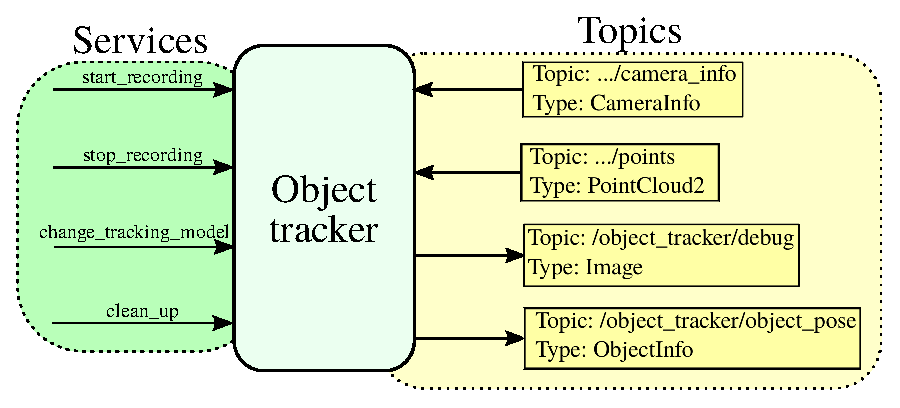
\includegraphics[width=0.85\textwidth]{images/object_tracker.eps}
\caption{Topics and services of the module Object Tracker\label{fig:Object_tracker}}
\end{figure}

It should be stated that the way to identify an object is done transforming the point clouds to an image and then from this are extracted a kind of SIFT features which describe the object. Then, the depth information is used to reaffirm that is the right object.

\subsection{Inverse kinematic solvers}
\label{sec:inverse_kinematic}

For solving inverse kinematics problems there are two main approaches: (1) numerical solution and (2) analytical (closed forms) solutions. 

On one hand, \textit{KDL} (Kinematics and Dynamics Library)\citep{KDL} is a library for computing forward and inverse kinematic queries with numeric recursive solving. This library is included in the MoveIt packages and it is the default solver if another one is not specified. However, it might be very slow or trap in local maximums due to recursive nature of numerical solutions for solving IK problems. 

On the other hand, \textit{OpenRAVE} (Open Robotics Automation Virtual Environment)\cite{Diankov2010} is a software for simulating and deploying planning algorithm. It provides a tool called IKFast which can generate C++ code (independent of any library) representing the model of the manipulator for solving forward and inverse kinematic queries. The generated code is able  to solve the request on the order of 4 microseconds \cite{Diankov}. In order to generate the C++ code for the robot, it should be provided a Collada model \cite{KhronosGroup} of the robot. Besides, as stated in Section \ref{sec:romeo_hardware}, the arms have one redundancy so for the C++ code generation is needed to specify which should be the free joint. Therefore, to solve IK queries with IKFast some of the key issues is to find proper values for this free joint and which joint should be selected. 


\chapter{Design of Romeo grasper package}
\label{cha:design}

The next stage introduces the general idea of the package here exposed. After this chapter, on the Implementation Chapter \ref{ch:implementation}, the package is explained in detail. 

Before the overview of the package, it should be stated that the purpose of \texttt{romeo\_grasper} is to combine the different dependencies to achieve grasping an object recognised by the camera. There are several dependencies, such as: (1) ROS packages which communicates with Romeo; (2) simulator and kinematic solvers to move the robot to the desired position; (3) ROS packages which generates the grasps; (4) camera drivers and (5) V4R software which allow to know where is the object respect to the camera.

A brief overview of this package can be understood by the Figure \ref{fig:overview_design}. First of all, the position of the object is got with the camera and V4R software. Then is time to compute a pre-grasping trajectory and a picking trajectory using inverse kinematics. The next stage is using the simulation to test these trajectories. After that, we send the joint commands to NAOqi through the Romeo ROS packages to finally move the robot joints and make the grasp.


\begin{figure}[h]
\centering
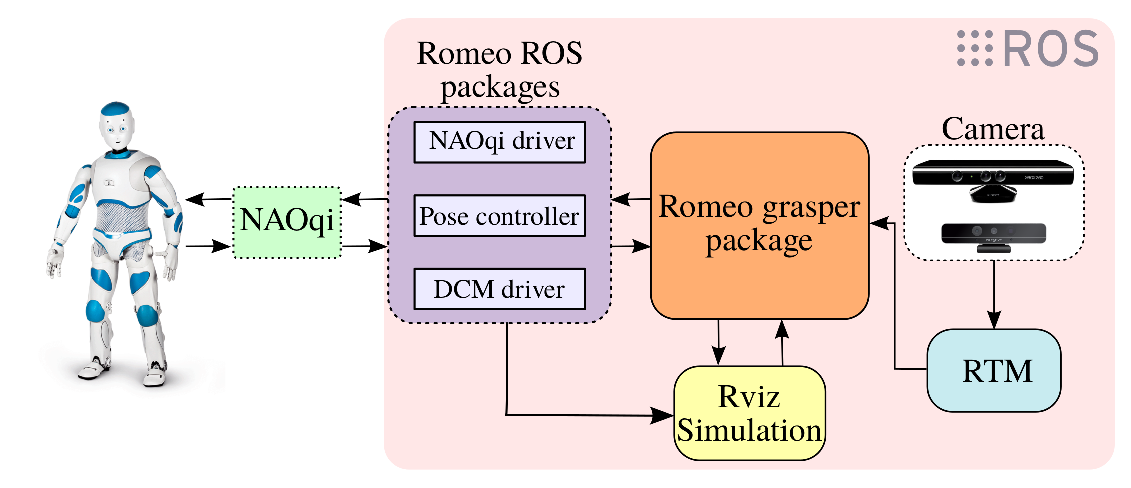
\includegraphics[width=0.85\textwidth]{images/package_design.eps}
\caption{Overview of the \texttt{Romeo grasper} package \label{fig:overview_design}}
\end{figure}

\section{Get position of the object}

In order to be able of grasping object which has been recognized by the camera, we need the position of the object on the robot reference. This position is got by the camera which should be positioned too. The ideal case would be using the Romeo RGB-D camera mentioned in Section \ref{sec:romeo_hardware}, because the relative position of the camera from the robot is known by the \texttt{romeo\_description} package and we don't need extra connections. But is not possible to get a good performance with it because, as mentioned in Section \ref{sec:romeo_ros}, the images of Romeo depth camera are useless. Moreover, the robot is not able to see its own arms till they are too far to work with because of the range of the camera. Seeing that we need to use an external camera to get the environment information.

Although, we can use any camera that can publish \texttt{PointClouds}, explained in Section \ref{sec:V4R}, is better to use the same type of camera used for the modeling of the object. In that case, we obtain a better performance of the V4R software and so less error for the global system. Once we have the camera, we can start positioning the camera.

\vspace{-10pt}
\subsection{Positioning the camera}
\label{sec:positioning_camera}

In \texttt{Romeo grasper} package there are different ways to make known to the robot the position of the camera:
\begin{enumerate}
\item Use of pre-known position of the camera relative to any link of the robot.
\item Use a reference object that the camera recognises and associates with a link of the robot.
\end{enumerate}

The first one, use the position of the link and then add the relative position to have the camera position on the robot reference and optionally can be set the RPY transformation for the camera. The second one uses the camera recognition software to know the position of the reference object. This object is associated with a link of the robot, so the position of the reference object is the position of the link. The ideal case would be that the reference object was itself the link robot. This case has been tested but without succeed because of the lack of \texttt{SIFT} points on the robot link surface, that makes difficult for the V4R software to detect the link. Because of that we use a reference object with an offset parameter to fix the error in the position, this offset parameter is explained in the following chapter, Section \ref{sec:model_object}.

Once we have the position of the camera, this is published to ROS. So it can be used for the simulator and to get the position of the object relative to the robot.

\vspace{-10pt}
\subsection{Calculate the object position}
\label{sec:design_object_position}

After having the position of the camera, we can start with the process of getting the position of the object. When the V4R software gives us the position, that is presented in camera coordinates. So we need to transform from this reference to robot reference. The way to do that is represented in the equation \eqref{eq:pos_robot_object}, so using the transform from camera reference to robot, got with the position and orientation of the camera on robot reference, and with the position on the camera reference results in the position on robot reference.

\begin{equation}
P_{robot}^{object} = T_{robot}^{camera} \cdot P_{camera}^{object} \label{eq:pos_robot_object}
\end{equation}


\section{Move the hand to object position}
\label{sec:design_move_hand}

Once we have the position of the object on the robot reference, we need first to move the hand to a pre-grasping position to then do the picking. In order to be able of this is required an inverse kinematic solver, like the two explained in Section \ref{sec:inverse_kinematic}, with this we get the joint trajectory which will be followed by the arm. Although, before move it, we should see in the simulator if there is any collision or not with external objects (collisions with the robot itself is checked automatically). Because of checking this and seeing the arm trajectory, after planning, by default, the package waits  the answer of the user with a service call, where you can choose: (1) to move the robot with this plan; (2) make another plan or (3) abort and wait till have another position. If we want to execute automatically the planned trajectory it only needs to put the ROS parameter \texttt{automatic\_execution} to \texttt{true}. Finally, after executing the plan for the pregrasp, it starts again the function but in this case to do the picking. As explained in Section \ref{sec:romeo_moveit_actions}, after testing different pickings, if someone is right it will be execute.

It should be stated that as said in Section \ref{sec:moveit_simple_grasps}, the left arm is configured to make a side grasp and the right arm for a top grasp. However, we can decide which arm use like others wide variety of parameters, as explained below. 

\section{Configuration and launching}
\label{sec:design_config}

Firstly, describe every parameter loaded to ROS with the file \texttt{romeo\_grasper.yaml}. Some of the concepts are explained in detail in the following Chapter \ref{ch:implementation}% So the description with the current default value is shown in the following table:
%TODO
%Revisar si la taula esta ben organitzada
\begin{table}[!h]
\begin{center}
\begin{tabulary}{\textwidth}{|l|c|J|}
\hline
\textbf{Parameter name} & \textbf{Default value} & \textbf{Description} \\ \hline
\texttt{move\_group} & left\_arm & Defines which is the group of links and joints controlled, see Table \ref{tab:tree_group_links_joint} in Section \ref{sec:romeo_hardware}.\\ \hline
\texttt{models\_directory} & \dots/data/models & Directory containing the modeled objects and their config files, see Section \ref{sec:model_object}\\  \hline
\texttt{model\_object\_name} & tea\_box & Name of the modeled object which should be grasped.\\  \hline
\texttt{model\_reference\_name} & ref\_tea\_box & Name of the modeled object which is used to position the reference link, explained in Section \ref{sec:visual-recognition}\\  \hline
\texttt{pose\_threshold} & 0.05 & Minimum position difference, from the old position to the current one, needed to consider that the position has changed.\\ \hline
\texttt{confidence\_threshold} & 0.25 & Minimum tracker confidence to use a position. If the position does not pass the threshold the position is rejected.\\ \hline
\texttt{ref\_confidence\_threshold} & 0.35 & Minimum tracker confidence to use a position to set the reference link.\\ \hline
\texttt{reachVsGrasp} & true & Boolean to set the way to do the planning of the pre-grasp, using \texttt{reachAction} or \texttt{graspPlan}. More information in Sections \ref{sec:romeo_moveit_actions} and \ref{sec:planning_pregrasp}\\ \hline
\texttt{max\_velocity\_scaling\_factor} & 0.1 & Maximum factor of speed for the joints.\\ \hline
\texttt{tolerance\_step} & 0.1 & Step which increments the goal tolerance for every attempt in \texttt{reachAction} and \texttt{pickAction} function.\\ \hline
\texttt{tolerance\_min} & 0.1 & Initial goal tolerance for planning and picking.\\ \hline
\texttt{planning\_time} & 20 & Maximum planning time for each attempt.\\ \hline
\texttt{attempts\_max} & 3 & Maximum number of attempts.\\ \hline
\multicolumn{3}{|r|}{\small\sl continued on next page}\\
\hline
\end{tabulary}
\end{center}
\end{table}

\break

\begin{table}[!h]
\begin{center}
\begin{tabulary}{\textwidth}{|l|c|J|}
\hline
\multicolumn{3}{|l|}{\small\sl continued from previous page}\\ \hline
\textbf{Parameter name} & \textbf{Default value} & \textbf{Description} \\ \hline
\texttt{base\_link\_frame\_id} & base\_link & Base frame of the robot.\\ \hline
\texttt{camera\_in\_front} & false & Boolean to know if the camera is in front of the robot or next to it. More information in Section \ref{sec:impl_camera_approach}\\ \hline
\texttt{camera\_ref\_frame\_id} & l\_wrist & Frame of the link used as reference, see Section \ref{sec:visual-recognition}. \\ \hline
\texttt{camera\_link} & camera\_link & Frame used to set the position of the camera.\\ \hline
\texttt{object\_frame\_id} & object\_frame & Frame of the object that should be grasped.\\ \hline
\multirow{1}{*}{\texttt{camera\_pose\_x}} & \multirow{1}{*}{-0.11} & \multirow{3}{\hsize}{Coords of the camera when camera position is pre-known, more in Section \ref{sec:pre-known_distance}} \\ \cline{1-2}
\multirow{1}{*}{\texttt{camera\_pose\_y}} & \multirow{1}{*}{0.62} & \\ \cline{1-2}
\multirow{1}{*}{\texttt{camera\_pose\_z}} & \multirow{1}{*}{0.14} & \\ \hline
\multirow{1}{*}{\texttt{camera\_pose\_roll}} & \multirow{1}{*}{$\frac{\pi}{18}$} & \multirow{3}{\hsize}{Orientation of the camera in RPY when camera position is pre-known, see Section \ref{sec:pre-known_distance}} \\ \cline{1-2}
\multirow{1}{*}{\texttt{camera\_pose\_pitch}} & \multirow{1}{*}{0} & \\ \cline{1-2}
\multirow{1}{*}{\texttt{camera\_pose\_yaw}} & \multirow{1}{*}{$-\frac{\pi}{2}$} & \\ \hline
\texttt{camera\_frame\_id} & camera\_rgb\_optical\_frame & Frame of the camera following the ROS Enhancement Proposals (REPs) as an optical camera frame \cite{Foote}.\\ \hline
\end{tabulary}
\caption{Description and default value of every parameter of \texttt{romeo\_grasper.yaml}\label{tab:param_romeo_grasper}}
%\multicolumn{3}{|r|}{\small\sl continued on next page}\\
%\hline
\end{center}
\end{table}

%\break
%
%\begin{table}[!h]
%\begin{center}
%\begin{tabulary}{\textwidth}{|l|c|J|}
%\hline
%\multicolumn{3}{|l|}{\small\sl continued from previous page}\\ \hline
%\textbf{Parameter name} & \textbf{Default value} & \textbf{Description} \\ \hline
%
%\end{center}
%\end{table}

Referring to the launching, in \texttt{romeo\_grasper} package, there is a main launch file which is named as \texttt{romeo\_grasper.launch}. This run the main node of the package loading the following parameter files:

\begin{itemize}
\item \texttt{romeo\_grasper.yaml}: the one explained above.
\item \texttt{kinematics.yaml} from \texttt{romeo\_moveit\_config} package: which contain the features about the kinematic solver.
\item \texttt{romeo\_grasper\_data.yaml} from \texttt{moveit\_simple\_grasps}: file with the geometry of the romeo gripper. 
\item \texttt{model\_config.yaml} for every modeled object used: configuration file of the modeled object. This file should be in the following namespace: \texttt{models/MODEL\_NAME}.
\end{itemize}

Moreover, the launcher has the following arguments which are loaded as parameters for the node and these define how the package should work.

\begin{table}[!h]
\begin{center}
\begin{tabulary}{0.9\textwidth}{|l|c|J|}
\hline
\textbf{Parameter name} & \textbf{Default value} & \textbf{Description} \\ \hline
\texttt{launch\_full} & false & In case of launch all the nodes together \texttt{romeo\_grasper} waits some seconds to give time to the other nodes to be ready.\\ \hline
\texttt{verbose} & false & Enables verbose mode.\\ \hline
\texttt{debug} & false & Enables debug mode.\\ \hline
\texttt{tracking} & true & Should be enable when a real camera is used.\\ \hline
\texttt{pose\_camera\_preknown} & false & Enable use of the parameters \texttt{camera\_pose\_x/y/z} to set camera position.\\ \hline
\texttt{simulation} & false & Used when is not working with real Romeo\\ \hline
\texttt{automatic\_execution} & false & Avoid waiting for user answer to execute the plan\\ \hline
\end{tabulary}
\caption{Description and default value of \texttt{romeo\_grasper.launch} arguments.\label{tab:arg_launch_romeo_grasper}}
\end{center}
\end{table}

Although, a real camera were not used, so being \texttt{tracking} false, the position of the object can be given to \texttt{romeo\_grasper} though the \texttt{object\_tracker/object\_pose} topic as is done by the V4R software.

However, the previously launcher cannot be run alone, it needs other nodes to work properly. Therefore, there are two more launchers which run these nodes automatically: 
\begin{itemize}
\item \texttt{romeo\_grasper\_full.launch} to run on the real robot.
\item \texttt{romeo\_grasper\_demo\_full.launch} to run on a simulation or on the real robot but without moving it.
\end{itemize}

Both launchers run \texttt{romeo\_grasper.launch}, the \texttt{romeo\_full\_py.launch} launcher which is the one for \texttt{naoqi\_driver\_py} and \texttt{romeo\_sensor\_py} packages and an Rviz launcher. However, the last one for the demo launch is run with \texttt{fake\_execution}, so it doesn't move the robot. Furthermore, they need a way to move the robot, when is with the real robot is though \texttt{DCM} package and with the simulation is though \texttt{naoqi\_pose} package. Therefore, the real launcher runs the \texttt{DCM} driver and the demo launcher runs the \texttt{pose\_controller} node. For more information about these last packages and nodes see Section \ref{sec:romeo_ros}.

It needs to be stated that to use a real camera is necessary to launch another node. There are two possible cases: (1) use a RealSense camera or (2) use a camera through openNi.\footnote{Installation of the camera drivers explained in Appendix \ref{app:camera_instal}.} On one hand, the RealSense camera can be launch with the \texttt{use\_realsense} argument in the launchers. On the other hand, for the openNi case, should be run the following command on a new terminal:

\begin{lstlisting}[language=ROS]
roslaunch openni_launch openni.launch depth_registration:=true
\end{lstlisting}

Finally, it should be mentioned that the Rviz configuration and launching files are copied from \texttt{romeo\_moveit\_config}, but modified to have a more adapted features for this package. 


\chapter{Implementation}
\label{ch:implementation}

At this stage the details of every process are explained. So the parts briefly exposed previously are analysed deeply. Sometimes are used knowledge described in previous chapters, but they have the corresponding reference to make easier the reading.

\section{Model Object class}
\label{sec:model_object}

This class represent, in the \texttt{Romeo grasper} package, an object that has been previously modeled with the V4R Toolbox. This class allow to create, remove and update every object independently in the simulator and to calculate its own position with the pertinent correction on the robot reference, given the position on camera reference. 

At the initialization of this class, it should be associated with one of the modeled object with the pertinent configuration file \texttt{model\_config.yaml} in the same folder of the modeled object.\footnote{In the package the folder for every model is placed at \texttt{data/models/MODEL\_NAME}.} The config file has the following parameters:

\begin{itemize}
\item \textbf{offset\_x$/$y$/$z}: the origin established by the V4R Toolbox may be is not the desired one for the grasp. This offset use the orientation provided by V4R Toolbox.
\item \textbf{shapeType}: shape used in the simulator. For now only supports \texttt{cylinder}.
\item \textbf{size}: set the radius of the cylinder.
\item \textbf{size\_l}: set the longitude of the cylinder.
\end{itemize}

\newpage
Every modeled object that wants to be used must have the configuration file loaded in the launch file. So the following line should be used for every model in the node namespace \textit{MODEL\_NAME} for the name of the model.
\begin{lstlisting}[language=ROS]
<rosparam command="load" ns="models/MODEL_NAME" file="$(find romeo_grasper)/data/models/MODEL_NAME/model_config.yaml" />
\end{lstlisting}

An overview of the processes done by this class is showed below, on Figure \ref{fig:flow_model_object}. Moreover, the last part of the flow sequence is explained in detail on Figure \ref{fig:model_object_transform}.

\begin{figure}[h]
\centering
% Graphic for TeX using PGF
% Title: /home/lluis/Escritorio/TFM/Informe/images/model_object_diagram.dia
% Creator: Dia v0.97.2
% CreationDate: Thu May 19 11:39:34 2016
% For: lluis
% \usepackage{tikz}
% The following commands are not supported in PSTricks at present
% We define them conditionally, so when they are implemented,
% this pgf file will use them.
\ifx\du\undefined
  \newlength{\du}
\fi
\setlength{\du}{15\unitlength}
\begin{tikzpicture}
\pgftransformxscale{1.000000}
\pgftransformyscale{-1.000000}
\definecolor{dialinecolor}{rgb}{0.000000, 0.000000, 0.000000}
\pgfsetstrokecolor{dialinecolor}
\definecolor{dialinecolor}{rgb}{1.000000, 1.000000, 1.000000}
\pgfsetfillcolor{dialinecolor}
\definecolor{dialinecolor}{rgb}{0.678431, 0.847059, 0.901961}
\pgfsetfillcolor{dialinecolor}
\fill (12.205200\du,4.120720\du)--(12.205200\du,6.820720\du)--(19.405200\du,6.820720\du)--(19.405200\du,4.120720\du)--cycle;
\pgfsetlinewidth{0.100000\du}
\pgfsetdash{}{0pt}
\pgfsetdash{}{0pt}
\pgfsetmiterjoin
\definecolor{dialinecolor}{rgb}{0.000000, 0.000000, 0.000000}
\pgfsetstrokecolor{dialinecolor}
\draw (12.205200\du,4.120720\du)--(12.205200\du,6.820720\du)--(19.405200\du,6.820720\du)--(19.405200\du,4.120720\du)--cycle;
% setfont left to latex
\definecolor{dialinecolor}{rgb}{0.000000, 0.000000, 0.000000}
\pgfsetstrokecolor{dialinecolor}
\node at (15.805200\du,5.265720\du){Model Object Class};
% setfont left to latex
\definecolor{dialinecolor}{rgb}{0.000000, 0.000000, 0.000000}
\pgfsetstrokecolor{dialinecolor}
\node at (15.805200\du,6.065720\du){Creation};
\definecolor{dialinecolor}{rgb}{0.678431, 0.847059, 0.901961}
\pgfsetfillcolor{dialinecolor}
\fill (11.242800\du,7.957890\du)--(11.242800\du,10.657890\du)--(20.337800\du,10.657890\du)--(20.337800\du,7.957890\du)--cycle;
\pgfsetlinewidth{0.100000\du}
\pgfsetdash{}{0pt}
\pgfsetdash{}{0pt}
\pgfsetmiterjoin
\definecolor{dialinecolor}{rgb}{0.000000, 0.000000, 0.000000}
\pgfsetstrokecolor{dialinecolor}
\draw (11.242800\du,7.957890\du)--(11.242800\du,10.657890\du)--(20.337800\du,10.657890\du)--(20.337800\du,7.957890\du)--cycle;
% setfont left to latex
\definecolor{dialinecolor}{rgb}{0.000000, 0.000000, 0.000000}
\pgfsetstrokecolor{dialinecolor}
\node at (15.790300\du,9.102890\du){Load object and};
% setfont left to latex
\definecolor{dialinecolor}{rgb}{0.000000, 0.000000, 0.000000}
\pgfsetstrokecolor{dialinecolor}
\node at (15.790300\du,9.902890\du){enviornment parameters};
\pgfsetlinewidth{0.100000\du}
\pgfsetdash{}{0pt}
\pgfsetdash{}{0pt}
\pgfsetbuttcap
\pgfsetmiterjoin
\pgfsetlinewidth{0.100000\du}
\pgfsetbuttcap
\pgfsetmiterjoin
\pgfsetdash{}{0pt}
\definecolor{dialinecolor}{rgb}{1.000000, 0.878431, 0.650980}
\pgfsetfillcolor{dialinecolor}
\pgfpathmoveto{\pgfpoint{10.754810\du}{11.645500\du}}
\pgfpathlineto{\pgfpoint{20.857310\du}{11.645500\du}}
\pgfpathlineto{\pgfpoint{22.877810\du}{12.314734\du}}
\pgfpathlineto{\pgfpoint{20.857310\du}{12.983968\du}}
\pgfpathlineto{\pgfpoint{10.754810\du}{12.983968\du}}
\pgfpathlineto{\pgfpoint{8.734310\du}{12.314734\du}}
\pgfpathlineto{\pgfpoint{10.754810\du}{11.645500\du}}
\pgfusepath{fill}
\definecolor{dialinecolor}{rgb}{0.000000, 0.000000, 0.000000}
\pgfsetstrokecolor{dialinecolor}
\pgfpathmoveto{\pgfpoint{10.754810\du}{11.645500\du}}
\pgfpathlineto{\pgfpoint{20.857310\du}{11.645500\du}}
\pgfpathlineto{\pgfpoint{22.877810\du}{12.314734\du}}
\pgfpathlineto{\pgfpoint{20.857310\du}{12.983968\du}}
\pgfpathlineto{\pgfpoint{10.754810\du}{12.983968\du}}
\pgfpathlineto{\pgfpoint{8.734310\du}{12.314734\du}}
\pgfpathlineto{\pgfpoint{10.754810\du}{11.645500\du}}
\pgfusepath{stroke}
% setfont left to latex
\definecolor{dialinecolor}{rgb}{0.000000, 0.000000, 0.000000}
\pgfsetstrokecolor{dialinecolor}
\node at (15.806060\du,12.514734\du){Wait till first data from camera};
\definecolor{dialinecolor}{rgb}{0.678431, 0.847059, 0.901961}
\pgfsetfillcolor{dialinecolor}
\fill (11.142100\du,15.311400\du)--(11.142100\du,18.811400\du)--(20.467100\du,18.811400\du)--(20.467100\du,15.311400\du)--cycle;
\pgfsetlinewidth{0.100000\du}
\pgfsetdash{}{0pt}
\pgfsetdash{}{0pt}
\pgfsetmiterjoin
\definecolor{dialinecolor}{rgb}{0.000000, 0.000000, 0.000000}
\pgfsetstrokecolor{dialinecolor}
\draw (11.142100\du,15.311400\du)--(11.142100\du,18.811400\du)--(20.467100\du,18.811400\du)--(20.467100\du,15.311400\du)--cycle;
% setfont left to latex
\definecolor{dialinecolor}{rgb}{0.000000, 0.000000, 0.000000}
\pgfsetstrokecolor{dialinecolor}
\node at (15.804600\du,16.456400\du){Transform pose with};
% setfont left to latex
\definecolor{dialinecolor}{rgb}{0.000000, 0.000000, 0.000000}
\pgfsetstrokecolor{dialinecolor}
\node at (15.804600\du,17.256400\du){offset from camera};
% setfont left to latex
\definecolor{dialinecolor}{rgb}{0.000000, 0.000000, 0.000000}
\pgfsetstrokecolor{dialinecolor}
\node at (15.804600\du,18.056400\du){ frame to base\_link frame};
\pgfsetlinewidth{0.100000\du}
\pgfsetdash{}{0pt}
\pgfsetdash{}{0pt}
\pgfsetmiterjoin
\pgfsetbuttcap
{
\definecolor{dialinecolor}{rgb}{0.000000, 0.000000, 0.000000}
\pgfsetfillcolor{dialinecolor}
% was here!!!
\pgfsetarrowsend{stealth}
{\pgfsetcornersarced{\pgfpoint{0.000000\du}{0.000000\du}}\definecolor{dialinecolor}{rgb}{0.000000, 0.000000, 0.000000}
\pgfsetstrokecolor{dialinecolor}
\draw (18.064100\du,10.657900\du)--(18.064100\du,11.218100\du)--(24.871345\du,11.218100\du)--(24.871345\du,13.438275\du);
}}
\definecolor{dialinecolor}{rgb}{0.678431, 0.847059, 0.901961}
\pgfsetfillcolor{dialinecolor}
\fill (12.434900\du,19.868500\du)--(12.434900\du,21.768500\du)--(19.164900\du,21.768500\du)--(19.164900\du,19.868500\du)--cycle;
\pgfsetlinewidth{0.100000\du}
\pgfsetdash{}{0pt}
\pgfsetdash{}{0pt}
\pgfsetmiterjoin
\definecolor{dialinecolor}{rgb}{0.000000, 0.000000, 0.000000}
\pgfsetstrokecolor{dialinecolor}
\draw (12.434900\du,19.868500\du)--(12.434900\du,21.768500\du)--(19.164900\du,21.768500\du)--(19.164900\du,19.868500\du)--cycle;
% setfont left to latex
\definecolor{dialinecolor}{rgb}{0.000000, 0.000000, 0.000000}
\pgfsetstrokecolor{dialinecolor}
\node at (15.799900\du,21.013500\du){Update final pose};
\definecolor{dialinecolor}{rgb}{0.631373, 0.862745, 0.631373}
\pgfsetfillcolor{dialinecolor}
\fill (20.938445\du,16.826200\du)--(20.938445\du,21.126200\du)--(28.805945\du,21.126200\du)--(28.805945\du,16.826200\du)--cycle;
\pgfsetlinewidth{0.100000\du}
\pgfsetdash{}{0pt}
\pgfsetdash{}{0pt}
\pgfsetmiterjoin
\definecolor{dialinecolor}{rgb}{0.000000, 0.000000, 0.000000}
\pgfsetstrokecolor{dialinecolor}
\draw (20.938445\du,16.826200\du)--(20.938445\du,21.126200\du)--(28.805945\du,21.126200\du)--(28.805945\du,16.826200\du)--cycle;
% setfont left to latex
\definecolor{dialinecolor}{rgb}{0.000000, 0.000000, 0.000000}
\pgfsetstrokecolor{dialinecolor}
\node at (24.872195\du,17.971200\du){Publish transform };
% setfont left to latex
\definecolor{dialinecolor}{rgb}{0.000000, 0.000000, 0.000000}
\pgfsetstrokecolor{dialinecolor}
\node at (24.872195\du,18.771200\du){from base\_link frame};
% setfont left to latex
\definecolor{dialinecolor}{rgb}{0.000000, 0.000000, 0.000000}
\pgfsetstrokecolor{dialinecolor}
\node at (24.872195\du,19.571200\du){to object frame};
% setfont left to latex
\definecolor{dialinecolor}{rgb}{0.000000, 0.000000, 0.000000}
\pgfsetstrokecolor{dialinecolor}
\node at (24.872195\du,20.371200\du){every 100 ms};
\pgfsetlinewidth{0.100000\du}
\pgfsetdash{}{0pt}
\pgfsetdash{}{0pt}
\pgfsetbuttcap
{
\definecolor{dialinecolor}{rgb}{0.000000, 0.000000, 0.000000}
\pgfsetfillcolor{dialinecolor}
% was here!!!
\pgfsetarrowsend{stealth}
\definecolor{dialinecolor}{rgb}{0.000000, 0.000000, 0.000000}
\pgfsetstrokecolor{dialinecolor}
\draw (15.804600\du,18.811400\du)--(15.799900\du,19.868500\du);
}
\pgfsetlinewidth{0.100000\du}
\pgfsetdash{}{0pt}
\pgfsetdash{}{0pt}
\pgfsetbuttcap
{
\definecolor{dialinecolor}{rgb}{0.000000, 0.000000, 0.000000}
\pgfsetfillcolor{dialinecolor}
% was here!!!
\pgfsetarrowsend{stealth}
\definecolor{dialinecolor}{rgb}{0.000000, 0.000000, 0.000000}
\pgfsetstrokecolor{dialinecolor}
\draw (24.871345\du,14.863417\du)--(24.872195\du,16.826200\du);
}
\pgfsetlinewidth{0.100000\du}
\pgfsetdash{}{0pt}
\pgfsetdash{}{0pt}
\pgfsetbuttcap
\pgfsetmiterjoin
\pgfsetlinewidth{0.100000\du}
\pgfsetbuttcap
\pgfsetmiterjoin
\pgfsetdash{}{0pt}
\definecolor{dialinecolor}{rgb}{1.000000, 0.878431, 0.650980}
\pgfsetfillcolor{dialinecolor}
\pgfpathmoveto{\pgfpoint{19.801345\du}{13.438275\du}}
\pgfpathlineto{\pgfpoint{29.941345\du}{13.438275\du}}
\pgfpathlineto{\pgfpoint{31.969345\du}{14.150846\du}}
\pgfpathlineto{\pgfpoint{29.941345\du}{14.863417\du}}
\pgfpathlineto{\pgfpoint{19.801345\du}{14.863417\du}}
\pgfpathlineto{\pgfpoint{17.773345\du}{14.150846\du}}
\pgfpathlineto{\pgfpoint{19.801345\du}{13.438275\du}}
\pgfusepath{fill}
\definecolor{dialinecolor}{rgb}{0.000000, 0.000000, 0.000000}
\pgfsetstrokecolor{dialinecolor}
\pgfpathmoveto{\pgfpoint{19.801345\du}{13.438275\du}}
\pgfpathlineto{\pgfpoint{29.941345\du}{13.438275\du}}
\pgfpathlineto{\pgfpoint{31.969345\du}{14.150846\du}}
\pgfpathlineto{\pgfpoint{29.941345\du}{14.863417\du}}
\pgfpathlineto{\pgfpoint{19.801345\du}{14.863417\du}}
\pgfpathlineto{\pgfpoint{17.773345\du}{14.150846\du}}
\pgfpathlineto{\pgfpoint{19.801345\du}{13.438275\du}}
\pgfusepath{stroke}
% setfont left to latex
\definecolor{dialinecolor}{rgb}{0.000000, 0.000000, 0.000000}
\pgfsetstrokecolor{dialinecolor}
\node at (24.871345\du,14.350846\du){Wait till first pose update done};
\pgfsetlinewidth{0.100000\du}
\pgfsetdash{}{0pt}
\pgfsetdash{}{0pt}
\pgfsetbuttcap
\pgfsetmiterjoin
\pgfsetlinewidth{0.100000\du}
\pgfsetbuttcap
\pgfsetmiterjoin
\pgfsetdash{}{0pt}
\definecolor{dialinecolor}{rgb}{1.000000, 0.878431, 0.650980}
\pgfsetfillcolor{dialinecolor}
\pgfpathmoveto{\pgfpoint{2.566605\du}{13.443649\du}}
\pgfpathlineto{\pgfpoint{11.759105\du}{13.443649\du}}
\pgfpathlineto{\pgfpoint{13.597605\du}{14.147320\du}}
\pgfpathlineto{\pgfpoint{11.759105\du}{14.850991\du}}
\pgfpathlineto{\pgfpoint{2.566605\du}{14.850991\du}}
\pgfpathlineto{\pgfpoint{0.728105\du}{14.147320\du}}
\pgfpathlineto{\pgfpoint{2.566605\du}{13.443649\du}}
\pgfusepath{fill}
\definecolor{dialinecolor}{rgb}{0.000000, 0.000000, 0.000000}
\pgfsetstrokecolor{dialinecolor}
\pgfpathmoveto{\pgfpoint{2.566605\du}{13.443649\du}}
\pgfpathlineto{\pgfpoint{11.759105\du}{13.443649\du}}
\pgfpathlineto{\pgfpoint{13.597605\du}{14.147320\du}}
\pgfpathlineto{\pgfpoint{11.759105\du}{14.850991\du}}
\pgfpathlineto{\pgfpoint{2.566605\du}{14.850991\du}}
\pgfpathlineto{\pgfpoint{0.728105\du}{14.147320\du}}
\pgfpathlineto{\pgfpoint{2.566605\du}{13.443649\du}}
\pgfusepath{stroke}
% setfont left to latex
\definecolor{dialinecolor}{rgb}{0.000000, 0.000000, 0.000000}
\pgfsetstrokecolor{dialinecolor}
\node at (7.162855\du,14.347320\du){Wait new data from camera};
\pgfsetlinewidth{0.100000\du}
\pgfsetdash{}{0pt}
\pgfsetdash{}{0pt}
\pgfsetmiterjoin
\pgfsetbuttcap
{
\definecolor{dialinecolor}{rgb}{0.000000, 0.000000, 0.000000}
\pgfsetfillcolor{dialinecolor}
% was here!!!
\pgfsetarrowsend{stealth}
{\pgfsetcornersarced{\pgfpoint{0.000000\du}{0.000000\du}}\definecolor{dialinecolor}{rgb}{0.000000, 0.000000, 0.000000}
\pgfsetstrokecolor{dialinecolor}
\draw (15.799900\du,21.768500\du)--(15.799900\du,22.233800\du)--(0.532559\du,22.233800\du)--(0.532559\du,12.405408\du)--(7.162855\du,12.405408\du)--(7.162855\du,13.443649\du);
}}
\pgfsetlinewidth{0.100000\du}
\pgfsetdash{}{0pt}
\pgfsetdash{}{0pt}
\pgfsetmiterjoin
\pgfsetbuttcap
{
\definecolor{dialinecolor}{rgb}{0.000000, 0.000000, 0.000000}
\pgfsetfillcolor{dialinecolor}
% was here!!!
\pgfsetarrowsend{stealth}
{\pgfsetcornersarced{\pgfpoint{0.000000\du}{0.000000\du}}\definecolor{dialinecolor}{rgb}{0.000000, 0.000000, 0.000000}
\pgfsetstrokecolor{dialinecolor}
\draw (7.162855\du,14.850991\du)--(7.162855\du,17.061400\du)--(11.142100\du,17.061400\du);
}}
\pgfsetlinewidth{0.100000\du}
\pgfsetdash{}{0pt}
\pgfsetdash{}{0pt}
\pgfsetbuttcap
{
\definecolor{dialinecolor}{rgb}{0.000000, 0.000000, 0.000000}
\pgfsetfillcolor{dialinecolor}
% was here!!!
\pgfsetarrowsend{stealth}
\definecolor{dialinecolor}{rgb}{0.000000, 0.000000, 0.000000}
\pgfsetstrokecolor{dialinecolor}
\draw (15.806100\du,12.983900\du)--(15.804600\du,15.311400\du);
}
\pgfsetlinewidth{0.100000\du}
\pgfsetdash{}{0pt}
\pgfsetdash{}{0pt}
\pgfsetbuttcap
{
\definecolor{dialinecolor}{rgb}{0.000000, 0.000000, 0.000000}
\pgfsetfillcolor{dialinecolor}
% was here!!!
\pgfsetarrowsend{stealth}
\definecolor{dialinecolor}{rgb}{0.000000, 0.000000, 0.000000}
\pgfsetstrokecolor{dialinecolor}
\draw (15.799762\du,10.707831\du)--(15.806100\du,11.645500\du);
}
\pgfsetlinewidth{0.100000\du}
\pgfsetdash{}{0pt}
\pgfsetdash{}{0pt}
\pgfsetbuttcap
{
\definecolor{dialinecolor}{rgb}{0.000000, 0.000000, 0.000000}
\pgfsetfillcolor{dialinecolor}
% was here!!!
\pgfsetarrowsend{stealth}
\definecolor{dialinecolor}{rgb}{0.000000, 0.000000, 0.000000}
\pgfsetstrokecolor{dialinecolor}
\draw (15.805200\du,6.820720\du)--(15.790300\du,7.957890\du);
}
\pgfsetlinewidth{0.100000\du}
\pgfsetdash{}{0pt}
\pgfsetdash{}{0pt}
\pgfsetbuttcap
\pgfsetmiterjoin
\pgfsetlinewidth{0.100000\du}
\pgfsetbuttcap
\pgfsetmiterjoin
\pgfsetdash{}{0pt}
\definecolor{dialinecolor}{rgb}{0.000000, 0.000000, 0.000000}
\pgfsetstrokecolor{dialinecolor}
\draw (22.396300\du,8.741380\du)--(22.396300\du,9.899275\du);
\pgfsetbuttcap
\pgfsetmiterjoin
\pgfsetdash{}{0pt}
\definecolor{dialinecolor}{rgb}{0.000000, 0.000000, 0.000000}
\pgfsetstrokecolor{dialinecolor}
\draw (22.396300\du,8.741380\du)--(28.284830\du,8.741380\du);
\pgfsetbuttcap
\pgfsetmiterjoin
\pgfsetdash{}{0pt}
\definecolor{dialinecolor}{rgb}{0.000000, 0.000000, 0.000000}
\pgfsetstrokecolor{dialinecolor}
\draw (22.396300\du,9.899275\du)--(28.284830\du,9.899275\du);
% setfont left to latex
\definecolor{dialinecolor}{rgb}{0.000000, 0.000000, 0.000000}
\pgfsetstrokecolor{dialinecolor}
\node at (25.487778\du,9.549275\du){};
% setfont left to latex
\definecolor{dialinecolor}{rgb}{0.000000, 0.000000, 0.000000}
\pgfsetstrokecolor{dialinecolor}
\node[anchor=west] at (22.423900\du,9.302650\du){ROS Parameters};
\pgfsetlinewidth{0.100000\du}
\pgfsetdash{}{0pt}
\pgfsetdash{}{0pt}
\pgfsetbuttcap
{
\definecolor{dialinecolor}{rgb}{0.000000, 0.000000, 0.000000}
\pgfsetfillcolor{dialinecolor}
% was here!!!
\pgfsetarrowsend{stealth}
\definecolor{dialinecolor}{rgb}{0.000000, 0.000000, 0.000000}
\pgfsetstrokecolor{dialinecolor}
\draw (22.396300\du,9.320320\du)--(20.337800\du,9.307890\du);
}
\end{tikzpicture}

\caption{Flow sequence of ModelObject class\label{fig:flow_model_object}}
\end{figure}

\begin{figure}[h]
\centering
% Graphic for TeX using PGF
% Title: /home/lluis/Escritorio/TFM/Informe/images/model_object_transform.dia
% Creator: Dia v0.97.2
% CreationDate: Thu May 19 12:05:21 2016
% For: lluis
% \usepackage{tikz}
% The following commands are not supported in PSTricks at present
% We define them conditionally, so when they are implemented,
% this pgf file will use them.
\ifx\du\undefined
  \newlength{\du}
\fi
\setlength{\du}{15\unitlength}
\begin{tikzpicture}
\pgftransformxscale{1.000000}
\pgftransformyscale{-1.000000}
\definecolor{dialinecolor}{rgb}{0.000000, 0.000000, 0.000000}
\pgfsetstrokecolor{dialinecolor}
\definecolor{dialinecolor}{rgb}{1.000000, 1.000000, 1.000000}
\pgfsetfillcolor{dialinecolor}
\definecolor{dialinecolor}{rgb}{0.678431, 0.847059, 0.901961}
\pgfsetfillcolor{dialinecolor}
\fill (10.731784\du,6.400000\du)--(10.731784\du,8.300000\du)--(18.394284\du,8.300000\du)--(18.394284\du,6.400000\du)--cycle;
\pgfsetlinewidth{0.100000\du}
\pgfsetdash{}{0pt}
\pgfsetdash{}{0pt}
\pgfsetmiterjoin
\definecolor{dialinecolor}{rgb}{0.000000, 0.000000, 0.000000}
\pgfsetstrokecolor{dialinecolor}
\draw (10.731784\du,6.400000\du)--(10.731784\du,8.300000\du)--(18.394284\du,8.300000\du)--(18.394284\du,6.400000\du)--cycle;
% setfont left to latex
\definecolor{dialinecolor}{rgb}{0.000000, 0.000000, 0.000000}
\pgfsetstrokecolor{dialinecolor}
\node at (14.563034\du,7.545000\du){Start Transformation};
\definecolor{dialinecolor}{rgb}{0.678431, 0.847059, 0.901961}
\pgfsetfillcolor{dialinecolor}
\fill (9.967848\du,9.300000\du)--(9.967848\du,11.200000\du)--(19.255348\du,11.200000\du)--(19.255348\du,9.300000\du)--cycle;
\pgfsetlinewidth{0.100000\du}
\pgfsetdash{}{0pt}
\pgfsetdash{}{0pt}
\pgfsetmiterjoin
\definecolor{dialinecolor}{rgb}{0.000000, 0.000000, 0.000000}
\pgfsetstrokecolor{dialinecolor}
\draw (9.967848\du,9.300000\du)--(9.967848\du,11.200000\du)--(19.255348\du,11.200000\du)--(19.255348\du,9.300000\du)--cycle;
% setfont left to latex
\definecolor{dialinecolor}{rgb}{0.000000, 0.000000, 0.000000}
\pgfsetstrokecolor{dialinecolor}
\node at (14.611598\du,10.445000\du){Get position from camera};
\pgfsetlinewidth{0.100000\du}
\pgfsetdash{}{0pt}
\pgfsetdash{}{0pt}
\pgfsetbuttcap
\pgfsetmiterjoin
\pgfsetlinewidth{0.100000\du}
\pgfsetbuttcap
\pgfsetmiterjoin
\pgfsetdash{}{0pt}
\definecolor{dialinecolor}{rgb}{1.000000, 0.878431, 0.650980}
\pgfsetfillcolor{dialinecolor}
\pgfpathmoveto{\pgfpoint{8.423750\du}{12.587511\du}}
\pgfpathlineto{\pgfpoint{16.076250\du}{12.587511\du}}
\pgfpathlineto{\pgfpoint{17.606750\du}{13.937511\du}}
\pgfpathlineto{\pgfpoint{16.076250\du}{15.287511\du}}
\pgfpathlineto{\pgfpoint{8.423750\du}{15.287511\du}}
\pgfpathlineto{\pgfpoint{6.893250\du}{13.937511\du}}
\pgfpathlineto{\pgfpoint{8.423750\du}{12.587511\du}}
\pgfusepath{fill}
\definecolor{dialinecolor}{rgb}{0.000000, 0.000000, 0.000000}
\pgfsetstrokecolor{dialinecolor}
\pgfpathmoveto{\pgfpoint{8.423750\du}{12.587511\du}}
\pgfpathlineto{\pgfpoint{16.076250\du}{12.587511\du}}
\pgfpathlineto{\pgfpoint{17.606750\du}{13.937511\du}}
\pgfpathlineto{\pgfpoint{16.076250\du}{15.287511\du}}
\pgfpathlineto{\pgfpoint{8.423750\du}{15.287511\du}}
\pgfpathlineto{\pgfpoint{6.893250\du}{13.937511\du}}
\pgfpathlineto{\pgfpoint{8.423750\du}{12.587511\du}}
\pgfusepath{stroke}
% setfont left to latex
\definecolor{dialinecolor}{rgb}{0.000000, 0.000000, 0.000000}
\pgfsetstrokecolor{dialinecolor}
\node at (12.250000\du,13.337511\du){Wait till transformation};
% setfont left to latex
\definecolor{dialinecolor}{rgb}{0.000000, 0.000000, 0.000000}
\pgfsetstrokecolor{dialinecolor}
\node at (12.250000\du,14.137511\du){from camera to object};
% setfont left to latex
\definecolor{dialinecolor}{rgb}{0.000000, 0.000000, 0.000000}
\pgfsetstrokecolor{dialinecolor}
\node at (12.250000\du,14.937511\du){is published};
\definecolor{dialinecolor}{rgb}{0.678431, 0.847059, 0.901961}
\pgfsetfillcolor{dialinecolor}
\fill (19.161250\du,12.608845\du)--(19.161250\du,15.308845\du)--(25.938750\du,15.308845\du)--(25.938750\du,12.608845\du)--cycle;
\pgfsetlinewidth{0.100000\du}
\pgfsetdash{}{0pt}
\pgfsetdash{}{0pt}
\pgfsetmiterjoin
\definecolor{dialinecolor}{rgb}{0.000000, 0.000000, 0.000000}
\pgfsetstrokecolor{dialinecolor}
\draw (19.161250\du,12.608845\du)--(19.161250\du,15.308845\du)--(25.938750\du,15.308845\du)--(25.938750\du,12.608845\du)--cycle;
% setfont left to latex
\definecolor{dialinecolor}{rgb}{0.000000, 0.000000, 0.000000}
\pgfsetstrokecolor{dialinecolor}
\node at (22.550000\du,13.753845\du){Apply offset in};
% setfont left to latex
\definecolor{dialinecolor}{rgb}{0.000000, 0.000000, 0.000000}
\pgfsetstrokecolor{dialinecolor}
\node at (22.550000\du,14.553845\du){camera reference};
\definecolor{dialinecolor}{rgb}{0.631373, 0.862745, 0.631373}
\pgfsetfillcolor{dialinecolor}
\fill (18.346049\du,16.290551\du)--(18.346049\du,18.990551\du)--(26.753549\du,18.990551\du)--(26.753549\du,16.290551\du)--cycle;
\pgfsetlinewidth{0.100000\du}
\pgfsetdash{}{0pt}
\pgfsetdash{}{0pt}
\pgfsetmiterjoin
\definecolor{dialinecolor}{rgb}{0.000000, 0.000000, 0.000000}
\pgfsetstrokecolor{dialinecolor}
\draw (18.346049\du,16.290551\du)--(18.346049\du,18.990551\du)--(26.753549\du,18.990551\du)--(26.753549\du,16.290551\du)--cycle;
% setfont left to latex
\definecolor{dialinecolor}{rgb}{0.000000, 0.000000, 0.000000}
\pgfsetstrokecolor{dialinecolor}
\node at (22.549799\du,17.435551\du){Publish transform from};
% setfont left to latex
\definecolor{dialinecolor}{rgb}{0.000000, 0.000000, 0.000000}
\pgfsetstrokecolor{dialinecolor}
\node at (22.549799\du,18.235551\du){camera to object};
\definecolor{dialinecolor}{rgb}{0.631373, 0.862745, 0.631373}
\pgfsetfillcolor{dialinecolor}
\fill (8.231250\du,16.277288\du)--(8.231250\du,18.977288\du)--(16.268750\du,18.977288\du)--(16.268750\du,16.277288\du)--cycle;
\pgfsetlinewidth{0.100000\du}
\pgfsetdash{}{0pt}
\pgfsetdash{}{0pt}
\pgfsetmiterjoin
\definecolor{dialinecolor}{rgb}{0.000000, 0.000000, 0.000000}
\pgfsetstrokecolor{dialinecolor}
\draw (8.231250\du,16.277288\du)--(8.231250\du,18.977288\du)--(16.268750\du,18.977288\du)--(16.268750\du,16.277288\du)--cycle;
% setfont left to latex
\definecolor{dialinecolor}{rgb}{0.000000, 0.000000, 0.000000}
\pgfsetstrokecolor{dialinecolor}
\node at (12.250000\du,17.422288\du){Look up for transform};
% setfont left to latex
\definecolor{dialinecolor}{rgb}{0.000000, 0.000000, 0.000000}
\pgfsetstrokecolor{dialinecolor}
\node at (12.250000\du,18.222288\du){from base to object};
\definecolor{dialinecolor}{rgb}{0.678431, 0.847059, 0.901961}
\pgfsetfillcolor{dialinecolor}
\fill (8.885000\du,19.975021\du)--(8.885000\du,21.875021\du)--(15.615000\du,21.875021\du)--(15.615000\du,19.975021\du)--cycle;
\pgfsetlinewidth{0.100000\du}
\pgfsetdash{}{0pt}
\pgfsetdash{}{0pt}
\pgfsetmiterjoin
\definecolor{dialinecolor}{rgb}{0.000000, 0.000000, 0.000000}
\pgfsetstrokecolor{dialinecolor}
\draw (8.885000\du,19.975021\du)--(8.885000\du,21.875021\du)--(15.615000\du,21.875021\du)--(15.615000\du,19.975021\du)--cycle;
% setfont left to latex
\definecolor{dialinecolor}{rgb}{0.000000, 0.000000, 0.000000}
\pgfsetstrokecolor{dialinecolor}
\node at (12.250000\du,21.120021\du){Update final pose};
\pgfsetlinewidth{0.100000\du}
\pgfsetdash{}{0pt}
\pgfsetdash{}{0pt}
\pgfsetbuttcap
{
\definecolor{dialinecolor}{rgb}{0.000000, 0.000000, 0.000000}
\pgfsetfillcolor{dialinecolor}
% was here!!!
\pgfsetarrowsend{stealth}
\definecolor{dialinecolor}{rgb}{0.000000, 0.000000, 0.000000}
\pgfsetstrokecolor{dialinecolor}
\draw (12.250000\du,15.287511\du)--(12.250000\du,16.277288\du);
}
\pgfsetlinewidth{0.100000\du}
\pgfsetdash{}{0pt}
\pgfsetdash{}{0pt}
\pgfsetbuttcap
{
\definecolor{dialinecolor}{rgb}{0.000000, 0.000000, 0.000000}
\pgfsetfillcolor{dialinecolor}
% was here!!!
\pgfsetarrowsend{stealth}
\definecolor{dialinecolor}{rgb}{0.000000, 0.000000, 0.000000}
\pgfsetstrokecolor{dialinecolor}
\draw (12.250000\du,18.977288\du)--(12.250000\du,19.975021\du);
}
\pgfsetlinewidth{0.100000\du}
\pgfsetdash{}{0pt}
\pgfsetdash{}{0pt}
\pgfsetbuttcap
{
\definecolor{dialinecolor}{rgb}{0.000000, 0.000000, 0.000000}
\pgfsetfillcolor{dialinecolor}
% was here!!!
\pgfsetarrowsend{stealth}
\definecolor{dialinecolor}{rgb}{0.000000, 0.000000, 0.000000}
\pgfsetstrokecolor{dialinecolor}
\draw (22.550000\du,15.308845\du)--(22.549799\du,16.290551\du);
}
\pgfsetlinewidth{0.100000\du}
\pgfsetdash{}{0pt}
\pgfsetdash{}{0pt}
\pgfsetmiterjoin
\pgfsetbuttcap
{
\definecolor{dialinecolor}{rgb}{0.000000, 0.000000, 0.000000}
\pgfsetfillcolor{dialinecolor}
% was here!!!
\pgfsetarrowsend{stealth}
{\pgfsetcornersarced{\pgfpoint{0.000000\du}{0.000000\du}}\definecolor{dialinecolor}{rgb}{0.000000, 0.000000, 0.000000}
\pgfsetstrokecolor{dialinecolor}
\draw (16.933473\du,11.200000\du)--(16.933473\du,11.749086\du)--(22.550000\du,11.749086\du)--(22.550000\du,12.608845\du);
}}
\pgfsetlinewidth{0.100000\du}
\pgfsetdash{}{0pt}
\pgfsetdash{}{0pt}
\pgfsetmiterjoin
\pgfsetbuttcap
{
\definecolor{dialinecolor}{rgb}{0.000000, 0.000000, 0.000000}
\pgfsetfillcolor{dialinecolor}
% was here!!!
\pgfsetarrowsend{stealth}
{\pgfsetcornersarced{\pgfpoint{0.000000\du}{0.000000\du}}\definecolor{dialinecolor}{rgb}{0.000000, 0.000000, 0.000000}
\pgfsetstrokecolor{dialinecolor}
\draw (12.289723\du,11.200000\du)--(12.289723\du,11.893755\du)--(12.250000\du,11.893755\du)--(12.250000\du,12.587511\du);
}}
\pgfsetlinewidth{0.100000\du}
\pgfsetdash{}{0pt}
\pgfsetdash{}{0pt}
\pgfsetbuttcap
{
\definecolor{dialinecolor}{rgb}{0.000000, 0.000000, 0.000000}
\pgfsetfillcolor{dialinecolor}
% was here!!!
\pgfsetarrowsend{stealth}
\definecolor{dialinecolor}{rgb}{0.000000, 0.000000, 0.000000}
\pgfsetstrokecolor{dialinecolor}
\draw (14.563034\du,8.300000\du)--(14.611598\du,9.300000\du);
}
\pgfsetlinewidth{0.100000\du}
\pgfsetdash{}{0pt}
\pgfsetdash{}{0pt}
\pgfsetbuttcap
\pgfsetmiterjoin
\pgfsetlinewidth{0.100000\du}
\pgfsetbuttcap
\pgfsetmiterjoin
\pgfsetdash{}{0pt}
\definecolor{dialinecolor}{rgb}{0.000000, 0.000000, 0.000000}
\pgfsetstrokecolor{dialinecolor}
\draw (20.667842\du,9.634788\du)--(20.667842\du,10.792683\du);
\pgfsetbuttcap
\pgfsetmiterjoin
\pgfsetdash{}{0pt}
\definecolor{dialinecolor}{rgb}{0.000000, 0.000000, 0.000000}
\pgfsetstrokecolor{dialinecolor}
\draw (20.667842\du,9.634788\du)--(29.309947\du,9.634788\du);
\pgfsetbuttcap
\pgfsetmiterjoin
\pgfsetdash{}{0pt}
\definecolor{dialinecolor}{rgb}{0.000000, 0.000000, 0.000000}
\pgfsetstrokecolor{dialinecolor}
\draw (20.667842\du,10.792683\du)--(29.309947\du,10.792683\du);
% setfont left to latex
\definecolor{dialinecolor}{rgb}{0.000000, 0.000000, 0.000000}
\pgfsetstrokecolor{dialinecolor}
\node at (25.204947\du,10.442683\du){Romeo\_grasper package};
\pgfsetlinewidth{0.100000\du}
\pgfsetdash{}{0pt}
\pgfsetdash{}{0pt}
\pgfsetbuttcap
{
\definecolor{dialinecolor}{rgb}{0.000000, 0.000000, 0.000000}
\pgfsetfillcolor{dialinecolor}
% was here!!!
\pgfsetarrowsend{stealth}
\definecolor{dialinecolor}{rgb}{0.000000, 0.000000, 0.000000}
\pgfsetstrokecolor{dialinecolor}
\draw (20.667842\du,10.213735\du)--(19.255348\du,10.250000\du);
}
\end{tikzpicture}

\caption{Position transformation from camera reference to base reference\label{fig:model_object_transform}}
\end{figure}


\section{Approach to camera position} 
\label{sec:impl_camera_approach}

The aim of having the position and orientation of the camera is to have a transformation from camera reference to base reference. So when the position of the object is given on camera reference, we can transform this to base reference, and then do the grasp.

Previously in Section \ref{sec:positioning_camera}, has been explained a summary of how to let known to the robot the camera position. As mentioned previously, we have to ways of doing that: (1) using pre-known distance between a link of the robot and the camera; (2) using the camera to know its own position. These two ways are described in detail in Section \ref{sec:pre-known_distance} and \ref{sec:visual-recognition}, respectively.

Firstly, these two ways start with the assumption that we have the camera perfectly orientated at 90 degrees or 180 degrees in yaw rotation. So the camera is next to the robot or in front of the robot, as in the Figures \ref{fig:camera_side} and \ref{fig:camera_front}, respectively. Therefore, the matrix rotation from \texttt{camera\_link} to \texttt{base\_link} for this cases are expressed as Equation \eqref{eq:matrix_rot_side} for camera next to the robot and as Equation \eqref{eq:matrix_rot_front} for in front. Then, when we configure the package, with file \texttt{romeo\_grasper.yaml} we should indicate which case is the current orientation by the boolean parameter \texttt{camera\_in\_front}. So this estimated orientation is used, depending of the way to get the position, as the final orientation or only as a seed.

\vspace{-20pt}
\begin{eqnarray}
S_{base}^{cam} &= \begin{pmatrix}
-1 & 0 & 0 \\
0 & 0 &-1 \\
0 & -1 & 0
\end{pmatrix} \label{eq:matrix_rot_side}\\
S_{base}^{cam} &= \begin{pmatrix}
0 & 0 & -1 \\
1 & 0 & 0 \\
0 & -1 & 0
\end{pmatrix}\label{eq:matrix_rot_front}
\end{eqnarray}

\begin{figure}[h]
\begin{subfigure}[r]{0.48\textwidth}
\centering
		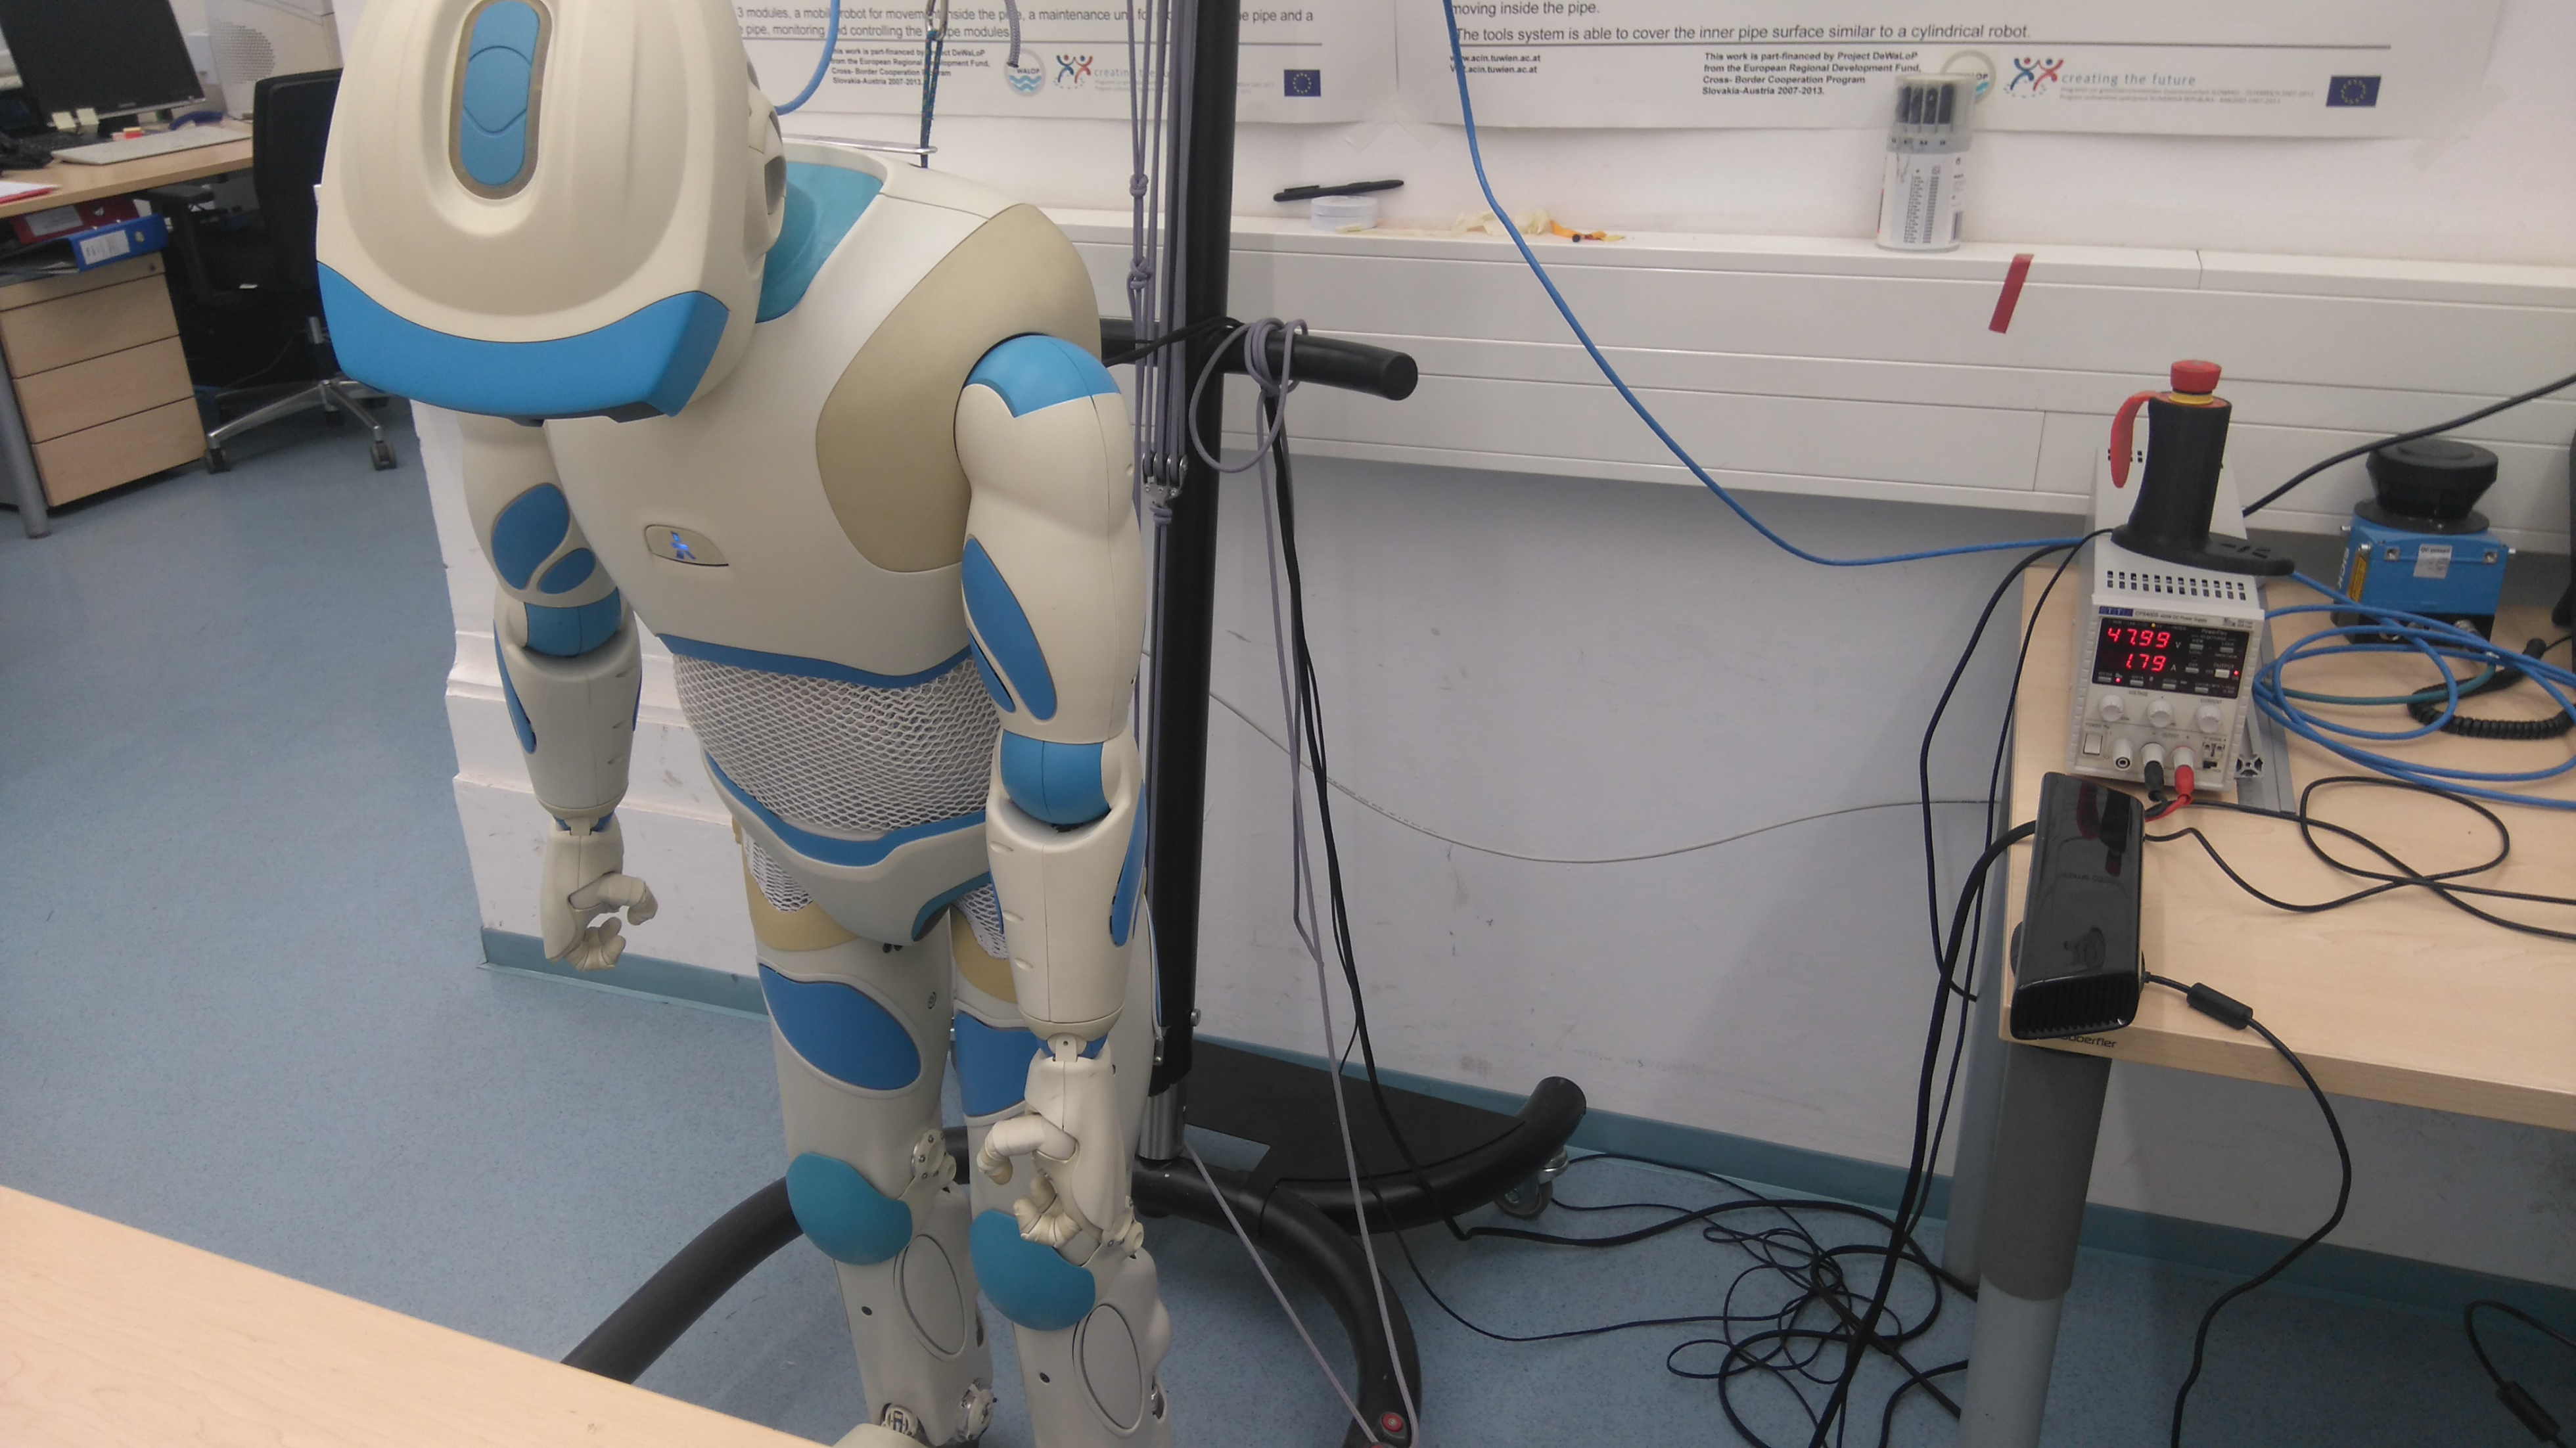
\includegraphics[width=\textwidth]{images/camera_side.eps}
        \caption{Next to the robot \label{fig:camera_side}}
\end{subfigure}
~
\begin{subfigure}[r]{0.48\textwidth}
\centering
		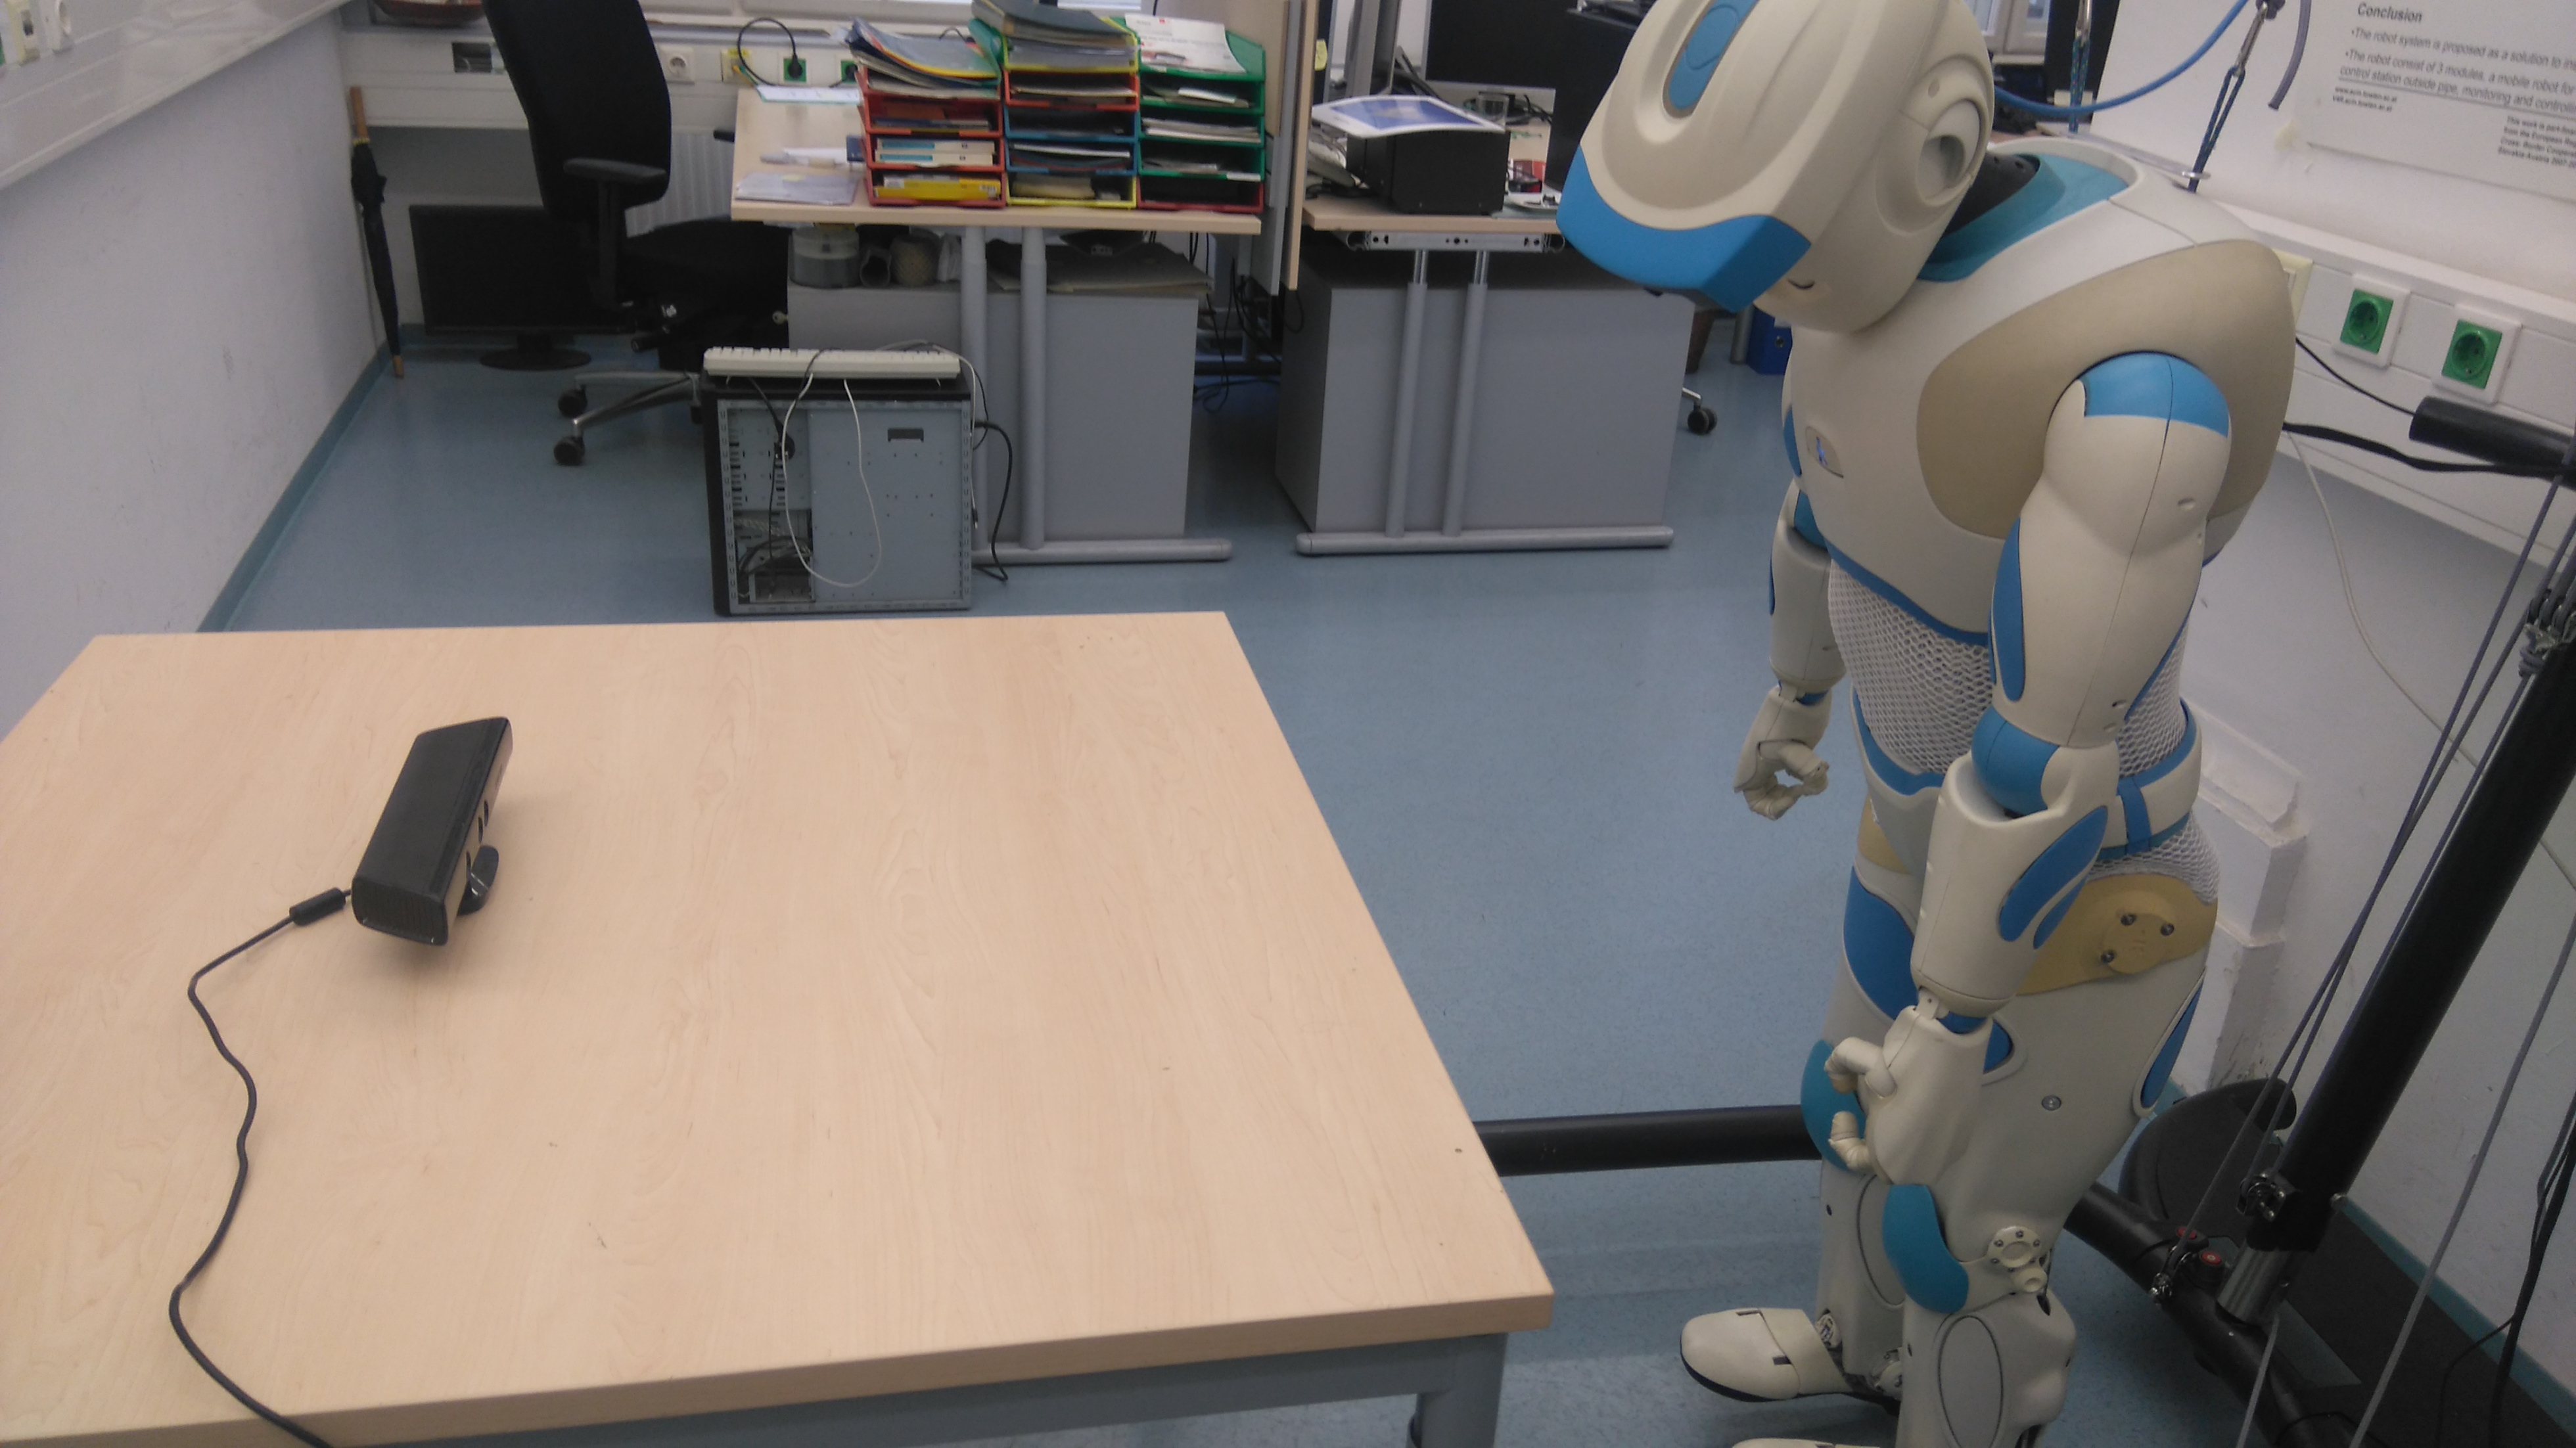
\includegraphics[width=\textwidth]{images/camera_front.eps}
        \caption{In front of the robot \label{fig:camera_front}}
\end{subfigure}
\caption{Orientations of the \texttt{camera\_link} respect to the robot \texttt{base\_link}}
\end{figure}

It should be stated that to let know the camera position to the simulator and others part of the package is used a separated thread. This one is in charge of publishing the position of the camera on \texttt{TF} when this is available. Moreover, if currently is not using a real camera it publishes the pose of the camera optical frame according to REP 103 \cite{Foote}, which is used to get the position of the object, as explained in \ref{sec:design_object_position}.

\subsection{Use of pre-known distance}
\label{sec:pre-known_distance}
In an environment where we can know the position of the camera respect to a link of the robot, use this way is a good option. Therefore we only need to set the configuration in the \texttt{romeo\_grasper.yaml} file. So with the \texttt{camera\_ref\_frame\_id} parameter we set the link used as reference and with \texttt{camera\_pose\_x}/\texttt{y}/\texttt{z} specify the coordinates where is the camera. However, we have to take in account that the orientation for this parameters is the \texttt{base\_link} orientation. That is done in that way to facilitate the user to take the coordinates.

Therefore, the process to calculate the position of the camera is, as described in Equation \eqref{eq:calc_camera_pose_pre-known}, taking position of the reference link in \texttt{base\_link} coordinates and adding the values of the parameters \texttt{camera\_pose\_x}$/$\texttt{y}$/$\texttt{z}.

\begin{equation}\label{eq:calc_camera_pose_pre-known}
P_{base}^{cam} = P_{base}^{link} + \begin{pmatrix}
camera\_pose\_x \\
camera\_pose\_y \\
camera\_pose\_z \\
\end{pmatrix} = P_{base}^{link} + \left( P_{base}^{cam} - P_{base}^{link} \right)
\end{equation}

Moreover, optionally we can set the orientation transformation from \texttt{base\_link} to \texttt{camera\_link} in RPY using the parameters \texttt{camera\_pose\_roll}/\texttt{pitch}/\texttt{yaw}. Therefore the $S_{base}^{cam}$ matrix is calculated with these parameters or, in case they don't exist, use the initial assumption. Finally, the transformation between \texttt{camera\_link} and \texttt{base\_link} is expressed like Equation \eqref{eq:trans_base_camera_pre-known}

\begin{equation}\label{eq:trans_base_camera_pre-known}
T_{base}^{cam} = \begin{pmatrix}[ccc|c]
 &  &  & \\
 & S_{base}^{cam} & & P_{base}^{cam} \\
 &  &  & \\ \hline
0 & 0 & 0 & 1
\end{pmatrix}
\end{equation}

An overview of the flow sequence done by the package in order to get this transformation is described in Figure \ref{fig:flow_camera_preknown}.

\begin{figure}[h]
\centering
% Graphic for TeX using PGF
% Title: /home/lluis/Escritorio/TFM/Informe/images/pose_preknown.dia
% Creator: Dia v0.97.2
% CreationDate: Wed May 18 16:52:55 2016
% For: lluis
% \usepackage{tikz}
% The following commands are not supported in PSTricks at present
% We define them conditionally, so when they are implemented,
% this pgf file will use them.
\ifx\du\undefined
  \newlength{\du}
\fi
\setlength{\du}{15\unitlength}
\begin{tikzpicture}
\pgftransformxscale{1.000000}
\pgftransformyscale{-1.000000}
\definecolor{dialinecolor}{rgb}{0.000000, 0.000000, 0.000000}
\pgfsetstrokecolor{dialinecolor}
\definecolor{dialinecolor}{rgb}{1.000000, 1.000000, 1.000000}
\pgfsetfillcolor{dialinecolor}
\definecolor{dialinecolor}{rgb}{0.678431, 0.847059, 0.901961}
\pgfsetfillcolor{dialinecolor}
\fill (18.180100\du,5.089170\du)--(18.180100\du,6.989170\du)--(23.657600\du,6.989170\du)--(23.657600\du,5.089170\du)--cycle;
\pgfsetlinewidth{0.100000\du}
\pgfsetdash{}{0pt}
\pgfsetdash{}{0pt}
\pgfsetmiterjoin
\definecolor{dialinecolor}{rgb}{0.000000, 0.000000, 0.000000}
\pgfsetstrokecolor{dialinecolor}
\draw (18.180100\du,5.089170\du)--(18.180100\du,6.989170\du)--(23.657600\du,6.989170\du)--(23.657600\du,5.089170\du)--cycle;
% setfont left to latex
\definecolor{dialinecolor}{rgb}{0.000000, 0.000000, 0.000000}
\pgfsetstrokecolor{dialinecolor}
\node at (20.918850\du,6.234170\du){Start function};
\definecolor{dialinecolor}{rgb}{1.000000, 0.752941, 0.796078}
\pgfsetfillcolor{dialinecolor}
\fill (20.885182\du,8.248320\du)--(25.276642\du,12.043682\du)--(20.885182\du,15.839044\du)--(16.493722\du,12.043682\du)--cycle;
\pgfsetlinewidth{0.100000\du}
\pgfsetdash{}{0pt}
\pgfsetdash{}{0pt}
\pgfsetmiterjoin
\definecolor{dialinecolor}{rgb}{0.000000, 0.000000, 0.000000}
\pgfsetstrokecolor{dialinecolor}
\draw (20.885182\du,8.248320\du)--(25.276642\du,12.043682\du)--(20.885182\du,15.839044\du)--(16.493722\du,12.043682\du)--cycle;
% setfont left to latex
\definecolor{dialinecolor}{rgb}{0.000000, 0.000000, 0.000000}
\pgfsetstrokecolor{dialinecolor}
\node at (20.885182\du,11.438682\du){Are thera all};
% setfont left to latex
\definecolor{dialinecolor}{rgb}{0.000000, 0.000000, 0.000000}
\pgfsetstrokecolor{dialinecolor}
\node at (20.885182\du,12.238682\du){camera\_pose};
% setfont left to latex
\definecolor{dialinecolor}{rgb}{0.000000, 0.000000, 0.000000}
\pgfsetstrokecolor{dialinecolor}
\node at (20.885182\du,13.038682\du){parameters?};
\definecolor{dialinecolor}{rgb}{1.000000, 0.752941, 0.796078}
\pgfsetfillcolor{dialinecolor}
\fill (30.729616\du,9.098220\du)--(34.241132\du,12.039864\du)--(30.729616\du,14.981508\du)--(27.218100\du,12.039864\du)--cycle;
\pgfsetlinewidth{0.100000\du}
\pgfsetdash{}{0pt}
\pgfsetdash{}{0pt}
\pgfsetmiterjoin
\definecolor{dialinecolor}{rgb}{0.000000, 0.000000, 0.000000}
\pgfsetstrokecolor{dialinecolor}
\draw (30.729616\du,9.098220\du)--(34.241132\du,12.039864\du)--(30.729616\du,14.981508\du)--(27.218100\du,12.039864\du)--cycle;
% setfont left to latex
\definecolor{dialinecolor}{rgb}{0.000000, 0.000000, 0.000000}
\pgfsetstrokecolor{dialinecolor}
\node at (30.729616\du,11.834864\du){Is tracking};
% setfont left to latex
\definecolor{dialinecolor}{rgb}{0.000000, 0.000000, 0.000000}
\pgfsetstrokecolor{dialinecolor}
\node at (30.729616\du,12.634864\du){ON?};
\definecolor{dialinecolor}{rgb}{0.678431, 0.847059, 0.901961}
\pgfsetfillcolor{dialinecolor}
\fill (26.106200\du,16.410800\du)--(26.106200\du,18.310800\du)--(35.343700\du,18.310800\du)--(35.343700\du,16.410800\du)--cycle;
\pgfsetlinewidth{0.100000\du}
\pgfsetdash{}{0pt}
\pgfsetdash{}{0pt}
\pgfsetmiterjoin
\definecolor{dialinecolor}{rgb}{0.000000, 0.000000, 0.000000}
\pgfsetstrokecolor{dialinecolor}
\draw (26.106200\du,16.410800\du)--(26.106200\du,18.310800\du)--(35.343700\du,18.310800\du)--(35.343700\du,16.410800\du)--cycle;
% setfont left to latex
\definecolor{dialinecolor}{rgb}{0.000000, 0.000000, 0.000000}
\pgfsetstrokecolor{dialinecolor}
\node at (30.724950\du,17.555800\du){Change to tracking mode};
\pgfsetlinewidth{0.100000\du}
\pgfsetdash{}{0pt}
\pgfsetdash{}{0pt}
\pgfsetbuttcap
\pgfsetmiterjoin
\pgfsetlinewidth{0.100000\du}
\pgfsetbuttcap
\pgfsetmiterjoin
\pgfsetdash{}{0pt}
\definecolor{dialinecolor}{rgb}{1.000000, 0.878431, 0.650980}
\pgfsetfillcolor{dialinecolor}
\pgfpathmoveto{\pgfpoint{38.070400\du}{9.950000\du}}
\pgfpathlineto{\pgfpoint{43.477900\du}{9.950000\du}}
\pgfpathlineto{\pgfpoint{44.559400\du}{10.950000\du}}
\pgfpathlineto{\pgfpoint{43.477900\du}{11.950000\du}}
\pgfpathlineto{\pgfpoint{38.070400\du}{11.950000\du}}
\pgfpathlineto{\pgfpoint{36.988900\du}{10.950000\du}}
\pgfpathlineto{\pgfpoint{38.070400\du}{9.950000\du}}
\pgfusepath{fill}
\definecolor{dialinecolor}{rgb}{0.000000, 0.000000, 0.000000}
\pgfsetstrokecolor{dialinecolor}
\pgfpathmoveto{\pgfpoint{38.070400\du}{9.950000\du}}
\pgfpathlineto{\pgfpoint{43.477900\du}{9.950000\du}}
\pgfpathlineto{\pgfpoint{44.559400\du}{10.950000\du}}
\pgfpathlineto{\pgfpoint{43.477900\du}{11.950000\du}}
\pgfpathlineto{\pgfpoint{38.070400\du}{11.950000\du}}
\pgfpathlineto{\pgfpoint{36.988900\du}{10.950000\du}}
\pgfpathlineto{\pgfpoint{38.070400\du}{9.950000\du}}
\pgfusepath{stroke}
% setfont left to latex
\definecolor{dialinecolor}{rgb}{0.000000, 0.000000, 0.000000}
\pgfsetstrokecolor{dialinecolor}
\node at (40.774150\du,10.750000\du){Wait for params};
% setfont left to latex
\definecolor{dialinecolor}{rgb}{0.000000, 0.000000, 0.000000}
\pgfsetstrokecolor{dialinecolor}
\node at (40.774150\du,11.550000\du){or tracking ON};
\definecolor{dialinecolor}{rgb}{0.678431, 0.847059, 0.901961}
\pgfsetfillcolor{dialinecolor}
\fill (36.702600\du,12.840500\du)--(36.702600\du,15.540500\du)--(44.875100\du,15.540500\du)--(44.875100\du,12.840500\du)--cycle;
\pgfsetlinewidth{0.100000\du}
\pgfsetdash{}{0pt}
\pgfsetdash{}{0pt}
\pgfsetmiterjoin
\definecolor{dialinecolor}{rgb}{0.000000, 0.000000, 0.000000}
\pgfsetstrokecolor{dialinecolor}
\draw (36.702600\du,12.840500\du)--(36.702600\du,15.540500\du)--(44.875100\du,15.540500\du)--(44.875100\du,12.840500\du)--cycle;
% setfont left to latex
\definecolor{dialinecolor}{rgb}{0.000000, 0.000000, 0.000000}
\pgfsetstrokecolor{dialinecolor}
\node at (40.788850\du,13.985500\du){Check for params and};
% setfont left to latex
\definecolor{dialinecolor}{rgb}{0.000000, 0.000000, 0.000000}
\pgfsetstrokecolor{dialinecolor}
\node at (40.788850\du,14.785500\du){load tracking boolean};
\definecolor{dialinecolor}{rgb}{1.000000, 0.752941, 0.796078}
\pgfsetfillcolor{dialinecolor}
\fill (40.684416\du,16.987800\du)--(44.195932\du,19.929444\du)--(40.684416\du,22.871088\du)--(37.172900\du,19.929444\du)--cycle;
\pgfsetlinewidth{0.100000\du}
\pgfsetdash{}{0pt}
\pgfsetdash{}{0pt}
\pgfsetmiterjoin
\definecolor{dialinecolor}{rgb}{0.000000, 0.000000, 0.000000}
\pgfsetstrokecolor{dialinecolor}
\draw (40.684416\du,16.987800\du)--(44.195932\du,19.929444\du)--(40.684416\du,22.871088\du)--(37.172900\du,19.929444\du)--cycle;
% setfont left to latex
\definecolor{dialinecolor}{rgb}{0.000000, 0.000000, 0.000000}
\pgfsetstrokecolor{dialinecolor}
\node at (40.684416\du,19.724444\du){Is tracking};
% setfont left to latex
\definecolor{dialinecolor}{rgb}{0.000000, 0.000000, 0.000000}
\pgfsetstrokecolor{dialinecolor}
\node at (40.684416\du,20.524444\du){ON?};
\definecolor{dialinecolor}{rgb}{0.678431, 0.847059, 0.901961}
\pgfsetfillcolor{dialinecolor}
\fill (17.758400\du,19.967600\du)--(17.758400\du,21.867600\du)--(24.028400\du,21.867600\du)--(24.028400\du,19.967600\du)--cycle;
\pgfsetlinewidth{0.100000\du}
\pgfsetdash{}{0pt}
\pgfsetdash{}{0pt}
\pgfsetmiterjoin
\definecolor{dialinecolor}{rgb}{0.000000, 0.000000, 0.000000}
\pgfsetstrokecolor{dialinecolor}
\draw (17.758400\du,19.967600\du)--(17.758400\du,21.867600\du)--(24.028400\du,21.867600\du)--(24.028400\du,19.967600\du)--cycle;
% setfont left to latex
\definecolor{dialinecolor}{rgb}{0.000000, 0.000000, 0.000000}
\pgfsetstrokecolor{dialinecolor}
\node at (20.893400\du,21.112600\du){Apply equations};
\pgfsetlinewidth{0.100000\du}
\pgfsetdash{}{0pt}
\pgfsetdash{}{0pt}
\pgfsetmiterjoin
\pgfsetbuttcap
{
\definecolor{dialinecolor}{rgb}{0.000000, 0.000000, 0.000000}
\pgfsetfillcolor{dialinecolor}
% was here!!!
\pgfsetarrowsend{stealth}
{\pgfsetcornersarced{\pgfpoint{0.000000\du}{0.000000\du}}\definecolor{dialinecolor}{rgb}{0.000000, 0.000000, 0.000000}
\pgfsetstrokecolor{dialinecolor}
\draw (40.684400\du,22.871100\du)--(40.684400\du,23.337700\du)--(35.954000\du,23.337700\du)--(35.954000\du,15.370200\du)--(33.034400\du,15.370200\du)--(33.034400\du,16.410800\du);
}}
\pgfsetlinewidth{0.100000\du}
\pgfsetdash{}{0pt}
\pgfsetdash{}{0pt}
\pgfsetmiterjoin
\pgfsetbuttcap
{
\definecolor{dialinecolor}{rgb}{0.000000, 0.000000, 0.000000}
\pgfsetfillcolor{dialinecolor}
% was here!!!
\pgfsetarrowsend{stealth}
{\pgfsetcornersarced{\pgfpoint{0.000000\du}{0.000000\du}}\definecolor{dialinecolor}{rgb}{0.000000, 0.000000, 0.000000}
\pgfsetstrokecolor{dialinecolor}
\draw (44.196000\du,19.929500\du)--(45.229500\du,19.929500\du)--(45.229500\du,23.900000\du)--(34.750000\du,23.900000\du)--(34.750000\du,18.997200\du)--(22.460900\du,18.997200\du)--(22.460900\du,19.967600\du);
}}
\pgfsetlinewidth{0.100000\du}
\pgfsetdash{}{0pt}
\pgfsetdash{}{0pt}
\pgfsetbuttcap
{
\definecolor{dialinecolor}{rgb}{0.000000, 0.000000, 0.000000}
\pgfsetfillcolor{dialinecolor}
% was here!!!
\pgfsetarrowsend{stealth}
\definecolor{dialinecolor}{rgb}{0.000000, 0.000000, 0.000000}
\pgfsetstrokecolor{dialinecolor}
\draw (40.774100\du,11.950000\du)--(40.788900\du,12.840500\du);
}
\pgfsetlinewidth{0.100000\du}
\pgfsetdash{}{0pt}
\pgfsetdash{}{0pt}
\pgfsetmiterjoin
\pgfsetbuttcap
{
\definecolor{dialinecolor}{rgb}{0.000000, 0.000000, 0.000000}
\pgfsetfillcolor{dialinecolor}
% was here!!!
\pgfsetarrowsend{stealth}
{\pgfsetcornersarced{\pgfpoint{0.000000\du}{0.000000\du}}\definecolor{dialinecolor}{rgb}{0.000000, 0.000000, 0.000000}
\pgfsetstrokecolor{dialinecolor}
\draw (36.702600\du,14.190500\du)--(35.652600\du,14.190500\du)--(35.652600\du,10.950000\du)--(36.988900\du,10.950000\du);
}}
\pgfsetlinewidth{0.100000\du}
\pgfsetdash{}{0pt}
\pgfsetdash{}{0pt}
\pgfsetmiterjoin
\pgfsetbuttcap
{
\definecolor{dialinecolor}{rgb}{0.000000, 0.000000, 0.000000}
\pgfsetfillcolor{dialinecolor}
% was here!!!
\pgfsetarrowsend{stealth}
{\pgfsetcornersarced{\pgfpoint{0.000000\du}{0.000000\du}}\definecolor{dialinecolor}{rgb}{0.000000, 0.000000, 0.000000}
\pgfsetstrokecolor{dialinecolor}
\draw (44.559400\du,10.950000\du)--(45.764700\du,10.950000\du)--(45.764700\du,16.000000\du)--(40.684400\du,16.000000\du)--(40.684400\du,16.987800\du);
}}
\pgfsetlinewidth{0.100000\du}
\pgfsetdash{}{0pt}
\pgfsetdash{}{0pt}
\pgfsetbuttcap
{
\definecolor{dialinecolor}{rgb}{0.000000, 0.000000, 0.000000}
\pgfsetfillcolor{dialinecolor}
% was here!!!
\pgfsetarrowsend{stealth}
\definecolor{dialinecolor}{rgb}{0.000000, 0.000000, 0.000000}
\pgfsetstrokecolor{dialinecolor}
\draw (30.729600\du,14.981500\du)--(30.725000\du,16.410800\du);
}
\pgfsetlinewidth{0.100000\du}
\pgfsetdash{}{0pt}
\pgfsetdash{}{0pt}
\pgfsetmiterjoin
\pgfsetbuttcap
{
\definecolor{dialinecolor}{rgb}{0.000000, 0.000000, 0.000000}
\pgfsetfillcolor{dialinecolor}
% was here!!!
\pgfsetarrowsend{stealth}
{\pgfsetcornersarced{\pgfpoint{0.000000\du}{0.000000\du}}\definecolor{dialinecolor}{rgb}{0.000000, 0.000000, 0.000000}
\pgfsetstrokecolor{dialinecolor}
\draw (34.241100\du,12.039900\du)--(34.718600\du,12.039900\du)--(34.718600\du,8.900000\du)--(40.774100\du,8.900000\du)--(40.774100\du,9.950000\du);
}}
\pgfsetlinewidth{0.100000\du}
\pgfsetdash{}{0pt}
\pgfsetdash{}{0pt}
\pgfsetbuttcap
{
\definecolor{dialinecolor}{rgb}{0.000000, 0.000000, 0.000000}
\pgfsetfillcolor{dialinecolor}
% was here!!!
\pgfsetarrowsend{stealth}
\definecolor{dialinecolor}{rgb}{0.000000, 0.000000, 0.000000}
\pgfsetstrokecolor{dialinecolor}
\draw (20.885182\du,15.839044\du)--(20.893400\du,19.967600\du);
}
\pgfsetlinewidth{0.100000\du}
\pgfsetdash{}{0pt}
\pgfsetdash{}{0pt}
\pgfsetbuttcap
{
\definecolor{dialinecolor}{rgb}{0.000000, 0.000000, 0.000000}
\pgfsetfillcolor{dialinecolor}
% was here!!!
\pgfsetarrowsend{stealth}
\definecolor{dialinecolor}{rgb}{0.000000, 0.000000, 0.000000}
\pgfsetstrokecolor{dialinecolor}
\draw (25.276642\du,12.043682\du)--(27.218100\du,12.039900\du);
}
\pgfsetlinewidth{0.100000\du}
\pgfsetdash{}{0pt}
\pgfsetdash{}{0pt}
\pgfsetbuttcap
{
\definecolor{dialinecolor}{rgb}{0.000000, 0.000000, 0.000000}
\pgfsetfillcolor{dialinecolor}
% was here!!!
\pgfsetarrowsend{stealth}
\definecolor{dialinecolor}{rgb}{0.000000, 0.000000, 0.000000}
\pgfsetstrokecolor{dialinecolor}
\draw (20.918850\du,6.989170\du)--(20.885182\du,8.248320\du);
}
\definecolor{dialinecolor}{rgb}{0.631373, 0.862745, 0.631373}
\pgfsetfillcolor{dialinecolor}
\fill (16.575400\du,26.280200\du)--(16.575400\du,28.180200\du)--(25.252900\du,28.180200\du)--(25.252900\du,26.280200\du)--cycle;
\pgfsetlinewidth{0.100000\du}
\pgfsetdash{}{0pt}
\pgfsetdash{}{0pt}
\pgfsetmiterjoin
\definecolor{dialinecolor}{rgb}{0.000000, 0.000000, 0.000000}
\pgfsetstrokecolor{dialinecolor}
\draw (16.575400\du,26.280200\du)--(16.575400\du,28.180200\du)--(25.252900\du,28.180200\du)--(25.252900\du,26.280200\du)--cycle;
% setfont left to latex
\definecolor{dialinecolor}{rgb}{0.000000, 0.000000, 0.000000}
\pgfsetstrokecolor{dialinecolor}
\node at (20.914150\du,27.425200\du){Publish transform on TF};
\definecolor{dialinecolor}{rgb}{0.678431, 0.847059, 0.901961}
\pgfsetfillcolor{dialinecolor}
\fill (16.428800\du,23.080200\du)--(16.428800\du,24.980200\du)--(25.403800\du,24.980200\du)--(25.403800\du,23.080200\du)--cycle;
\pgfsetlinewidth{0.100000\du}
\pgfsetdash{}{0pt}
\pgfsetdash{}{0pt}
\pgfsetmiterjoin
\definecolor{dialinecolor}{rgb}{0.000000, 0.000000, 0.000000}
\pgfsetstrokecolor{dialinecolor}
\draw (16.428800\du,23.080200\du)--(16.428800\du,24.980200\du)--(25.403800\du,24.980200\du)--(25.403800\du,23.080200\du)--cycle;
% setfont left to latex
\definecolor{dialinecolor}{rgb}{0.000000, 0.000000, 0.000000}
\pgfsetstrokecolor{dialinecolor}
\node at (20.916300\du,24.225200\du){Create bloc on simulator};
\pgfsetlinewidth{0.100000\du}
\pgfsetdash{}{0pt}
\pgfsetdash{}{0pt}
\pgfsetbuttcap
{
\definecolor{dialinecolor}{rgb}{0.000000, 0.000000, 0.000000}
\pgfsetfillcolor{dialinecolor}
% was here!!!
\pgfsetarrowsend{stealth}
\definecolor{dialinecolor}{rgb}{0.000000, 0.000000, 0.000000}
\pgfsetstrokecolor{dialinecolor}
\draw (20.916300\du,24.980200\du)--(20.915106\du,26.229895\du);
}
\pgfsetlinewidth{0.100000\du}
\pgfsetdash{}{0pt}
\pgfsetdash{}{0pt}
\pgfsetbuttcap
{
\definecolor{dialinecolor}{rgb}{0.000000, 0.000000, 0.000000}
\pgfsetfillcolor{dialinecolor}
% was here!!!
\pgfsetarrowsend{stealth}
\definecolor{dialinecolor}{rgb}{0.000000, 0.000000, 0.000000}
\pgfsetstrokecolor{dialinecolor}
\draw (20.903992\du,21.917855\du)--(20.916300\du,23.080200\du);
}
% setfont left to latex
\definecolor{dialinecolor}{rgb}{0.000000, 0.000000, 0.000000}
\pgfsetstrokecolor{dialinecolor}
\node[anchor=west] at (20.739952\du,16.334263\du){Yes};
% setfont left to latex
\definecolor{dialinecolor}{rgb}{0.000000, 0.000000, 0.000000}
\pgfsetstrokecolor{dialinecolor}
\node[anchor=west] at (25.019432\du,11.633318\du){No};
% setfont left to latex
\definecolor{dialinecolor}{rgb}{0.000000, 0.000000, 0.000000}
\pgfsetstrokecolor{dialinecolor}
\node[anchor=west] at (33.363253\du,11.304453\du){No};
% setfont left to latex
\definecolor{dialinecolor}{rgb}{0.000000, 0.000000, 0.000000}
\pgfsetstrokecolor{dialinecolor}
\node[anchor=west] at (43.870708\du,19.385732\du){No};
% setfont left to latex
\definecolor{dialinecolor}{rgb}{0.000000, 0.000000, 0.000000}
\pgfsetstrokecolor{dialinecolor}
\node[anchor=west] at (30.512588\du,15.468495\du){Yes};
% setfont left to latex
\definecolor{dialinecolor}{rgb}{0.000000, 0.000000, 0.000000}
\pgfsetstrokecolor{dialinecolor}
\node[anchor=west] at (38.570004\du,22.838484\du){Yes};
% setfont left to latex
\definecolor{dialinecolor}{rgb}{0.000000, 0.000000, 0.000000}
\pgfsetstrokecolor{dialinecolor}
\node[anchor=west] at (44.619650\du,10.708457\du){};
\end{tikzpicture}

\caption{Process of having camera position using pre-known distance \label{fig:flow_camera_preknown}}
\end{figure}

\subsection{Use of visual recognition}
\label{sec:visual-recognition}

The original idea of this method is that wouldn't be necessary the help of the user to get the camera position. So the package should recognise one or more parts of the robot. Then, it should calculate the position and orientation of the camera knowing the position and orientation\footnote{The use of the orientation of a robot part depends on the approach used.} from the \texttt{camera\_link} reference and from the \texttt{base\_link} reference. For now, this initial idea is not totally implemented due to difficulties to recognise parts of the robot, as mentioned in Section \ref{sec:positioning_camera}, and for others problems explained later.

In order to be able to get the pose of the links of the robot is used a modeled object with a special offset and easy to recognised for the software. This object is placed next to the link of the robot in a precise location, as showed on Figure \ref{fig:modeled_object_offset}, so the final origin of the object is established on the link origin. This modeled object, when it's initialised must have boolean \texttt{is\_reference\_object} with value \texttt{true} to work properly.

\begin{figure}
\centering
\includegraphics[scale=1]{images/modeled_object_offset.eps}
\caption{Position change due to the offset of the modeled object.\label{fig:modeled_object_offset}}
\end{figure}

Below are explained the three different approaches done for this method. Although, only the first one is implemented in the package, the others are prepared in the Matlab files on the directory \texttt{data$/$matlab$/$}.

\vspace{-10pt}
\subsubsection{(1) Using only one link}

In this case, is used the assumption of having the camera next to or in front of the robot as a final orientation. Therefore, the only unknown variable is the camera position on base reference, $P_{base}^{cam}$. So as to solve this is needed the position of a link on camera reference, $P_{cam}^{link}$, that is known also on base reference, $P_{base}^{link}$. Finally the Equation \eqref{eq:camera_pose_visual_point} is the one to solve.

\vspace{-10pt}
\begin{equation}\label{eq:camera_pose_visual_point}
P_{base}^{cam} - P_{base}^{link} + S_{base}^{cam} \cdot P_{cam}^{link} = 0
\end{equation}

\vspace{-20pt}
\subsubsection{(2) Using three links}

On the other hand, this case only used the assumption of the orientation to have a seed to solve the problem. The idea of this way is to implement the resolution of an optimisation problem with non-linear constraints to have an exact position and orientation of the camera.

The equation that have to be minimized are Equation \eqref{eq:camera_pose_visual_point}, for every link, and Equation 
\eqref{eq:camera_pose_visual_vector}, for two combination of the three links.\footnote{Only two combination of Equation \eqref{eq:camera_pose_visual_vector} because the third one is linear dependent of the other two.} Therefore, the error of every equation is put as absolute value and introduce in the minimization function. 

Moreover, the solution have three non-linear constraints: the three axis of the orientation should be perpendicular between them. The axis of the orientation are the unitary vectors of the columns of matrix $S_{base}^{cam}$. Therefore, the constraints are Equation \eqref{eq:camera_pose_visual_perpendicular}, for every combination of the axis. 

\begin{equation}\label{eq:camera_pose_visual_vector}
\left( \overrightarrow{P_iP_j} \right)_{base} - S_{base}^{cam} \left( \overrightarrow{P_iP_j} \right)_{cam} = 0  \quad \quad \quad \forall i \neq j \quad \quad i,j=\left[ link_1,link_2,link_3 \right]
\end{equation}
\begin{equation}\label{eq:camera_pose_visual_perpendicular}
<v_i , v_j > = 0 \quad \quad \quad \forall i \neq j \quad \quad i,j=\left[x,y,z\right]
\end{equation}

The reason to use three link for this case is that a minimum of 12 equation are required to determine the 12 variables (3 for the camera position and 9 for the orientation). Using three links we get 15 equations and 3 non-linear constraints. Otherwise with two link we would have 9 equation and 3 non-linear constraints, which is not enough.

As said previously, the fact of having the camera in front or next to the robot is used as a seed. So the depending of the case is used the matrix from Equation \eqref{eq:matrix_rot_side} or from Equation \eqref{eq:matrix_rot_front}. Furthermore, for the position there are also seeds, these are extracted experimentally.

Finally mention that in Matlab is used the algorithm \texttt{GlobalSearch} because it allows non-linear constraints and also search in a big range of solutions and is not only trying from the given seed. 

\vspace{-10pt}
\subsubsection{(3) Using multiples transformations}

The V4R software, apart from giving the position of the object, gives the orientation. So instead of only using the position of the link placing the reference object at a certain place, we could use also the orientation of the object. Therefore, we could discover the position and orientation of the camera placing the object in a precise position and orientation from the known link. In order to do that we should know: (1) the transform from object to link reference, because of that reference object is placed by us; (2) the transform from link to base, provided by the model of the robot; (3) the transform from camera to object, known by using the information of the V4R software. With all this information we could have the transformation from camera to base, as showed in Equation \eqref{eq:camera_pose_trans}, so finally get position and orientation of the camera.

\begin{equation}\label{eq:camera_pose_trans}
T_{base}^{cam} = T_{base}^{link} \cdot T_{link}^{obj} \cdot T_{obj}^{cam}
\end{equation} 

\section{Planning and execution of trajectory}

A brief description of this part is in Section \ref{sec:design_move_hand}. Firstly, before planning the ROS parameters named as runtime parameters are constantly updated. And secondly, is needed to accomplish the following conditions:

\begin{itemize}
\item The modeled object which should be grasp has the position updated.
\item The position of the object is a new one which has not been processed.
\item Be sure is not doing other processes that can effect the planning and execution
\end{itemize}

After that, is time to start with the planning and execute function, an overview can be seen in Figure \ref{fig:plan_execute_function_flow}. Therefore, below is explained in more detail some parts of this function.

\begin{figure}[!h]
\centering
% Graphic for TeX using PGF
% Title: /home/lluis/Escritorio/TFM/Informe/images/plan_execute_function_flow.dia
% Creator: Dia v0.97.2
% CreationDate: Fri May 27 10:02:38 2016
% For: lluis
% \usepackage{tikz}
% The following commands are not supported in PSTricks at present
% We define them conditionally, so when they are implemented,
% this pgf file will use them.
\ifx\du\undefined
  \newlength{\du}
\fi
\setlength{\du}{15\unitlength}
\begin{tikzpicture}
\pgftransformxscale{1.000000}
\pgftransformyscale{-1.000000}
\definecolor{dialinecolor}{rgb}{0.000000, 0.000000, 0.000000}
\pgfsetstrokecolor{dialinecolor}
\definecolor{dialinecolor}{rgb}{1.000000, 1.000000, 1.000000}
\pgfsetfillcolor{dialinecolor}
\definecolor{dialinecolor}{rgb}{0.678431, 0.847059, 0.901961}
\pgfsetfillcolor{dialinecolor}
\fill (20.123700\du,3.179680\du)--(20.123700\du,5.879680\du)--(27.376200\du,5.879680\du)--(27.376200\du,3.179680\du)--cycle;
\pgfsetlinewidth{0.100000\du}
\pgfsetdash{}{0pt}
\pgfsetdash{}{0pt}
\pgfsetmiterjoin
\definecolor{dialinecolor}{rgb}{0.000000, 0.000000, 0.000000}
\pgfsetstrokecolor{dialinecolor}
\draw (20.123700\du,3.179680\du)--(20.123700\du,5.879680\du)--(27.376200\du,5.879680\du)--(27.376200\du,3.179680\du)--cycle;
% setfont left to latex
\definecolor{dialinecolor}{rgb}{0.000000, 0.000000, 0.000000}
\pgfsetstrokecolor{dialinecolor}
\node at (23.749950\du,4.324680\du){Start planning and };
% setfont left to latex
\definecolor{dialinecolor}{rgb}{0.000000, 0.000000, 0.000000}
\pgfsetstrokecolor{dialinecolor}
\node at (23.749950\du,5.124680\du){execute function};
\definecolor{dialinecolor}{rgb}{0.678431, 0.847059, 0.901961}
\pgfsetfillcolor{dialinecolor}
\fill (29.738700\du,8.093680\du)--(29.738700\du,9.993680\du)--(36.878700\du,9.993680\du)--(36.878700\du,8.093680\du)--cycle;
\pgfsetlinewidth{0.100000\du}
\pgfsetdash{}{0pt}
\pgfsetdash{}{0pt}
\pgfsetmiterjoin
\definecolor{dialinecolor}{rgb}{0.000000, 0.000000, 0.000000}
\pgfsetstrokecolor{dialinecolor}
\draw (29.738700\du,8.093680\du)--(29.738700\du,9.993680\du)--(36.878700\du,9.993680\du)--(36.878700\du,8.093680\du)--cycle;
% setfont left to latex
\definecolor{dialinecolor}{rgb}{0.000000, 0.000000, 0.000000}
\pgfsetstrokecolor{dialinecolor}
\node at (33.308700\du,9.238680\du){Planning pre-grasp};
\definecolor{dialinecolor}{rgb}{1.000000, 0.878431, 0.650980}
\pgfsetfillcolor{dialinecolor}
\fill (23.750018\du,12.774700\du)--(27.111435\du,15.844550\du)--(23.750018\du,18.914400\du)--(20.388600\du,15.844550\du)--cycle;
\pgfsetlinewidth{0.100000\du}
\pgfsetdash{}{0pt}
\pgfsetdash{}{0pt}
\pgfsetmiterjoin
\definecolor{dialinecolor}{rgb}{0.000000, 0.000000, 0.000000}
\pgfsetstrokecolor{dialinecolor}
\draw (23.750018\du,12.774700\du)--(27.111435\du,15.844550\du)--(23.750018\du,18.914400\du)--(20.388600\du,15.844550\du)--cycle;
% setfont left to latex
\definecolor{dialinecolor}{rgb}{0.000000, 0.000000, 0.000000}
\pgfsetstrokecolor{dialinecolor}
\node at (23.750018\du,15.639550\du){Automatic};
% setfont left to latex
\definecolor{dialinecolor}{rgb}{0.000000, 0.000000, 0.000000}
\pgfsetstrokecolor{dialinecolor}
\node at (23.750018\du,16.439550\du){execution};
\definecolor{dialinecolor}{rgb}{1.000000, 0.647059, 0.000000}
\pgfsetfillcolor{dialinecolor}
\fill (30.046200\du,20.850000\du)--(30.046200\du,23.550000\du)--(36.571200\du,23.550000\du)--(36.571200\du,20.850000\du)--cycle;
\pgfsetlinewidth{0.100000\du}
\pgfsetdash{}{0pt}
\pgfsetdash{}{0pt}
\pgfsetmiterjoin
\definecolor{dialinecolor}{rgb}{0.000000, 0.000000, 0.000000}
\pgfsetstrokecolor{dialinecolor}
\draw (30.046200\du,20.850000\du)--(30.046200\du,23.550000\du)--(36.571200\du,23.550000\du)--(36.571200\du,20.850000\du)--cycle;
% setfont left to latex
\definecolor{dialinecolor}{rgb}{0.000000, 0.000000, 0.000000}
\pgfsetstrokecolor{dialinecolor}
\node at (33.308700\du,21.995000\du){Switch};
% setfont left to latex
\definecolor{dialinecolor}{rgb}{0.000000, 0.000000, 0.000000}
\pgfsetstrokecolor{dialinecolor}
\node at (33.308700\du,22.795000\du){(answer\_service)};
\definecolor{dialinecolor}{rgb}{1.000000, 0.878431, 0.650980}
\pgfsetfillcolor{dialinecolor}
\fill (33.308715\du,24.434600\du)--(35.738730\du,26.108591\du)--(33.308715\du,27.782583\du)--(30.878700\du,26.108591\du)--cycle;
\pgfsetlinewidth{0.100000\du}
\pgfsetdash{}{0pt}
\pgfsetdash{}{0pt}
\pgfsetmiterjoin
\definecolor{dialinecolor}{rgb}{0.000000, 0.000000, 0.000000}
\pgfsetstrokecolor{dialinecolor}
\draw (33.308715\du,24.434600\du)--(35.738730\du,26.108591\du)--(33.308715\du,27.782583\du)--(30.878700\du,26.108591\du)--cycle;
% setfont left to latex
\definecolor{dialinecolor}{rgb}{0.000000, 0.000000, 0.000000}
\pgfsetstrokecolor{dialinecolor}
\node at (33.308715\du,26.303591\du){Move};
\definecolor{dialinecolor}{rgb}{0.678431, 0.847059, 0.901961}
\pgfsetfillcolor{dialinecolor}
\fill (43.641800\du,25.158600\du)--(43.641800\du,27.058600\du)--(48.866800\du,27.058600\du)--(48.866800\du,25.158600\du)--cycle;
\pgfsetlinewidth{0.100000\du}
\pgfsetdash{}{0pt}
\pgfsetdash{}{0pt}
\pgfsetmiterjoin
\definecolor{dialinecolor}{rgb}{0.000000, 0.000000, 0.000000}
\pgfsetstrokecolor{dialinecolor}
\draw (43.641800\du,25.158600\du)--(43.641800\du,27.058600\du)--(48.866800\du,27.058600\du)--(48.866800\du,25.158600\du)--cycle;
% setfont left to latex
\definecolor{dialinecolor}{rgb}{0.000000, 0.000000, 0.000000}
\pgfsetstrokecolor{dialinecolor}
\node at (46.254300\du,26.303600\du){Execute Plan};
\definecolor{dialinecolor}{rgb}{1.000000, 0.878431, 0.650980}
\pgfsetfillcolor{dialinecolor}
\fill (33.308722\du,30.293100\du)--(35.815444\du,32.296031\du)--(33.308722\du,34.298962\du)--(30.802000\du,32.296031\du)--cycle;
\pgfsetlinewidth{0.100000\du}
\pgfsetdash{}{0pt}
\pgfsetdash{}{0pt}
\pgfsetmiterjoin
\definecolor{dialinecolor}{rgb}{0.000000, 0.000000, 0.000000}
\pgfsetstrokecolor{dialinecolor}
\draw (33.308722\du,30.293100\du)--(35.815444\du,32.296031\du)--(33.308722\du,34.298962\du)--(30.802000\du,32.296031\du)--cycle;
% setfont left to latex
\definecolor{dialinecolor}{rgb}{0.000000, 0.000000, 0.000000}
\pgfsetstrokecolor{dialinecolor}
\node at (33.308722\du,32.491031\du){Replan};
\pgfsetlinewidth{0.100000\du}
\pgfsetdash{}{0pt}
\pgfsetdash{}{0pt}
\pgfsetbuttcap
\pgfsetmiterjoin
\pgfsetlinewidth{0.100000\du}
\pgfsetbuttcap
\pgfsetmiterjoin
\pgfsetdash{}{0pt}
\definecolor{dialinecolor}{rgb}{1.000000, 0.752941, 0.796078}
\pgfsetfillcolor{dialinecolor}
\pgfpathmoveto{\pgfpoint{21.056800\du}{19.706300\du}}
\pgfpathlineto{\pgfpoint{26.464300\du}{19.706300\du}}
\pgfpathlineto{\pgfpoint{27.545800\du}{20.656300\du}}
\pgfpathlineto{\pgfpoint{26.464300\du}{21.606300\du}}
\pgfpathlineto{\pgfpoint{21.056800\du}{21.606300\du}}
\pgfpathlineto{\pgfpoint{19.975300\du}{20.656300\du}}
\pgfpathlineto{\pgfpoint{21.056800\du}{19.706300\du}}
\pgfusepath{fill}
\definecolor{dialinecolor}{rgb}{0.000000, 0.000000, 0.000000}
\pgfsetstrokecolor{dialinecolor}
\pgfpathmoveto{\pgfpoint{21.056800\du}{19.706300\du}}
\pgfpathlineto{\pgfpoint{26.464300\du}{19.706300\du}}
\pgfpathlineto{\pgfpoint{27.545800\du}{20.656300\du}}
\pgfpathlineto{\pgfpoint{26.464300\du}{21.606300\du}}
\pgfpathlineto{\pgfpoint{21.056800\du}{21.606300\du}}
\pgfpathlineto{\pgfpoint{19.975300\du}{20.656300\du}}
\pgfpathlineto{\pgfpoint{21.056800\du}{19.706300\du}}
\pgfusepath{stroke}
% setfont left to latex
\definecolor{dialinecolor}{rgb}{0.000000, 0.000000, 0.000000}
\pgfsetstrokecolor{dialinecolor}
\node at (23.760550\du,20.456300\du){Wait user's};
% setfont left to latex
\definecolor{dialinecolor}{rgb}{0.000000, 0.000000, 0.000000}
\pgfsetstrokecolor{dialinecolor}
\node at (23.760550\du,21.256300\du){service call};
\definecolor{dialinecolor}{rgb}{0.678431, 0.847059, 0.901961}
\pgfsetfillcolor{dialinecolor}
\fill (19.088700\du,22.728500\du)--(19.088700\du,24.628500\du)--(28.363700\du,24.628500\du)--(28.363700\du,22.728500\du)--cycle;
\pgfsetlinewidth{0.100000\du}
\pgfsetdash{}{0pt}
\pgfsetdash{}{0pt}
\pgfsetmiterjoin
\definecolor{dialinecolor}{rgb}{0.000000, 0.000000, 0.000000}
\pgfsetstrokecolor{dialinecolor}
\draw (19.088700\du,22.728500\du)--(19.088700\du,24.628500\du)--(28.363700\du,24.628500\du)--(28.363700\du,22.728500\du)--cycle;
% setfont left to latex
\definecolor{dialinecolor}{rgb}{0.000000, 0.000000, 0.000000}
\pgfsetstrokecolor{dialinecolor}
\node at (23.726200\du,23.873500\du){Load runtime parameters};
\definecolor{dialinecolor}{rgb}{0.847059, 0.898039, 0.898039}
\pgfsetfillcolor{dialinecolor}
\fill (28.943000\du,14.899000\du)--(28.943000\du,16.799000\du)--(37.630500\du,16.799000\du)--(37.630500\du,14.899000\du)--cycle;
\pgfsetlinewidth{0.100000\du}
\pgfsetdash{}{0pt}
\pgfsetdash{}{0pt}
\pgfsetmiterjoin
\definecolor{dialinecolor}{rgb}{0.000000, 0.000000, 0.000000}
\pgfsetstrokecolor{dialinecolor}
\draw (28.943000\du,14.899000\du)--(28.943000\du,16.799000\du)--(37.630500\du,16.799000\du)--(37.630500\du,14.899000\du)--cycle;
% setfont left to latex
\definecolor{dialinecolor}{rgb}{0.000000, 0.000000, 0.000000}
\pgfsetstrokecolor{dialinecolor}
\node at (33.286750\du,16.044000\du){answer\_service = Move};
\definecolor{dialinecolor}{rgb}{1.000000, 0.878431, 0.650980}
\pgfsetfillcolor{dialinecolor}
\fill (39.736401\du,23.712200\du)--(42.848502\du,26.108583\du)--(39.736401\du,28.504966\du)--(36.624300\du,26.108583\du)--cycle;
\pgfsetlinewidth{0.100000\du}
\pgfsetdash{}{0pt}
\pgfsetdash{}{0pt}
\pgfsetmiterjoin
\definecolor{dialinecolor}{rgb}{0.000000, 0.000000, 0.000000}
\pgfsetstrokecolor{dialinecolor}
\draw (39.736401\du,23.712200\du)--(42.848502\du,26.108583\du)--(39.736401\du,28.504966\du)--(36.624300\du,26.108583\du)--cycle;
% setfont left to latex
\definecolor{dialinecolor}{rgb}{0.000000, 0.000000, 0.000000}
\pgfsetstrokecolor{dialinecolor}
\node at (39.736401\du,26.303583\du){isPregrasp};
\definecolor{dialinecolor}{rgb}{0.847059, 0.898039, 0.898039}
\pgfsetfillcolor{dialinecolor}
\fill (43.669300\du,28.950000\du)--(43.669300\du,31.650000\du)--(48.839300\du,31.650000\du)--(48.839300\du,28.950000\du)--cycle;
\pgfsetlinewidth{0.100000\du}
\pgfsetdash{}{0pt}
\pgfsetdash{}{0pt}
\pgfsetmiterjoin
\definecolor{dialinecolor}{rgb}{0.000000, 0.000000, 0.000000}
\pgfsetstrokecolor{dialinecolor}
\draw (43.669300\du,28.950000\du)--(43.669300\du,31.650000\du)--(48.839300\du,31.650000\du)--(48.839300\du,28.950000\du)--cycle;
% setfont left to latex
\definecolor{dialinecolor}{rgb}{0.000000, 0.000000, 0.000000}
\pgfsetstrokecolor{dialinecolor}
\node at (46.254300\du,30.095000\du){isPregrasp =};
% setfont left to latex
\definecolor{dialinecolor}{rgb}{0.000000, 0.000000, 0.000000}
\pgfsetstrokecolor{dialinecolor}
\node at (46.254300\du,30.895000\du){false};
\definecolor{dialinecolor}{rgb}{1.000000, 0.878431, 0.650980}
\pgfsetfillcolor{dialinecolor}
\fill (23.750001\du,6.647300\du)--(26.862102\du,9.043683\du)--(23.750001\du,11.440066\du)--(20.637900\du,9.043683\du)--cycle;
\pgfsetlinewidth{0.100000\du}
\pgfsetdash{}{0pt}
\pgfsetdash{}{0pt}
\pgfsetmiterjoin
\definecolor{dialinecolor}{rgb}{0.000000, 0.000000, 0.000000}
\pgfsetstrokecolor{dialinecolor}
\draw (23.750001\du,6.647300\du)--(26.862102\du,9.043683\du)--(23.750001\du,11.440066\du)--(20.637900\du,9.043683\du)--cycle;
% setfont left to latex
\definecolor{dialinecolor}{rgb}{0.000000, 0.000000, 0.000000}
\pgfsetstrokecolor{dialinecolor}
\node at (23.750001\du,9.238683\du){isPregrasp};
\definecolor{dialinecolor}{rgb}{0.678431, 0.847059, 0.901961}
\pgfsetfillcolor{dialinecolor}
\fill (37.493900\du,29.350000\du)--(37.493900\du,31.250000\du)--(41.978900\du,31.250000\du)--(41.978900\du,29.350000\du)--cycle;
\pgfsetlinewidth{0.100000\du}
\pgfsetdash{}{0pt}
\pgfsetdash{}{0pt}
\pgfsetmiterjoin
\definecolor{dialinecolor}{rgb}{0.000000, 0.000000, 0.000000}
\pgfsetstrokecolor{dialinecolor}
\draw (37.493900\du,29.350000\du)--(37.493900\du,31.250000\du)--(41.978900\du,31.250000\du)--(41.978900\du,29.350000\du)--cycle;
% setfont left to latex
\definecolor{dialinecolor}{rgb}{0.000000, 0.000000, 0.000000}
\pgfsetstrokecolor{dialinecolor}
\node at (39.736400\du,30.495000\du){Picking};
\definecolor{dialinecolor}{rgb}{1.000000, 0.878431, 0.650980}
\pgfsetfillcolor{dialinecolor}
\fill (33.318335\du,35.104300\du)--(35.672370\du,36.863133\du)--(33.318335\du,38.621967\du)--(30.964300\du,36.863133\du)--cycle;
\pgfsetlinewidth{0.100000\du}
\pgfsetdash{}{0pt}
\pgfsetdash{}{0pt}
\pgfsetmiterjoin
\definecolor{dialinecolor}{rgb}{0.000000, 0.000000, 0.000000}
\pgfsetstrokecolor{dialinecolor}
\draw (33.318335\du,35.104300\du)--(35.672370\du,36.863133\du)--(33.318335\du,38.621967\du)--(30.964300\du,36.863133\du)--cycle;
% setfont left to latex
\definecolor{dialinecolor}{rgb}{0.000000, 0.000000, 0.000000}
\pgfsetstrokecolor{dialinecolor}
\node at (33.318335\du,37.058133\du){Abort};
\pgfsetlinewidth{0.100000\du}
\pgfsetdash{}{0pt}
\pgfsetdash{}{0pt}
\pgfsetbuttcap
{
\definecolor{dialinecolor}{rgb}{0.000000, 0.000000, 0.000000}
\pgfsetfillcolor{dialinecolor}
% was here!!!
\pgfsetarrowsend{stealth}
\definecolor{dialinecolor}{rgb}{0.000000, 0.000000, 0.000000}
\pgfsetstrokecolor{dialinecolor}
\draw (23.750000\du,5.879680\du)--(23.750000\du,6.647300\du);
}
\pgfsetlinewidth{0.100000\du}
\pgfsetdash{}{0pt}
\pgfsetdash{}{0pt}
\pgfsetbuttcap
{
\definecolor{dialinecolor}{rgb}{0.000000, 0.000000, 0.000000}
\pgfsetfillcolor{dialinecolor}
% was here!!!
\pgfsetarrowsend{stealth}
\definecolor{dialinecolor}{rgb}{0.000000, 0.000000, 0.000000}
\pgfsetstrokecolor{dialinecolor}
\draw (23.750000\du,11.440100\du)--(23.750000\du,12.774700\du);
}
\pgfsetlinewidth{0.100000\du}
\pgfsetdash{}{0pt}
\pgfsetdash{}{0pt}
\pgfsetbuttcap
{
\definecolor{dialinecolor}{rgb}{0.000000, 0.000000, 0.000000}
\pgfsetfillcolor{dialinecolor}
% was here!!!
\pgfsetarrowsend{stealth}
\definecolor{dialinecolor}{rgb}{0.000000, 0.000000, 0.000000}
\pgfsetstrokecolor{dialinecolor}
\draw (26.862100\du,9.043680\du)--(29.738700\du,9.043680\du);
}
\pgfsetlinewidth{0.100000\du}
\pgfsetdash{}{0pt}
\pgfsetdash{}{0pt}
\pgfsetbuttcap
{
\definecolor{dialinecolor}{rgb}{0.000000, 0.000000, 0.000000}
\pgfsetfillcolor{dialinecolor}
% was here!!!
\pgfsetarrowsend{stealth}
\definecolor{dialinecolor}{rgb}{0.000000, 0.000000, 0.000000}
\pgfsetstrokecolor{dialinecolor}
\draw (23.760600\du,21.606300\du)--(23.726200\du,22.728500\du);
}
\pgfsetlinewidth{0.100000\du}
\pgfsetdash{}{0pt}
\pgfsetdash{}{0pt}
\pgfsetbuttcap
{
\definecolor{dialinecolor}{rgb}{0.000000, 0.000000, 0.000000}
\pgfsetfillcolor{dialinecolor}
% was here!!!
\pgfsetarrowsend{stealth}
\definecolor{dialinecolor}{rgb}{0.000000, 0.000000, 0.000000}
\pgfsetstrokecolor{dialinecolor}
\draw (33.308700\du,23.550000\du)--(33.308700\du,24.434600\du);
}
\pgfsetlinewidth{0.100000\du}
\pgfsetdash{}{0pt}
\pgfsetdash{}{0pt}
\pgfsetbuttcap
{
\definecolor{dialinecolor}{rgb}{0.000000, 0.000000, 0.000000}
\pgfsetfillcolor{dialinecolor}
% was here!!!
\pgfsetarrowsend{stealth}
\definecolor{dialinecolor}{rgb}{0.000000, 0.000000, 0.000000}
\pgfsetstrokecolor{dialinecolor}
\draw (33.308700\du,27.782600\du)--(33.308700\du,30.293100\du);
}
\pgfsetlinewidth{0.100000\du}
\pgfsetdash{}{0pt}
\pgfsetdash{}{0pt}
\pgfsetbuttcap
{
\definecolor{dialinecolor}{rgb}{0.000000, 0.000000, 0.000000}
\pgfsetfillcolor{dialinecolor}
% was here!!!
\pgfsetarrowsend{stealth}
\definecolor{dialinecolor}{rgb}{0.000000, 0.000000, 0.000000}
\pgfsetstrokecolor{dialinecolor}
\draw (35.738700\du,26.108600\du)--(36.624300\du,26.108600\du);
}
\pgfsetlinewidth{0.100000\du}
\pgfsetdash{}{0pt}
\pgfsetdash{}{0pt}
\pgfsetbuttcap
{
\definecolor{dialinecolor}{rgb}{0.000000, 0.000000, 0.000000}
\pgfsetfillcolor{dialinecolor}
% was here!!!
\pgfsetarrowsend{stealth}
\definecolor{dialinecolor}{rgb}{0.000000, 0.000000, 0.000000}
\pgfsetstrokecolor{dialinecolor}
\draw (39.736400\du,28.505000\du)--(39.736400\du,29.350000\du);
}
\pgfsetlinewidth{0.100000\du}
\pgfsetdash{}{0pt}
\pgfsetdash{}{0pt}
\pgfsetbuttcap
{
\definecolor{dialinecolor}{rgb}{0.000000, 0.000000, 0.000000}
\pgfsetfillcolor{dialinecolor}
% was here!!!
\pgfsetarrowsend{stealth}
\definecolor{dialinecolor}{rgb}{0.000000, 0.000000, 0.000000}
\pgfsetstrokecolor{dialinecolor}
\draw (42.848500\du,26.108600\du)--(43.641800\du,26.108600\du);
}
\pgfsetlinewidth{0.100000\du}
\pgfsetdash{}{0pt}
\pgfsetdash{}{0pt}
\pgfsetbuttcap
{
\definecolor{dialinecolor}{rgb}{0.000000, 0.000000, 0.000000}
\pgfsetfillcolor{dialinecolor}
% was here!!!
\pgfsetarrowsend{stealth}
\definecolor{dialinecolor}{rgb}{0.000000, 0.000000, 0.000000}
\pgfsetstrokecolor{dialinecolor}
\draw (46.254300\du,27.058600\du)--(46.254300\du,28.950000\du);
}
\pgfsetlinewidth{0.100000\du}
\pgfsetdash{}{0pt}
\pgfsetdash{}{0pt}
\pgfsetmiterjoin
\pgfsetbuttcap
{
\definecolor{dialinecolor}{rgb}{0.000000, 0.000000, 0.000000}
\pgfsetfillcolor{dialinecolor}
% was here!!!
\pgfsetarrowsend{stealth}
{\pgfsetcornersarced{\pgfpoint{0.000000\du}{0.000000\du}}\definecolor{dialinecolor}{rgb}{0.000000, 0.000000, 0.000000}
\pgfsetstrokecolor{dialinecolor}
\draw (46.254300\du,31.650000\du)--(46.254300\du,32.297800\du)--(49.487519\du,32.297800\du)--(49.487519\du,4.529680\du)--(27.376200\du,4.529680\du);
}}
\pgfsetlinewidth{0.100000\du}
\pgfsetdash{}{0pt}
\pgfsetdash{}{0pt}
\pgfsetbuttcap
{
\definecolor{dialinecolor}{rgb}{0.000000, 0.000000, 0.000000}
\pgfsetfillcolor{dialinecolor}
% was here!!!
\pgfsetarrowsend{stealth}
\definecolor{dialinecolor}{rgb}{0.000000, 0.000000, 0.000000}
\pgfsetstrokecolor{dialinecolor}
\draw (33.308700\du,34.299000\du)--(33.318300\du,35.104300\du);
}
\pgfsetlinewidth{0.100000\du}
\pgfsetdash{}{0pt}
\pgfsetdash{}{0pt}
\pgfsetbuttcap
{
\definecolor{dialinecolor}{rgb}{0.000000, 0.000000, 0.000000}
\pgfsetfillcolor{dialinecolor}
% was here!!!
\pgfsetarrowsend{latex}
\definecolor{dialinecolor}{rgb}{0.000000, 0.000000, 0.000000}
\pgfsetstrokecolor{dialinecolor}
\draw (35.815400\du,32.296000\du)--(46.272400\du,32.285200\du);
}
\definecolor{dialinecolor}{rgb}{0.847059, 0.898039, 0.898039}
\pgfsetfillcolor{dialinecolor}
\fill (36.988900\du,35.513200\du)--(36.988900\du,38.213200\du)--(42.538900\du,38.213200\du)--(42.538900\du,35.513200\du)--cycle;
\pgfsetlinewidth{0.100000\du}
\pgfsetdash{}{0pt}
\pgfsetdash{}{0pt}
\pgfsetmiterjoin
\definecolor{dialinecolor}{rgb}{0.000000, 0.000000, 0.000000}
\pgfsetstrokecolor{dialinecolor}
\draw (36.988900\du,35.513200\du)--(36.988900\du,38.213200\du)--(42.538900\du,38.213200\du)--(42.538900\du,35.513200\du)--cycle;
% setfont left to latex
\definecolor{dialinecolor}{rgb}{0.000000, 0.000000, 0.000000}
\pgfsetstrokecolor{dialinecolor}
\node at (39.763900\du,36.658200\du){Pose changed};
% setfont left to latex
\definecolor{dialinecolor}{rgb}{0.000000, 0.000000, 0.000000}
\pgfsetstrokecolor{dialinecolor}
\node at (39.763900\du,37.458200\du){= false};
\pgfsetlinewidth{0.100000\du}
\pgfsetdash{}{0pt}
\pgfsetdash{}{0pt}
\pgfsetbuttcap
{
\definecolor{dialinecolor}{rgb}{0.000000, 0.000000, 0.000000}
\pgfsetfillcolor{dialinecolor}
% was here!!!
\pgfsetarrowsend{latex}
\definecolor{dialinecolor}{rgb}{0.000000, 0.000000, 0.000000}
\pgfsetstrokecolor{dialinecolor}
\draw (35.672400\du,36.863100\du)--(36.988900\du,36.863200\du);
}
% setfont left to latex
\definecolor{dialinecolor}{rgb}{0.000000, 0.000000, 0.000000}
\pgfsetstrokecolor{dialinecolor}
\node[anchor=west] at (26.084100\du,8.444590\du){True};
% setfont left to latex
\definecolor{dialinecolor}{rgb}{0.000000, 0.000000, 0.000000}
\pgfsetstrokecolor{dialinecolor}
\node[anchor=west] at (23.741000\du,11.629700\du){False};
\pgfsetlinewidth{0.100000\du}
\pgfsetdash{}{0pt}
\pgfsetdash{}{0pt}
\pgfsetmiterjoin
\pgfsetbuttcap
{
\definecolor{dialinecolor}{rgb}{0.000000, 0.000000, 0.000000}
\pgfsetfillcolor{dialinecolor}
% was here!!!
\pgfsetarrowsend{latex}
{\pgfsetcornersarced{\pgfpoint{0.000000\du}{0.000000\du}}\definecolor{dialinecolor}{rgb}{0.000000, 0.000000, 0.000000}
\pgfsetstrokecolor{dialinecolor}
\draw (27.545800\du,20.656300\du)--(28.595800\du,20.656300\du)--(28.595800\du,19.656300\du)--(31.677450\du,19.656300\du)--(31.677450\du,20.850000\du);
}}
\pgfsetlinewidth{0.100000\du}
\pgfsetdash{}{0pt}
\pgfsetdash{}{0pt}
\pgfsetbuttcap
{
\definecolor{dialinecolor}{rgb}{0.000000, 0.000000, 0.000000}
\pgfsetfillcolor{dialinecolor}
% was here!!!
\pgfsetarrowsend{latex}
\definecolor{dialinecolor}{rgb}{0.000000, 0.000000, 0.000000}
\pgfsetstrokecolor{dialinecolor}
\draw (33.286800\du,16.799000\du)--(33.308700\du,20.850000\du);
}
\pgfsetlinewidth{0.100000\du}
\pgfsetdash{}{0pt}
\pgfsetdash{}{0pt}
\pgfsetbuttcap
{
\definecolor{dialinecolor}{rgb}{0.000000, 0.000000, 0.000000}
\pgfsetfillcolor{dialinecolor}
% was here!!!
\pgfsetarrowsend{latex}
\definecolor{dialinecolor}{rgb}{0.000000, 0.000000, 0.000000}
\pgfsetstrokecolor{dialinecolor}
\draw (27.111400\du,15.844600\du)--(28.943000\du,15.849000\du);
}
\pgfsetlinewidth{0.100000\du}
\pgfsetdash{}{0pt}
\pgfsetdash{}{0pt}
\pgfsetbuttcap
{
\definecolor{dialinecolor}{rgb}{0.000000, 0.000000, 0.000000}
\pgfsetfillcolor{dialinecolor}
% was here!!!
\pgfsetarrowsend{latex}
\definecolor{dialinecolor}{rgb}{0.000000, 0.000000, 0.000000}
\pgfsetstrokecolor{dialinecolor}
\draw (23.750000\du,18.914400\du)--(23.760600\du,19.706300\du);
}
\pgfsetlinewidth{0.100000\du}
\pgfsetdash{}{0pt}
\pgfsetdash{}{0pt}
\pgfsetmiterjoin
\pgfsetbuttcap
{
\definecolor{dialinecolor}{rgb}{0.000000, 0.000000, 0.000000}
\pgfsetfillcolor{dialinecolor}
% was here!!!
\pgfsetarrowsend{latex}
{\pgfsetcornersarced{\pgfpoint{0.000000\du}{0.000000\du}}\definecolor{dialinecolor}{rgb}{0.000000, 0.000000, 0.000000}
\pgfsetstrokecolor{dialinecolor}
\draw (19.088700\du,23.678500\du)--(18.538781\du,23.678500\du)--(18.538781\du,20.656300\du)--(19.975300\du,20.656300\du);
}}
% setfont left to latex
\definecolor{dialinecolor}{rgb}{0.000000, 0.000000, 0.000000}
\pgfsetstrokecolor{dialinecolor}
\node[anchor=west] at (34.913200\du,25.472000\du){True};
% setfont left to latex
\definecolor{dialinecolor}{rgb}{0.000000, 0.000000, 0.000000}
\pgfsetstrokecolor{dialinecolor}
\node[anchor=west] at (41.611500\du,25.253900\du){True};
% setfont left to latex
\definecolor{dialinecolor}{rgb}{0.000000, 0.000000, 0.000000}
\pgfsetstrokecolor{dialinecolor}
\node[anchor=west] at (35.188800\du,31.795300\du){True};
% setfont left to latex
\definecolor{dialinecolor}{rgb}{0.000000, 0.000000, 0.000000}
\pgfsetstrokecolor{dialinecolor}
\node[anchor=west] at (34.908000\du,36.320800\du){True};
% setfont left to latex
\definecolor{dialinecolor}{rgb}{0.000000, 0.000000, 0.000000}
\pgfsetstrokecolor{dialinecolor}
\node[anchor=west] at (23.623800\du,19.161500\du){False};
% setfont left to latex
\definecolor{dialinecolor}{rgb}{0.000000, 0.000000, 0.000000}
\pgfsetstrokecolor{dialinecolor}
\node[anchor=west] at (33.157400\du,28.126100\du){False};
% setfont left to latex
\definecolor{dialinecolor}{rgb}{0.000000, 0.000000, 0.000000}
\pgfsetstrokecolor{dialinecolor}
\node[anchor=west] at (39.692100\du,28.725900\du){False};
% setfont left to latex
\definecolor{dialinecolor}{rgb}{0.000000, 0.000000, 0.000000}
\pgfsetstrokecolor{dialinecolor}
\node[anchor=west] at (33.258200\du,34.505500\du){False};
% setfont left to latex
\definecolor{dialinecolor}{rgb}{0.000000, 0.000000, 0.000000}
\pgfsetstrokecolor{dialinecolor}
\node[anchor=west] at (26.271100\du,15.077100\du){True};
\pgfsetlinewidth{0.100000\du}
\pgfsetdash{}{0pt}
\pgfsetdash{}{0pt}
\pgfsetmiterjoin
\pgfsetbuttcap
{
\definecolor{dialinecolor}{rgb}{0.000000, 0.000000, 0.000000}
\pgfsetfillcolor{dialinecolor}
% was here!!!
{\pgfsetcornersarced{\pgfpoint{0.000000\du}{0.000000\du}}\definecolor{dialinecolor}{rgb}{0.000000, 0.000000, 0.000000}
\pgfsetstrokecolor{dialinecolor}
\draw (33.308700\du,9.993680\du)--(33.308700\du,12.107400\du)--(23.750000\du,12.107400\du);
}}
\end{tikzpicture}

\caption{Flow sequence for function responsible of the robot planning and execution\label{fig:plan_execute_function_flow}}
\end{figure}

\subsection{Planning pre-grasp}
\label{sec:planning_pregrasp}

As said in Section \ref{sec:romeo_moveit_actions}, there are two ways of planning the grasp. Therefore, here depending on the parameter \texttt{reachVsGrasp} can be chosen which way. 

On one hand, for the \texttt{reachAction} case, first is set the flag to not move the arm and then is called the \texttt{reachPregrasp} function. This function call \texttt{reachAction} but modifying the target pose subtracting the coords from the gripper, stored in the file \texttt{romeo\_grasp\_data.yaml} of package \texttt{moveit\_simple\_grasps}. Therefore, it goes to a position near the object but without touching it.

On the other hand, for the \texttt{graspPlan} case, using the block from the modeled object generates a large number of grasps and from them takes the variable \texttt{grasp\_pose} which defines the position of the parent link of the end effector for the grasp. All these positions, from every grasp, are given to the \texttt{Action} class as target positions. Therefore, to make the plan will test them and will choose one which doesn't collide.

Finally, both ways ask to the \texttt{move\_group} class for a plan. This plan contain the information of: (1) the starting state of the robot used for planning; (2) the planned trajectory for the joints of the group and (3) the amount of time it took to generate the plan.

\subsection{User answer service}
\vspace{-10pt}
Before executing the movement there is a loop waiting for the user interaction with the package. This interaction is accomplish by a service call requesting for: (1) move the arm, (2) make the plan again, (3) abort plan. Therefore, this allows the user to see the planning trajectory before executing the movement. Moreover, the pose of the object is updated in another thread and while the loop is running it loads constantly the runtime parameters. As a result of this, the parameters or goal can be modify and then make the plan again. However, there is also the option of don't have this loop and execute directly the plan putting the parameter \texttt{automatic\_execution} to true. 

The implementation in \texttt{romeo\_grasper} of this loop is waiting till one of the three following services is called:
\begin{enumerate}
\item \texttt{romes\_grasper/abort\_plan} change the value of the variable \texttt{pose\_changed} to false. Therefore, the planning and execute function won't start till the object position has changed again.
\item \texttt{romes\_grasper/execute\_plan} starts with the movement of the arm to go to the pre-grasp position or to do the picking. Then, it also change the value of the variable \texttt{pose\_changed} to false.
\item \texttt{romes\_grasper/replan} starts again the planning and execute function
\end{enumerate}

\subsection{Execute pre-grasp plan and picking}

As mentioned in Section \ref{sec:design_config}, \texttt{romeo\_grasper} can be launched with simulation or with real robot. Therefore, depending on it the execution of the pre-grasp is started: (1) through the Action class of \texttt{romeo\_moveit\_action} package when is to the real robot or (2) through the \texttt{RomeoSimulator} class, explained in Section \ref{sec:romeo_simulator}, when is to a simulation. 

On one hand, when the \texttt{executeAction} function from Action class is called, it runs the \texttt{execute} function of \texttt{move\_group} class with the previously created plan as a parameter. Then the MoveIt class made contact with the Controller Manager to move the robot according to the trajectory in realtime and, as explained in Section \ref{sec:romeo_ros}, it works with the DCM driver to send the proper commands to the robot. On the other hand, the execution with \texttt{RomeoSimulator} class is launched by the function \texttt{executeTrajectory}. This function and how \texttt{RomeoSimulator} class works is explained in below. Finally, the picking is launched by the \texttt{pickAction} function of the Action class, the way how it works is described in Section \ref{sec:romeo_moveit_actions}.

\subsection{RomeoSimulator class}
\label{sec:romeo_simulator}

The aim of \texttt{RomeoSimulator} class is a way to move the simulated Romeo on your computer as the trajectory previously created. In order to do this, it is subscribed to the topic \texttt{/trajectory}, where the Action class publish the trajectory, see Section \ref{sec:romeo_moveit_actions}. Then, every time a new trajectory is published, \texttt{RomeoSimulator} update its internal trajectory variable. Therefore, when the \texttt{executeTrajectory} function is called, the class can use the trajectory with the most recent version. Finally, the \texttt{executeTrajectory} call the action service  \texttt{/joint\_trajectory} from \texttt{pose\_controller} node, explained in Section \ref{sec:romeo_ros}.

\vspace{-20pt}
\section{Setup of romeo grasper}
\label{sec:impl_setup}
\vspace{-10pt}
Once the main idea of the \texttt{romeo\_grasper} package is described, it should be explained the required setup, an overview is shown in Figure \ref{fig:setup_romeo_grasper}. Firstly, the services for user choice after planning and the parameters detailed in Section \ref{sec:design_config} are loaded. Then the \texttt{RomeoSimulator} class is initialized. After this, two new thread are created to make the process faster. Therefore at this stage there are three threads at the same time:

\begin{enumerate}
\item Initialize the visual environment, spawn a table as a cuboid and create a subscriber to \texttt{/romeo\_grasper/visual\_table} which is used to modify the features of the table.
\item Create the MoveIt Actions for every arm and set the current parameters to these.
\item Create the subscriber to \texttt{/object\_tracker/object\_pose} to know where is the object and in case of \texttt{tracking} initialize the client service to change tracking model.
\end{enumerate}

Finally, it waits till all the setup processes are done and then starts getting the camera position which is summarized in Section \ref{sec:positioning_camera} and explained deeply in Section \ref{sec:impl_camera_approach}.

\begin{figure}[!h]
\centering
% Graphic for TeX using PGF
% Title: /home/lluis/Escritorio/TFM/Informe/images/setup_romeo_grasper.dia
% Creator: Dia v0.97.2
% CreationDate: Wed Jun  8 17:02:27 2016
% For: lluis
% \usepackage{tikz}
% The following commands are not supported in PSTricks at present
% We define them conditionally, so when they are implemented,
% this pgf file will use them.
\ifx\du\undefined
  \newlength{\du}
\fi
\setlength{\du}{15\unitlength}
\begin{tikzpicture}
\pgftransformxscale{1.000000}
\pgftransformyscale{-1.000000}
\definecolor{dialinecolor}{rgb}{0.000000, 0.000000, 0.000000}
\pgfsetstrokecolor{dialinecolor}
\definecolor{dialinecolor}{rgb}{1.000000, 1.000000, 1.000000}
\pgfsetfillcolor{dialinecolor}
\definecolor{dialinecolor}{rgb}{0.678431, 0.847059, 0.901961}
\pgfsetfillcolor{dialinecolor}
\fill (15.758700\du,1.094525\du)--(15.758700\du,2.994525\du)--(30.341200\du,2.994525\du)--(30.341200\du,1.094525\du)--cycle;
\pgfsetlinewidth{0.100000\du}
\pgfsetdash{}{0pt}
\pgfsetdash{}{0pt}
\pgfsetmiterjoin
\definecolor{dialinecolor}{rgb}{0.000000, 0.000000, 0.000000}
\pgfsetstrokecolor{dialinecolor}
\draw (15.758700\du,1.094525\du)--(15.758700\du,2.994525\du)--(30.341200\du,2.994525\du)--(30.341200\du,1.094525\du)--cycle;
% setfont left to latex
\definecolor{dialinecolor}{rgb}{0.000000, 0.000000, 0.000000}
\pgfsetstrokecolor{dialinecolor}
\node at (23.049950\du,2.239525\du){Load ROS parameters and server services};
\definecolor{dialinecolor}{rgb}{0.847059, 0.898039, 0.898039}
\pgfsetfillcolor{dialinecolor}
\fill (19.233700\du,3.850000\du)--(19.233700\du,5.750000\du)--(26.866200\du,5.750000\du)--(26.866200\du,3.850000\du)--cycle;
\pgfsetlinewidth{0.100000\du}
\pgfsetdash{}{0pt}
\pgfsetdash{}{0pt}
\pgfsetmiterjoin
\definecolor{dialinecolor}{rgb}{0.000000, 0.000000, 0.000000}
\pgfsetstrokecolor{dialinecolor}
\draw (19.233700\du,3.850000\du)--(19.233700\du,5.750000\du)--(26.866200\du,5.750000\du)--(26.866200\du,3.850000\du)--cycle;
% setfont left to latex
\definecolor{dialinecolor}{rgb}{0.000000, 0.000000, 0.000000}
\pgfsetstrokecolor{dialinecolor}
\node at (23.049950\du,4.995000\du){Init RomeoSimulator};
\definecolor{dialinecolor}{rgb}{0.678431, 0.847059, 0.901961}
\pgfsetfillcolor{dialinecolor}
\fill (15.287500\du,6.700000\du)--(15.287500\du,9.400000\du)--(21.835000\du,9.400000\du)--(21.835000\du,6.700000\du)--cycle;
\pgfsetlinewidth{0.100000\du}
\pgfsetdash{}{0pt}
\pgfsetdash{}{0pt}
\pgfsetmiterjoin
\definecolor{dialinecolor}{rgb}{0.000000, 0.000000, 0.000000}
\pgfsetstrokecolor{dialinecolor}
\draw (15.287500\du,6.700000\du)--(15.287500\du,9.400000\du)--(21.835000\du,9.400000\du)--(21.835000\du,6.700000\du)--cycle;
% setfont left to latex
\definecolor{dialinecolor}{rgb}{0.000000, 0.000000, 0.000000}
\pgfsetstrokecolor{dialinecolor}
\node at (18.561250\du,7.845000\du){Create the visual};
% setfont left to latex
\definecolor{dialinecolor}{rgb}{0.000000, 0.000000, 0.000000}
\pgfsetstrokecolor{dialinecolor}
\node at (18.561250\du,8.645000\du){environment};
\definecolor{dialinecolor}{rgb}{0.678431, 0.847059, 0.901961}
\pgfsetfillcolor{dialinecolor}
\fill (24.185000\du,6.700000\du)--(24.185000\du,9.400000\du)--(32.315000\du,9.400000\du)--(32.315000\du,6.700000\du)--cycle;
\pgfsetlinewidth{0.100000\du}
\pgfsetdash{}{0pt}
\pgfsetdash{}{0pt}
\pgfsetmiterjoin
\definecolor{dialinecolor}{rgb}{0.000000, 0.000000, 0.000000}
\pgfsetstrokecolor{dialinecolor}
\draw (24.185000\du,6.700000\du)--(24.185000\du,9.400000\du)--(32.315000\du,9.400000\du)--(32.315000\du,6.700000\du)--cycle;
% setfont left to latex
\definecolor{dialinecolor}{rgb}{0.000000, 0.000000, 0.000000}
\pgfsetstrokecolor{dialinecolor}
\node at (28.250000\du,7.845000\du){Create MoveIt Actions};
% setfont left to latex
\definecolor{dialinecolor}{rgb}{0.000000, 0.000000, 0.000000}
\pgfsetstrokecolor{dialinecolor}
\node at (28.250000\du,8.645000\du){for every arm};
\definecolor{dialinecolor}{rgb}{0.678431, 0.847059, 0.901961}
\pgfsetfillcolor{dialinecolor}
\fill (19.085000\du,10.050000\du)--(19.085000\du,12.750000\du)--(27.015000\du,12.750000\du)--(27.015000\du,10.050000\du)--cycle;
\pgfsetlinewidth{0.100000\du}
\pgfsetdash{}{0pt}
\pgfsetdash{}{0pt}
\pgfsetmiterjoin
\definecolor{dialinecolor}{rgb}{0.000000, 0.000000, 0.000000}
\pgfsetstrokecolor{dialinecolor}
\draw (19.085000\du,10.050000\du)--(19.085000\du,12.750000\du)--(27.015000\du,12.750000\du)--(27.015000\du,10.050000\du)--cycle;
% setfont left to latex
\definecolor{dialinecolor}{rgb}{0.000000, 0.000000, 0.000000}
\pgfsetstrokecolor{dialinecolor}
\node at (23.050000\du,11.195000\du){Setup topics and};
% setfont left to latex
\definecolor{dialinecolor}{rgb}{0.000000, 0.000000, 0.000000}
\pgfsetstrokecolor{dialinecolor}
\node at (23.050000\du,11.995000\du){client service for V4R};
\pgfsetlinewidth{0.100000\du}
\pgfsetdash{}{0pt}
\pgfsetdash{}{0pt}
\pgfsetbuttcap
\pgfsetmiterjoin
\pgfsetlinewidth{0.100000\du}
\pgfsetbuttcap
\pgfsetmiterjoin
\pgfsetdash{}{0pt}
\definecolor{dialinecolor}{rgb}{1.000000, 0.878431, 0.650980}
\pgfsetfillcolor{dialinecolor}
\pgfpathmoveto{\pgfpoint{18.360000\du}{13.650000\du}}
\pgfpathlineto{\pgfpoint{27.740000\du}{13.650000\du}}
\pgfpathlineto{\pgfpoint{29.616000\du}{14.650000\du}}
\pgfpathlineto{\pgfpoint{27.740000\du}{15.650000\du}}
\pgfpathlineto{\pgfpoint{18.360000\du}{15.650000\du}}
\pgfpathlineto{\pgfpoint{16.484000\du}{14.650000\du}}
\pgfpathlineto{\pgfpoint{18.360000\du}{13.650000\du}}
\pgfusepath{fill}
\definecolor{dialinecolor}{rgb}{0.000000, 0.000000, 0.000000}
\pgfsetstrokecolor{dialinecolor}
\pgfpathmoveto{\pgfpoint{18.360000\du}{13.650000\du}}
\pgfpathlineto{\pgfpoint{27.740000\du}{13.650000\du}}
\pgfpathlineto{\pgfpoint{29.616000\du}{14.650000\du}}
\pgfpathlineto{\pgfpoint{27.740000\du}{15.650000\du}}
\pgfpathlineto{\pgfpoint{18.360000\du}{15.650000\du}}
\pgfpathlineto{\pgfpoint{16.484000\du}{14.650000\du}}
\pgfpathlineto{\pgfpoint{18.360000\du}{13.650000\du}}
\pgfusepath{stroke}
% setfont left to latex
\definecolor{dialinecolor}{rgb}{0.000000, 0.000000, 0.000000}
\pgfsetstrokecolor{dialinecolor}
\node at (23.050000\du,14.450000\du){Wait till all setup thread};
% setfont left to latex
\definecolor{dialinecolor}{rgb}{0.000000, 0.000000, 0.000000}
\pgfsetstrokecolor{dialinecolor}
\node at (23.050000\du,15.250000\du){have finished};
\definecolor{dialinecolor}{rgb}{0.678431, 0.847059, 0.901961}
\pgfsetfillcolor{dialinecolor}
\fill (19.251200\du,16.450000\du)--(19.251200\du,18.350000\du)--(26.848700\du,18.350000\du)--(26.848700\du,16.450000\du)--cycle;
\pgfsetlinewidth{0.100000\du}
\pgfsetdash{}{0pt}
\pgfsetdash{}{0pt}
\pgfsetmiterjoin
\definecolor{dialinecolor}{rgb}{0.000000, 0.000000, 0.000000}
\pgfsetstrokecolor{dialinecolor}
\draw (19.251200\du,16.450000\du)--(19.251200\du,18.350000\du)--(26.848700\du,18.350000\du)--(26.848700\du,16.450000\du)--cycle;
% setfont left to latex
\definecolor{dialinecolor}{rgb}{0.000000, 0.000000, 0.000000}
\pgfsetstrokecolor{dialinecolor}
\node at (23.049950\du,17.595000\du){Get camera position};
\pgfsetlinewidth{0.100000\du}
\pgfsetdash{}{0pt}
\pgfsetdash{}{0pt}
\pgfsetmiterjoin
\pgfsetbuttcap
{
\definecolor{dialinecolor}{rgb}{0.000000, 0.000000, 0.000000}
\pgfsetfillcolor{dialinecolor}
% was here!!!
\pgfsetarrowsend{latex}
{\pgfsetcornersarced{\pgfpoint{0.000000\du}{0.000000\du}}\definecolor{dialinecolor}{rgb}{0.000000, 0.000000, 0.000000}
\pgfsetstrokecolor{dialinecolor}
\draw (24.958100\du,5.750000\du)--(24.958100\du,6.172786\du)--(28.250000\du,6.172786\du)--(28.250000\du,6.700000\du);
}}
\pgfsetlinewidth{0.100000\du}
\pgfsetdash{}{0pt}
\pgfsetdash{}{0pt}
\pgfsetmiterjoin
\pgfsetbuttcap
{
\definecolor{dialinecolor}{rgb}{0.000000, 0.000000, 0.000000}
\pgfsetfillcolor{dialinecolor}
% was here!!!
\pgfsetarrowsend{latex}
{\pgfsetcornersarced{\pgfpoint{0.000000\du}{0.000000\du}}\definecolor{dialinecolor}{rgb}{0.000000, 0.000000, 0.000000}
\pgfsetstrokecolor{dialinecolor}
\draw (21.141825\du,5.750000\du)--(21.141825\du,6.172786\du)--(18.561250\du,6.172786\du)--(18.561250\du,6.700000\du);
}}
\pgfsetlinewidth{0.100000\du}
\pgfsetdash{}{0pt}
\pgfsetdash{}{0pt}
\pgfsetbuttcap
{
\definecolor{dialinecolor}{rgb}{0.000000, 0.000000, 0.000000}
\pgfsetfillcolor{dialinecolor}
% was here!!!
\pgfsetarrowsend{latex}
\definecolor{dialinecolor}{rgb}{0.000000, 0.000000, 0.000000}
\pgfsetstrokecolor{dialinecolor}
\draw (23.049950\du,2.994525\du)--(23.050000\du,3.850000\du);
}
\pgfsetlinewidth{0.100000\du}
\pgfsetdash{}{0pt}
\pgfsetdash{}{0pt}
\pgfsetbuttcap
{
\definecolor{dialinecolor}{rgb}{0.000000, 0.000000, 0.000000}
\pgfsetfillcolor{dialinecolor}
% was here!!!
\pgfsetarrowsend{latex}
\definecolor{dialinecolor}{rgb}{0.000000, 0.000000, 0.000000}
\pgfsetstrokecolor{dialinecolor}
\draw (23.050000\du,5.750000\du)--(23.050000\du,10.050000\du);
}
\pgfsetlinewidth{0.100000\du}
\pgfsetdash{}{0pt}
\pgfsetdash{}{0pt}
\pgfsetbuttcap
{
\definecolor{dialinecolor}{rgb}{0.000000, 0.000000, 0.000000}
\pgfsetfillcolor{dialinecolor}
% was here!!!
\pgfsetarrowsend{latex}
\definecolor{dialinecolor}{rgb}{0.000000, 0.000000, 0.000000}
\pgfsetstrokecolor{dialinecolor}
\draw (23.050000\du,12.750000\du)--(23.050000\du,13.650000\du);
}
\pgfsetlinewidth{0.100000\du}
\pgfsetdash{}{0pt}
\pgfsetdash{}{0pt}
\pgfsetbuttcap
{
\definecolor{dialinecolor}{rgb}{0.000000, 0.000000, 0.000000}
\pgfsetfillcolor{dialinecolor}
% was here!!!
\pgfsetarrowsend{latex}
\definecolor{dialinecolor}{rgb}{0.000000, 0.000000, 0.000000}
\pgfsetstrokecolor{dialinecolor}
\draw (23.050000\du,15.650000\du)--(23.049950\du,16.450000\du);
}
\end{tikzpicture}

\caption{Flow sequence for \texttt{romeo\_grasper} setup\label{fig:setup_romeo_grasper}}
\end{figure}

%TODO
% Revisar si s'ha d'emprar es \newpage o no
\newpage
\section{Communication between packages}
% Every time the object tracker has a measure of where is the object it publish in the topic and romeo grasper is subscribed to this one. 

Romeo grasper depends on other packages to work properly, so it needs to sent and receive data to make Romeo achieve the grasp of the object. An overview of the communications involve in this process is shown in Figure \ref{fig:communication_all_packages}. Furthermore, the explanation of every arrow of the Figure \ref{fig:communication_all_packages} is described in the following Table \ref{tab:info_flow_packages}.

\begin{figure}[!h]
\centering
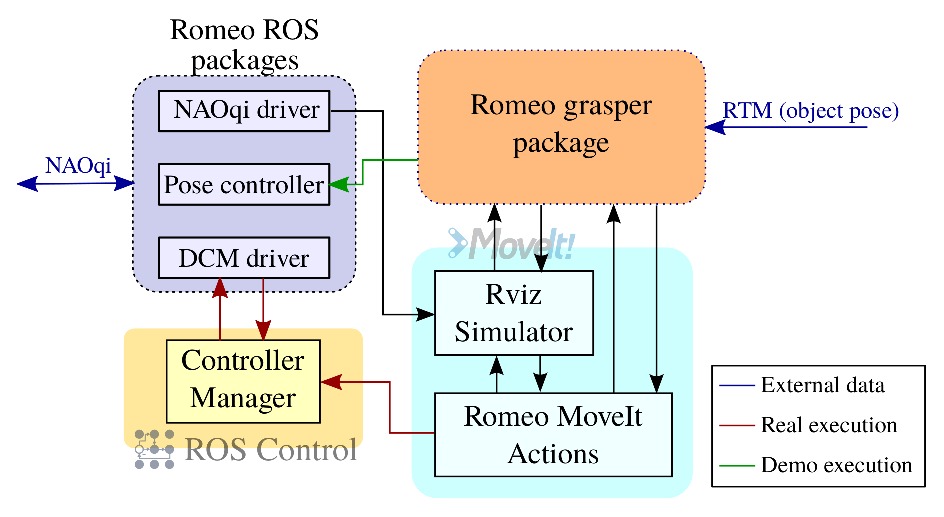
\includegraphics[width=0.8\textwidth]{images/move_control_overview.eps}
\caption{Flow of data from object pose to commands to NAOqi\label{fig:communication_all_packages}}
\end{figure}

%TODO
%Revisar si la taula esta ben organitzada
\begin{table}[!h]
\begin{center}
\begin{tabulary}{0.95\textwidth}{|l|l|l|p{18.5em}|}
\hline
\textbf{Sender} & \textbf{Receiver} & \textbf{Data} & \textbf{Description}\\ \hline
V4R & \specialcell{l}{Romeo\\grasper} & \specialcell{l}{Object\\pose} & Information of the object position and the confidence of the tracker \\ \hline 
\specialcell{l}{Romeo\\grasper} & \specialcell{l}{MoveIt\\Actions} & Commands & Commands to plan, execute, pick or set parameters to the \texttt{move\_group}. \\ \hline
\specialcell{l}{MoveIt\\Actions} & \specialcell{l}{Romeo\\grasper} & Results & Returns the results of the commands sent, like if it is succeeded, the trajectory planned or the final planned pose. \\ \hline
\specialcell{l}{Rviz\\Simulator} & \specialcell{l}{Romeo\\grasper} & Link poses & Position of some elements like the wrist or the camera are sent to calculate the camera pose or the object pose.  \\ \hline
\specialcell{l}{Romeo\\grasper} & \specialcell{l}{Rviz\\Simulator} & Link poses & Position of the camera and of the object. \\ \hline
\specialcell{l}{NAOqi\\driver} & \specialcell{l}{Rviz\\Simulator} & Joint state & Simulator needs the joint state to have the simulated robot as the real one. \\ \hline
\specialcell{l}{MoveIt\\Actions} & \specialcell{l}{Rviz\\Simulator} & Commands & Commands to calculate a plan and simulate to check collisions.  \\ \hline
\multicolumn{4}{|r|}{\small\sl continued on next page}\\
\hline
\end{tabulary}
\end{center}
\end{table}

\newpage

\begin{table}[!h]
\begin{center}
\begin{tabulary}{0.95\textwidth}{|l|l|l|p{18.5em}|}
\hline
\multicolumn{4}{|l|}{\small\sl continued from previous page}\\ \hline
\textbf{Sender} & \textbf{Receiver} & \textbf{Data} & \textbf{Description}\\ \hline
\specialcell{l}{Rviz\\Simulator} & \specialcell{l}{MoveIt\\Actions} & Results & Returns if it is succeeded or the trajectory planned.  \\ \hline
\specialcell{l}{MoveIt\\Actions} & \specialcell{l}{Controller\\Manager} & \specialcell{l}{Execution\\Plan} & Sends the plan which should be execute on the real robot. \\ \hline
\specialcell{l}{Controller\\Manager} & DCM driver & Commands & Commands with the right timing to have a real-time control with the Romeo robot. \\ \hline
DCM driver & \specialcell{l}{Controller\\Manager} & Joint state & Controller Manager should be update constantly with the Romeo state in order to be able of having a real-time control. \\ \hline
\specialcell{l}{Romeo\\grasper} & \specialcell{l}{Pose\\controller} & Trajectory & In case of simulated robot, it sends the trajectory to be executed. \\ \hline
Romeo ROS & NAOqi & Commands & Commands to move the robot and to get specific information. \\ \hline
NAOqi & Romeo ROS & Data & All kind of data: joint state, camera images, variable names, etc. \\ \hline
\end{tabulary}
\caption{Information sent and received from and to the packages. \label{tab:info_flow_packages}}
\end{center}
\end{table}

\chapter{Experiments}
\label{cha:experiments}
% Explicar els experiments que s'han anat fent durant tot el proces (talvegada nombrats anteriorment en la implementació) juntament amb les mesures que es prenen per fer les coses.
% S'ha de mirar de que tot experiment tengui una certa mesura per veure si ha anat més bé o més malament.
% Un test que es pot fer es per comparar els dos IK, fent proves anant a les mateixes posicions veure quin error tenen cadascun. Si IKFast no arriba a poder ser implementat a nes experiments es pot posar ses diferents coses que s'han fet per mirar d'aconseguir-ho. Primer dir amb es urdf inicial que hi havia s'han fet proves de tots es tipus tant des de torso, base_link com des de L/RShoulder. Aquesta última fins a gripper ha sigut l'única que ha funcionat pero que no té molt de sentit perque el L/RShoulderPitch no esta inclos a dins i per tant es perd aquest grau de llibertat que dona un desplaçament molt important per arribar a diferents punts.

\section{Movement in simulation}
%Experiment 1:
% Moviment a llista de posicions determinades amb reachAction i provar mateixa llista amb graspPlan. Per això s'haura d'adaptar la forma com es calcula la diferencia amb el graspPlan. A més si es pogues tenir una referencia del temps que tarda millor (ja que el graspPlan tarda bastant). Amb aquest experiment es veu l'error que pot arribar a tenir el IK solver.
% També pot ser que l'error es trobi en el forward kinematics que no doni exactament la posició que toca. Per això s'hauria de comprovar que el TF dona la mateixa posicio que el forward quan s'ha executat la trajectoria i veient que les joints estan en la mateixa posicio que la trajectoria. S'ha vist que l'error entre el FK i l'execució en simulació es nomes de decimes de milimetre, per tant despreciable.
%Una posible solucio per no tenir problemes amb el graspPlan podria ser posar momentaneament que el romeo_grasp_data.yaml que no hi ha diferencia de posicio entre eef i grasp. D'aquesta forma la solució  seria exacte, l'únic problema es que no seria realista ja que Wrist aniria sobre l'objecte.
\begin{itemize}
\item Given a list of position where it is supposed to be the object. Test theses with \texttt{reachAction} and \texttt{graspPlan}.
\item Try with different planning times.
\item The problem doesn't come from the forward kinematic that calculate the difference between pose target and pose plan because it has been test to see if the calculated and the real one, with the values of the joint as the trajectory, are in the same position and yes, the difference is about of the order of $10^-4 m$.
\item To do this experiment is used the Python program named \texttt{experiment1.py}.
%TODO explaination of the program??
\end{itemize}

\section{Implementation IKFast on Romeo}
\label{sec:exp_ikfast}

Currently, the inverse kinematic solver used is from the KDL library, explained in Section \ref{sec:inverse_kinematic}. However, it gives bad results as shown above. Therefore, a solution for this problem could be implement the IKFast solver, also explained in Section \ref{sec:inverse_kinematic}, which is faster and more precise. 

In order to implement the IKFast on the Romeo robot, firstly is needed to generate the C++ code which solve the inverse kinematics. However, This OpenRAVE software has several dependencies to generate the C++ code, explained with the installation in Section \ref{app:ikfast}. Secondly, once the code is already generated, it should be create a package which provides the kinematic solver, based on the previous C++ code. Although, it is needed to have the \texttt{moveit\_ikfast} ROS package to create the kinematic solver package. 

Referring to the code, it is created from a Collada model file which is not found in the \texttt{romeo\_description} package. Then, this can be created, using the command below, from an URDF model of Romeo which is contained in the previous package.

\begin{lstlisting}[language=ROS]
rosrun collada_urdf urdf_to_collada romeo.urdf romeo_raw.dae
\end{lstlisting}

After that, as recommended by the author of IKFast  \cite{Diankov2010}, it is good to round at the fifth decimal the values of the Collada model to make easier to find aligned axes. The rounding program is found in the \texttt{moveit\_ikfast} package, more information in \cite{MoveIt2013}, and is run with the following command:

\begin{lstlisting}[language=ROS]
rosrun moveit_ikfast round_collada_numbers.py <myrobot_name>.dae <myrobot_name>.rounded.dae 5
\end{lstlisting}

Once the Collada model is ready, it is time to generate the IKFast solver code. As said in Section \ref{sec:romeo_hardware}, the Romeo arms have 7 DoF, so the inverse kinematic type should be \texttt{transform6d} with one redundancy to be able to go to a specific position and orientation. Moreover, has to be defined which is the base link and the end effector of the group. So between these are contained the joints of the arm, Table \ref{tab:tree_group_links_joint} can help to know parent and child link for every joint. The index of the arm links of Romeo are shown in Table \ref{tab:link_index_ikfast}. 

\begin{table}[!h]
\begin{center}
\begin{tabular}{|c|c|}
\hline
\multicolumn{2}{|c|}{\textbf{Body}} \\ \hline
\textbf{Link} & \textbf{index} \\ \hline
base\_link & 0 \\
torso & 1 \\
\end{tabular}
\\
\begin{tabular}{|l|c|c|c|r|}
\hline
\multicolumn{2}{|c|}{\textbf{Left arm}} & & \multicolumn{2}{|c|}{\textbf{Rigth arm}} \\ \cline{1-2}\cline{4-5}
\textbf{Link} & \textbf{index} & & \textbf{index} & \textbf{Link} \\ \cline{1-2}\cline{4-5}
LShoulder & 2 & & 43 & RShoulder \\
LShoulderYaw\_link & 3 & & 44 & RShoulderYaw\_link \\
LForeArm & 4 & & 45 & RForeArm \\
LElbow & 5 & & 46 & RElbow \\                            
LWristRoll\_link & 6 & & 47 & RWristRoll\_link \\                   
LWristYaw\_link & 7 & & 48 & RWristYaw\_link \\ \cline{1-2}\cline{4-5}
l\_wrist & 8 & & 49 & r\_wrist \\
l\_gripper & 18 & & 59 & r\_gripper \\ \hline
\end{tabular}
\caption{Index of every link of the robot base and arms.\label{tab:link_index_ikfast}}
\end{center}
\end{table}

Therefore, the generation process is executed with the command below. Finally, it should be stated that if for the configuration are contained 7 joints, it should be add the \texttt{freeindex} parameter defining which is a free joint.\footnote{The free joints are specified before the IK is run, these values are known at runtime, but not known at IK generation time \citep{Diankov2010}.} The index for the joints is shown in Table \ref{tab:joint_index_ikfast}.

\begin{lstlisting}
python `openrave-config --python-dir`/openravepy/_openravepy_/ikfast.py --robot=<myrobot_name>.rounded.dae --iktype=transform6d --baselink=<base_index> --eelink=<end_effector_index> --savefile=<ikfast_output_path>
\end{lstlisting}

\begin{table}[!h]
\begin{center}
\begin{tabular}{|l|c|c|c|r|}
\hline
\multicolumn{2}{|c|}{\textbf{Left arm}} & & \multicolumn{2}{|c|}{\textbf{Rigth arm}} \\ \cline{1-2}\cline{4-5}
\textbf{Joint} & \textbf{index} & & \textbf{index} & \textbf{Joint} \\ \cline{1-2}\cline{4-5}
LShoulderPitch & 0 & & 16 & RShoulderPitch \\
LShoulderYaw & 1 & & 17 & RShoulderYaw \\
LElbowRoll & 2 & & 18 & RElbowRoll \\
LElbowYaw & 3 & & 19 & RElbowYaw \\                            
LWristRoll & 4 & & 20 & RWristRoll \\                   
LWristYaw & 5 & & 21 & RWristYaw \\ \cline{1-2}\cline{4-5}
LWristPitch & 6 & & 22 & RWristPitch \\
LHand & 7 & & 23 & RHand \\ \hline
\end{tabular}
\caption{Index of every joint of the robot arms.\label{tab:joint_index_ikfast}}
\end{center}
\end{table}

After that, it is time to generate the IK solver code. As explained in Section \ref{sec:romeo_hardware}, the usually way of working is to split the arm in two group. So the right way is to take the first 6 joint of the arm in the main group which is the one controlling the position and orientation. Therefore, the logical configuration is with \texttt{--eelink} equal to 7 or 48 depending on the left or right arm and \texttt{--baselink} equal to 0 or 1.\footnote{It doesn't matter if is used \texttt{base\_link} or \texttt{torso} link because they are fixed, so there is only a fixed transformation between them.}

Unfortunately any of this configuration can generate a C++ code with the Romeo model. The problem is that, after one or two hours of execution of the command above, the program, and sometime also the computer, is frozen. Then, it has to be tested others configuration which are less logical but also useful. Therefore, these are taking the 7 joints but adding the \texttt{freeindex} parameter. The most logical free joint is the \texttt{WristRoll} because is the one closest to the end effector, doing the same movement than \texttt{ElbowRoll} and it is the slowest joint of the arm. Finally, neither this configuration nor any other joint as the free joint can generate the IK solver code.

Currently, there is a commit in the Natalia Lyubova repository\footnote{\url{https://github.com/nlyubova/romeo_robot/commit/05bf217b73c389c461414412fd43d84ecb0c4115}} where the URDF model has been changed to use a new convention of the joints. But, it also has the same result. 

It should be stated that to be sure the installation it was well done, it has been tried to generate the IKFast for another robot and it worked. Moreover, there is a discussion in the official repository of Romeo package where all this IKFast issue is discussed \cite{romeoRobotIssue}. 

\section{Get pre-known camera position}
%Experiment 3:
% En vista que no es pot fiar de la posicio extreta a partir de la propia camera s'ha de mirar de treure la posicio de la camera de forma empirica. Mirar a veure com es pot ser es màxim d'exacte possible. Una manera podria ser com que lo més dificil de posicionar es respecte X i Z ja que esta inclinat, es podria mirar de fer que el l_wrist estigui alineat amb la camera en l'eix Y i per tant X i Z es mantenen iguals.
\begin{itemize}
\item Get the position of the camera respect to the robot empirically
\item The difficulty is with X and Z axes (robot reference) because the robot is tilted. So if the Wrist is align with the camera on the Y axe, then knowing the position of Wrist (given by the simulator) we have the X and Z of the camera.
\end{itemize}

\section{Visual camera positioning}
%Experiment 4:
% Experiments sobre el posicionament de la camera. Pendre mesures aproximades d'on es troba la camera i orientació respecte el robot i provar els diferents algorismes a veure si funcionen. (ja es tenen es arxius amb ses dades, es mirar de treure algo en clar). Talvegada es pot jugar amb es seeds que es donen en plan provar 3 seeds un molt generic un altra mes proper i finalment es que es sa mesura que mus hauria de donar.
% Talvegada s'hauria de repetir el testejat, ja que es cert que si esta sense Stiffness dona un cert error entre la realitat i el model
% A més dir que les mesures que pren la camera d'on es troba cadascuna de les parts ha estat contrastada empiricament per veure que la mesura era correcte. I si era correcte amb un error de +-2cm.
%Antes de fer aço millor mirar de tenir el valor exacte de la inclinació.
\begin{itemize}
\item Use the previous measures
\item Compare this with the results of applying the proposed algorithm 
\item Test with different seed, from a general seed to a specific one very close to the real solution.
\item Possibles errors:
\begin{itemize}
\item When is measured where is the camera in robot reference (may be an error of $\pm$ 1.5 cm)
\item Error in positioning the parts of the robot with the reference object (may be an error of $\pm$ 2 cm)
\end{itemize}
\end{itemize}

\section{Error produces by the camera positioning}
%Experiment 5:
% Per comprovar l'error que es té de la posició i orientació de la camera es pot mirar d'identificar un objecte en una posició determinada, veure el valor que dona de l'objecte i finalment dur el wrist del robot a la posició de tal manera que es pugui veure en quant s'ha equivocat la càmera.
\begin{itemize}
\item Identify an object in a specific position, see the result in robot reference. Then compare this result with the value given by the simulator putting there the Wrist of the robot.
\end{itemize}

\chapter{Discussion}
\label{cha:discussion}
% Aqui s'expliquen quines interpretacions es fan des resultats obtinguts.
% Com que es vol que es millori el conjunt per a que sigui més lliure pues s'han fet millores en els packages corresponents (NOSE ALGO).

\chapter{Future works}
\label{cha:future_works}
% Explicar coses que s'han fet que no han acabat de funcionar o que  Posar en una posició inicial seguint un path, d'aquesta manera s'assegura que no fer-hi la taula ja que a la simulació sembla que obvia el fet que hi hagi la taula.
% Com també per on es podria tirar per millorar tot es conjunt
\section{Implementation new inverse kinematics}

As said before, the error produced by the inverse kinematic solver KDL to go to the position of the object is one of the most important. Therefore, the implementation of a new IK solver should be a great improvement for the work. Moreover, currently the picking action is not working well due to the IK solver doesn't find a good picking plan, so with this new solver it is supposed that this should be solved.

The first recommendation would be to implement the IKFast from OpenRAVE, because it is a close form solver and so it very fast and precise. As seen in Section \ref{sec:exp_ikfast}, currently is not working, but may be can solve it editing the URDF model trying to make it easier or changing the initial pose. Also is recommended to read this issue \cite{romeoRobotIssue}, where there is a lot about it discussed.

In case that the previous solver could not be used, there is an other option used in \cite{claudio:hal-01159882} named Metapod from LAAS, which is also a numerical solver. Therefore, probably it has almost the same problems as KDL, but at least has been already tested with Romeo.  

\section{Improve use of V4R}

The V4R software is a very powerful tool to recognise objects and tracking them. However, it has to be complemented with the convenient camera to get the best performance. Currently, the Kinect camera, which sends the images to ROS through OpenNi framework, gives some problems. On one hand, after some seconds or minutes the RGB camera starts to send partial or full black images, example of it in Figure \ref{fig:kinect_black_problem}. Therefore, the V4R software cannot be used properly. On the other hand, the OpenNi nodes after a while usually fail due to memory or pointers errors and then they are automatically shut down.

\begin{figure}[h]
\begin{center}
\begin{subfigure}[r]{0.65\textwidth}
		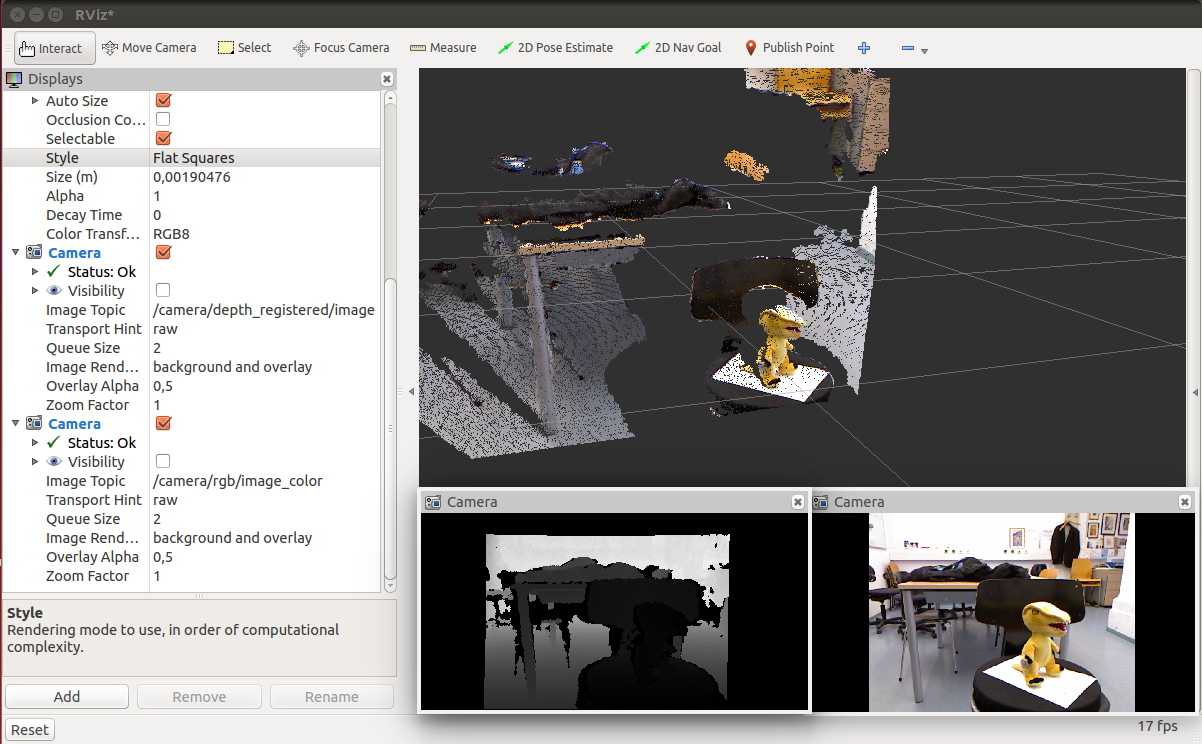
\includegraphics[width=\textwidth]{images/kinect_problem_color}
        \caption{Normal performance}
\end{subfigure}
\\
\begin{subfigure}[r]{0.65\textwidth}
		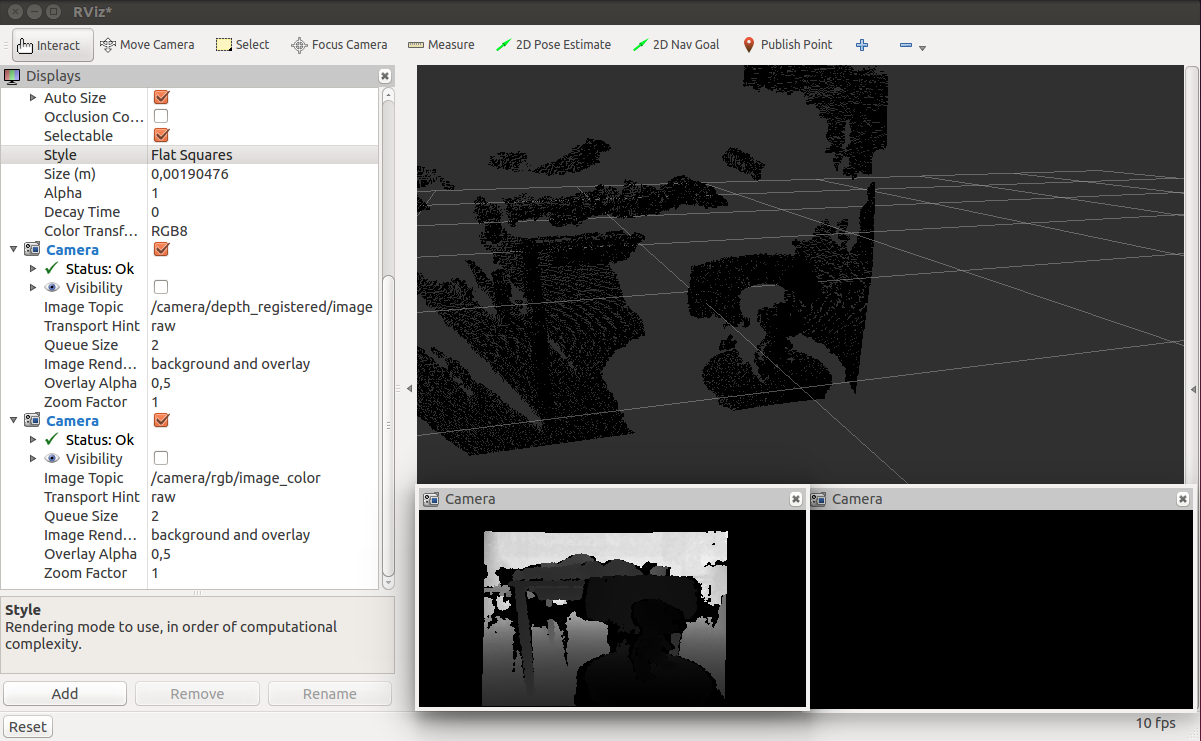
\includegraphics[width=\textwidth]{images/kinect_problem_black}
        \caption{While is not working}
\end{subfigure}
\caption{Kinect problem, RGB camera sending black images.\label{fig:kinect_black_problem}}
\end{center}
\end{figure}

Moreover, V4R process the images with a kind of SIFT on the RGB image, so having a good quality of the RGB camera it could lead to a better performance. Unfortunately, the Kinect used is the worst in terms of RGB camera in comparison with the Xtion and the RealSense, as shown in Table \ref{tab:camera_comparison}. Therefore, to improve the performance of the recognition would be great to use RealSense or Xtion. On one hand, currently, the use of RealSense is possible,\footnote{The \texttt{use\_realsense} argument enables to launch the \texttt{romeo\_grasper} using the RealSense camera.} but the object must be modeled with another camera because RealSense is not supported by RTM-Toolbox and that decrease dramatically the confidence of the tracking. Therefore, this option would be great if the RTM-Toolbox is improved and gives support to RealSense. On the other hand, for the Xtion there are two possibilities. First, with an external one as it has been done with Kinect in this work. Second, using the one on the Romeo cap. For this last one, only could work with objects on a specific and small range because of the camera range. However, it would remove some error produced by the camera positioning because the position of this camera is established in the model. Moreover, in order to solve the problem with dark images may be a possibility is to try to execute ROS with OpenNi inside the robot.  

\begin{table}[h]
\begin{center}
\begin{tabular}{|l|c|c|c|}
\hline
\textbf{Camera} & \textbf{RGB resolution} & \textbf{Depth resolution} & \textbf{Range} \\ \hline
Microsoft Kinect v1 \cite{Smeenk}& 640x480 & 320x240 & 0.5-4.5 m \\
ASUS Xtion PRO Live \cite{ASUSWeb}& 1280x1024 & 640x480 & 0.8-3.5 m \\
RealSense SR300 \cite{IntelWeb}& 1920x1080 & 640x480 & 0.2-1.5 m \\ \hline
\end{tabular}
\caption{Comparison of the RGB-D cameras: Kinect, Xtion and RealSense.\label{tab:camera_comparison}}
\end{center}
\end{table}

\section{Object identification}
\label{sec:object_ident}

Although, it is not explained before, V4R has another feature which allows to recognise several objects at once. These objects should be in a specific database. A detailed description of this feature can be found in the tutorial of V4R ROS wrappers repository \cite{gitV4RWrappers}. There are several factors of the object recognition that can improve the performance of the \texttt{romeo\_grasper} package:

\begin{itemize}
\item Provides the centroid of the cluster, which could be used to give to the package where it have to make the grasp.
\item Provides a bounding box of the object, which is how the object is represent in the simulation by now. So this would make to don't need to use a custom bounding box made by the user.
\item Provides a point cloud of the model transformed into camera coordinates. This information could be used for the AGILE grasp to grasp the desired object in a better way.
\item Identifying several objects at one could be used to implement a better way to use the visual positioning of the camera. Using a different identifier for every element could be possible to know the position of every link at once. Therefore, it makes the process more robust to find the camera position and orientation. 
\end{itemize}

The only problem of this way of get the position of the object is that it is not optimal for a real-time tracking. This feature works as a service, so in order to work with it, the service should be called periodically to know always where are the object.

\section{Fix the Romeo model}

Currently, the grippers in the Romeo model are posed in a wrong position, see Figure \ref{fig:gripper_bad_position}. However, at the moment, this is not used because the grasp position is specified by \texttt{romeo\_grasp\_data.yaml} of the \texttt{moveit\_simple\_grasps} package. Then, the grasp position is set adding an offset from the WristYaw\_link position. Therefore, should be great to make the model more standard and have the gripper in the right place and set the grasp from the gripper itself. 

\begin{figure}[h]
\centering
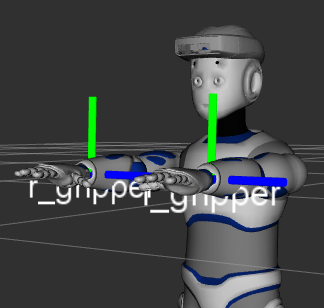
\includegraphics[width=0.5\textwidth]{images/gripper_bad_position.png}
\caption{Current position of grippers in Romeo model.\label{fig:gripper_bad_position}}
\end{figure}

\section{Implementation of AGILE grasp}

Once the first approach of grasping works perfectly, it is time to implement a more advanced grasping process. As explained in Section \ref{sec:agile grasp}, the AGILE grasp use machine learning to detect a antipodal grasp pose on novel objects, using as input a point cloud and the geometric parameters of the robot hand. However, the implementation could be made in two different ways. First, it could use the general point cloud of the camera which it will have some occluded parts of the object. Second, if the recognition object, explained in Section \ref{sec:object_ident}, is implemented then use the point cloud of the model transformed into camera coordinates which it won't have occluded parts because it is a combination of the modeled object and the real object. 

\section{Dependencies of packages}

A package is more flexible and can be reused in other fields as independent is of other packages. On one hand, it would be great to make this package as general as possible, in order to be able to be used for other robots. That could be made if the \texttt{romeo\_moveit\_actions} have the same functions of the moveit actions of others robots, then it is supposed that it should not be very difficult with the right definitions for the building part. On the other hand, making the code be independent of the recognition software could lead to used this grasping package in a wider range of fields.


\chapter{Conclusion}
\label{cha:conclusions}
% Explicar a les conclusions que s'arriben finalment i els posible futurs treballs que se'n poden derivar.

\bibliography{./library/library}
\addcontentsline{toc}{chapter}{References}
\label{cha:references}

\appendix
\clearpage % o \cleardoublepage
\addappheadtotoc
\appendixpage

\renewcommand{\thefigure}{\thechapter.\arabic{figure}}
\renewcommand{\thetable}{\thechapter.\arabic{table}}
\renewcommand{\theequation}{\thechapter.\arabic{equation}}
\renewcommand{\thefootnote}{\arabic{footnote}}

%\newcommand{\appendixpagenumbering}{
%  \break
%  \pagenumbering{arabic}
%  \renewcommand{\thepage}{\thechapter-\arabic{page}}
%}
%
%\appendixpagenumbering
\chapter{Software requirements and installation}
\section{Software requirements}

In this study there are some software that must be installed to be able to do it. Here it is explained briefly which are these software and their installation. Firstly, a table with the software required with his version \ref{tab:soft_req}.

\begin{savenotes}
\begin{table}[h]
\begin{center}
\begin{tabular}{l|c|}
Software & Version\\ \hline
Ubuntu & 14.04\\
ROS & Indigo\\
Choregraphe & 2.1.4.5 (1.14.5)\footnote{\label{fn:nao_version}NAO robot use version 1.14.5 and Romeo use 2.1.4.5. So if you want to test first in Nao like in this master thesis you need both versions.}\\
C++ NAOqi SDK & 2.1.4.5 (1.14.5)\cref{fn:nao_version}\\
QiBuild & from installation\footnote{Recommended installing using \texttt{pip} as is said in qiBuild documentation \cite{AldebaranQiBuild}}\\
QtCreator & recent\footnote{As is said in NAO documentation \cite{AldebaranC++SDK}}\\
\end{tabular}
\caption{Software required with his version\label{tab:soft_req}}
\end{center}
\end{table}
\end{savenotes}

\section{Camera drivers installation}
\label{app:camera_instal}

In order to install the Kinect camera with openNi has been used the following url \cite{Li}. For the RealSense camera has been used this repository \cite{gitRealSense} following the installation instructions. Unfortunately, the Asus Xtion camera has not been possible to use so here there is no description about the installation.

\section{OpenRAVE installation}
\label{app:ikfast}
 

\end{document}